%% Copernicus Publications Manuscript Preparation Template for LaTeX Submissions
%% ---------------------------------
%% This template should be used for copernicus.cls
%% The class file and some style files are bundled in the Copernicus Latex Package which can be downloaded from the different journal webpages.
%% For further assistance please contact the Copernicus Publications at: publications@copernicus.org
%% http://publications.copernicus.org


%% Please use the following documentclass and Journal Abbreviations for Discussion Papers and Final Revised Papers.


%% 2-Column Papers and Discussion Papers
\documentclass[gmd, manuscript]{copernicus}



%% Journal Abbreviations (Please use the same for Discussion Papers and Final Revised Papers)

% Atmospheric Chemistry and Physics (acp)
% Advances in Geosciences (adgeo)
% Advances in Statistical Climatology, Meteorology and Oceanography (ascmo)
% Annales Geophysicae (angeo)
% ASTRA Proceedings (ap)
% Atmospheric Measurement Techniques (amt)
% Advances in Radio Science (ars)
% Advances in Science and Research (asr)
% Biogeosciences (bg)
% Climate of the Past (cp)
% Drinking Water Engineering and Science (dwes)
% Earth System Dynamics (esd)
% Earth Surface Dynamics (esurf)
% Earth System Science Data (essd)
% Fossil Record (fr)
% Geographica Helvetica (gh)
% Geoscientific Instrumentation, Methods and Data Systems (gi)
% Geoscientific Model Development (gmd)
% Geothermal Energy Science (gtes)
% Hydrology and Earth System Sciences (hess)
% History of Geo- and Space Sciences (hgss)
% Journal of Sensors and Sensor Systems (jsss)
% Mechanical Sciences (ms)
% Natural Hazards and Earth System Sciences (nhess)
% Nonlinear Processes in Geophysics (npg)
% Ocean Science (os)
% Primate Biology (pb)
% Scientific Drilling (sd)
% SOIL (soil)
% Solid Earth (se)
% The Cryosphere (tc)
% Web Ecology (we)



%% \usepackage commands included in the copernicus.cls:
%\usepackage[german, english]{babel}
%\usepackage{tabularx}
%\usepackage{cancel}
%\usepackage{multirow}
%\usepackage{supertabular}
%\usepackage{algorithmic}
%\usepackage{algorithm}
%\usepackage{float}
%\usepackage{subfig}
%\usepackage{rotating}

\usepackage{amsmath}
\usepackage{lineno}	% Dominik linenumbers
\usepackage{rotating}	% Dominik rotate table
\usepackage{amssymb}

\usepackage{marginnote} %Dominik for commments during drafting
\setlength{\marginparwidth}{35mm}

\usepackage{empheq}
\definecolor{myblue}{rgb}{.8, .8, 1}
\newlength\mytemplen
\newsavebox\mytempbox

\makeatletter
\newcommand\mybluebox{%
    \@ifnextchar[%]
       {\@mybluebox}%
       {\@mybluebox[0pt]}}

\def\@mybluebox[#1]{%
    \@ifnextchar[%]
       {\@@mybluebox[#1]}%
       {\@@mybluebox[#1][0pt]}}

\def\@@mybluebox[#1][#2]#3{
    \sbox\mytempbox{#3}%
    \mytemplen\ht\mytempbox
    \advance\mytemplen #1\relax
    \ht\mytempbox\mytemplen
    \mytemplen\dp\mytempbox
    \advance\mytemplen #2\relax
    \dp\mytempbox\mytemplen
    \colorbox{myblue}{\hspace{1em}\usebox{\mytempbox}\hspace{1em}}}

\makeatother
\begin{document}

%\linenumbers

\title{OMEN-SED 1.0: A new, numerically efficient sediment module for the coupling to Earth System Models}


% \Author[affil]{given_name}{surname}
\Author[1]{Dominik}{H\"ulse}
\Author[1, 2]{Sandra}{Arndt}
\Author[3]{Stuart}{Daines}
\Author[2]{Pierre}{Regnier}
\Author[1, 4]{Andy}{Ridgwell}

\affil[1]{School of Geographical Sciences, University of Bristol, Clifton, Bristol BS8 1SS, UK}
\affil[2]{Department of Earth and Environmental Sciences, Universit\'e Libre de Bruxelles, Brussels, Belgium}
\affil[3]{Earth System Science, University of Exeter, North Park Road, Exeter EX4 4QE, UK}
\affil[4]{Department of Earth Sciences, University of California, Riverside, CA 92521, USA}

%% The [] brackets identify the author with the corresponding affiliation. 1, 2, 3, etc. should be inserted.



\runningtitle{OMEN-SED 1.0 - a sediment model for Earth system models}

\runningauthor{H\"ulse et al.}

\correspondence{Dominik H\"ulse (Dominik.Huelse@bristol.ac.uk)}



\received{}
\pubdiscuss{} %% only important for two-stage journals
\revised{}
\accepted{}
\published{}

%% These dates will be inserted by Copernicus Publications during the typesetting process.


\firstpage{1}

\maketitle



\begin{abstract}
Here we describe the first version of a new, analytical early diagenetic model resolving organic matter cycling and associated biogeochemical dynamics in marine sediments called OMEN-SED (Organic Matter ENabled SEDiment model). 
Most biogeochemical cycles and reactions in the surface sediments can be related either directly or indirectly to the degradation of organic matter. 
Despite its fundamental importance, an appropriate Earth system model of the coupled atmosphere-ocean-sediment system which is able to model all 
relevant processes and feedbacks over geological time-scales currently does not exist. The major problem is the high computational cost of simulating 
the essential redox reactions in marine sediments which are important to calculate burial of organic matter and benthic recycling fluxes of chemical compounds. 
In most Earth system models sediment-water dynamics are  either neglected or treated in a very simplistic way. To provide a more realistic description of organic matter 
degradation and nutrient cycles in marine sediments we have developed OMEN-SED, a new, one-dimensional, numerically efficient reactive transport model. 
OMEN-SED is the first analytical model to explicitly describe organic matter cycling as well as associated dynamics of the most important terminal electron acceptors (i.e. \chem{O_2} , \chem{NO_3}, \chem{SO_4}), 
related reduced substances (\chem{NH_4}, \chem{H_2S}), the full suite of secondary-redox reactions, macronutrients (\chem{PO_4}) and associated pore water quantities (\chem{ALK}, \chem{DIC}). 
To represent a redox-dependent sedimentary P cycle we consider the formation and burial of Fe-bound P and authigenic Ca-P minerals. 
Thus, OMEN-SED captures most of the features of a complex, numerical diagenetic model, however, its computational efficiency allows the coupling to global Earth System models 
and therefore the investigation of coupled global biogeochemical dynamics over different timescales. This paper provides a detailed description of the new sediment 
model, \textcolor{red}{tested with observations, SA and global observations} and describes it's coupling to the Earth System model cGENIE.
\end{abstract}

%\newpage

\tableofcontents

\newpage


\introduction  %% \introduction[modified heading if necessary]
\textbf{Dominik: Introduction needs polishing, this is my first draft}\\

%>>>
\marginnote{\textbf{DH}: Will delete the sub-headings!}[-1cm]%<<<
\textbf{Role of marine sediments for climate and global biogeochemical cycles:}\\
Marine surface sediments are key components in the Earth system. They host the largest carbon reservoir within the surficial Earth system, provide the only long term sink for atmospheric \chem{CO_2}, 
recycle nutrients and represent the most important geochemical archive used for deciphering past changes in biogeochemical cycles and climate  \citep[e.g.][]{berner:91, archer_effect_1994, ridgwell_role_2005, arndt_quantifying_2013}. 
Physical and chemical processes in sediments (i.e. diagenetic processes) depend on the water column and vice versa: Diagenesis is controlled by the external supply of solid material 
(e.g. organic matter, calcium carbonate, opal) from the water column and is affected by overlying bottom water concentrations of solutes. 
At the same time, sediments impact the water column directly either by short- and long-term storage of deposited material or diagenetic processing of deposited material and 
diffusion of some of the resulting products (e.g. nutrients, DIC) to the overlying bottom waters. 
This so-called benthic-pelagic coupling is essential for understanding global biogeochemical cycles and climate \citep[e.g.][]{archer_effect_1994, archer_what_2000, soetaert_coupling_2000, mackenzie_sediments_2005}. 

Biological primary production of organic matter (OM, \chem{CH_2O} in equation \ref{eq:photosynthesis}) and the reverse process of degradation can be written in a greatly simplified reaction as:
\begin{reaction}
\chem{CO_2}+\chem{H_2O} \rightleftharpoons \chem{CH_2O} + \chem{O_2}.\label{eq:photosynthesis}
\end{reaction}
On geological timescales production of OM is generally greater than degradation which results in some organic matter being buried in marine sediments and oxygen accumulating in the atmosphere. 
Thus burial of OM leads to net oxygen input to, and \chem{CO_2} removal from the atmosphere \citep{berner_phanerozoic_2004}. 
On shorter timescales, the upper few meters of the sediments where early diagenesis occurs are specifically important as this zone controls whether a substance is recycled 
to the water column or buried for a longer period of time in the deeper sediments \citep{hensen_benthic_2006}. 
Most biogeochemical cycles and reactions in this part of marine sediments can be related either directly or indirectly to the degradation of organic matter \citep[][]{arndt_quantifying_2013}. 
Oxygen and nitrate for instance, the most powerful electron acceptors, are consumed in the course of the degradation of organic matter, resulting in the release of ammonium and phosphorus to the pore water. 
As such, degradation of OM in the sediments can profoundly affect the oxygen and nutrient inventory of the ocean and thus primary productivity \citep{van_cappellen_benthic_1994, lenton_redfield_2000}. 
Furthermore, organic matter degradation releases metabolic \chem{CO_2} to the pore water, causing it to have a lower pH and provoking the dissolution of calcium carbonate \chem{CaCO_3} \citep{emerson_carbon_1981}.

% DH: more facts on sediments
%Furthermore, the sedimenst form an important sink for organic phosphorus and nitrogen. 
%Furthermore, burial of OM represents an important connection between carbon stored in more climate-relevant reservoirs like oceans, atmosphere, 
%and surficial sediments and carbon that is sequestered for much longer, geological timescales in sedimentary rock or coal \citep{mackenzie_sediments_2005, burdige_preservation_2007}. 

% \textcolor{red}{TODO include info on shelf-nutrient hypothesis:} (From Palastanga et al. 2013) 
% During  glacial  periods,  P  burial  on  shelves was likely reduced because of sea level fall, whereas the 
% erosive transfer of particulate material containing reactive P and degradable carbon from shelves to the open ocean was likely
% enhanced (Ruttenberg,1993). As a consequence, the inventory of P in the open ocean, primary productivity and CO2 
% drawdown may have increased, whereas ocean oxygen may have declined. This potential impact on productivity and CO2 
% was first brought forward by Broecker (1982) in the so-called shelf-nutrient hypothesis.

Nutrient recycling from marine sediments has been suggested to play a key role for climate and ocean biogeochemistry for different events during Earth history. 
For example, feedbacks between phosphorus storage and erosion from shelf sediments and marine productivity have been hypothesised to play an important role for glacial/interglacial atmospheric \chem{CO_2} changes \citep{broecker_ocean_1982, ruttenberg_reassessment_1993}. 
Furthermore, nutrient recycling from anoxic sediments has been invoked to explain the occurance of more extreme events in Earth history, for instance Oceanic Anoxic Events % by modelling and data studies 
\citep[OAEs, e.g.][]{mort_phosphorus_2007, tsandev_modeling_2009}. OAEs represent severe disturbances of the global carbon, oxygen and nutrient cycles of the ocean and are usually characterized 
by widespread bottom water anoxia and photic zone euxinia \citep{jenkyns_geochemistry_2010}. 
One way to explain the genesis and persistence of OAEs is increased oxygen demand due to enhanced primary productivity. Increased nutrient inputs to fuel primary productivity may have come from marine sediments as the 
burial efficiency of phosphorus declines when bottom waters become anoxic \citep{ingall_evidence_1994, van_cappellen_benthic_1994}. 
The recovery from OAE like conditions is thought to involve the permanent removal of excess \chem{CO_2} from the atmosphere and ocean by burying carbon in the form of organic matter in marine sediments 
\citep[e.g.][]{arthur_geochemical_1988, jarvis_black_2011}, which is consistent with the geological record of widespread black shale formation \citep{stein_accumulation_1986}. 
However, the overall amount, exact timing and the rate of organic matter burial remain a topic of an ongoing debate. 
Therefore, globally quantifying the burial and degradation of organic matter in marine sediments and related biogeochemical dynamics is important for understanding 
climate and the cycling of many chemical elements on various timescales. 

% % Difference for oxic vs. anoxic sediments and impacts on atmospheric \chem{CO_2}. 
% % 
% % Give examples when and why important (also in Paleo-context).\\
% % 
% % - general dynamics: first e.g. \chem{CaCO_3} then nutrients and the OM! \\
% % - then more focus on paleo!\\
% % - glacial/interglacial atmospheric p\chem{CO_2} cycles\\ 
% % - maybe important for OMZ (see Kriest + Oschlies 2013)\\
% % - \\
% % - Carbon burial events 

\textbf{Diagenetic Models:}\\
Quantifications of diagenetic processes are possible through the application of idealised 
mathematical representations of diagenesis, or so-called diagenetic models \citep[see e.g.][]{berner_early_1980, boudreau1997diagenetic}.
The number of research questions that can be addressed with diagenetic models is infinite and a plethora of different approaches have been developed, mainly 
following two distinct directions \citep{arndt_quantifying_2013}. 
First, state-of-the art vertically resolved numerical models simulating the entire suite of essential coupled redox and equilibrium reactions within marine sediments %that control organic matter burial and benthic recycling fluxes 
(e.g. BRNS, \citeauthor{aguilera_knowledge-based_2005}, \citeyear{aguilera_knowledge-based_2005}; 
CANDI, \citeauthor{boudreau_method--lines_1996}, \citeyear{boudreau_method--lines_1996}; MEDIA, \citeauthor{meysman_reactive_2003}, \citeyear{meysman_reactive_2003}; 
STEADYSED, \citeauthor{cappellen_cycling_1996}, \citeyear{cappellen_cycling_1996}). 
These ``complete'', non-steady-state models, thus resolve the resulting characteristic redox-zonation of marine sediments through explicitly including oxic OM degradation, 
denitrification, oxidation by manganese and iron (hydr)oxides, sulfate reduction and methanogenesis as well as the reoxidation of reduced byproducts 
\citep[i.e. \chem{NH_4}, \chem{Mn^{2+}}, \chem{Fe^{2+}}, \chem{H_2S}, \chem{CH_4}, see e.g.][]{regnier_quantitative_2011, arndt_quantifying_2013}. 
Furthermore, they incorporate various mineral dissolution and precipitation reactions, as well as fast equilibrium sorption processes for example of 
\chem{NH_4}, \chem{PO_4} and metal ions \citep[i.e. \chem{Mn^{2+}}, \chem{Fe^{2+}} and \chem{Mg^{2+}}, compare][]{cappellen_cycling_1996, meysman_reactive_2003}. 
Modelled, depth-dependent, transport processes usually comprise advection, diffusion, bioturbation and bio-irrigation.   
This group of diagenetic models generally uses a so-called multi-G approach \citep{joergensen_comparison_1978_2, berner_early_1980}, thus dividing the bulk organic 
matter pool into a number of compound classes that are characterised by different degradabilities $k_i$, which are generally dependent on the type and concentration 
of the specific terminal electron acceptor (TEA). 
Alternative approaches, in particular reactive continuum models \citep{boudreau_reactive_1991}, assume a continuous distribution of reactive types but are much less often used. 
These complex, ``complete'' models have a great potential for quantifying OM degradation dynamics for sites where enough observations are available to constrain its model 
parameters \citep[see e.g.][for applications]{boudreau_comparative_1998, wang_multicomponent_1996, thullner_global_scale_2009}. 
%Combining such a complex diagenetic model with an ocean biogeochemical model results in the most realistic benthic-pelagic coupling. 
However, due to the high degree of coupled processes and depth-varying parameters the diagenetic equation needs to be %this group of diagenetic models needs to be 
solved numerically, thus resulting in a very high computational demand and consequently rendering their application in an Earth system model (ESM) framework prohibitive. 
Additionally, their global applicability is limited by the restricted transferability of model parameters from one site to the global scale \citep{arndt_quantifying_2013}. 

The second group of models solves the diagenetic equation analytically or semi-analytically, thus providing an alternative and computational more efficient approach. 
However, finding an analytical solution, especially when complex reaction networks are to be considered, is not straightforward and generally requires the assumption of steady state. 
The complexity of the reaction network can be reduced by dividing the sediment column into distinct zones and accounting for the most pertinent biogeochemical processes 
within each zone, thus increasing the likelihood of finding an analytical solution. % to Eq. (\ref{eq:Eq_generaldiagenetic}) (see Eq. (\ref{eq:ODE_general_solution}) in section \ref{subsec:GBCM} for the general steady-state solution). 
In general, analytical diagenetic models are less sophisticated and comprehensive than numerical models and are used for the coupling 
to global ESMs (e.g. HAMOCC and NorESM use the model of \citet{heinze_global_1999}) or box models (e.g. DCESS, \citeauthor{shaffer_presentation_2008}, \citeyear{shaffer_presentation_2008} or 
MBM using MEDUSA, \citeauthor{munhoven_glacialinterglacial_2007}, \citeyear{munhoven_glacialinterglacial_2007}). 
These analytic or semi-analytical models  account for the most important transport processes (i.e advection, bioturbation and molecular diffusion) through basic parametrizations and 
include fewer biogeochemical reactions which are generally restricted to the upper, bioturbated 10\,cm of the sediments. 
They assume that the sedimentary organic matter pool is composed of just a single compound class which is either degraded with a globally invariant degradation rate constant 
\citep[][]{munhoven_glacialinterglacial_2007} or a fixed rate constant depending on local oxygen concentrations \citep{shaffer_presentation_2008, palastanga_long_term_2011}. 
Pore water tracers explicitly represented in DCESS \citep{shaffer_presentation_2008} and the HAMOCC model of \citet{heinze_global_1999} and \citet{palastanga_long_term_2011} 
are restricted to DIC, TA, \chem{PO_4} and \chem{O_2}. The MEDUSA model \citep{munhoven_glacialinterglacial_2007} considers \chem{CO_2}, \chem{HCO_3^-}, \chem{CO_3^{2-}} and \chem{O_2}. 
Other species produced or consumed during OM degradation are neglected. 
Thus, with oxygen being the only TEA explicitly modelled the influence of reduced species is only implicitly included in the boundary conditions for \chem{O_2}. 
A newer versions of the HAMOCC model, being a notable exception, as \citet{ilyina_global_2013} include \chem{NO_3} and denitrification explicitly. Furthermore, the version of 
\citet{palastanga_long_term_2011} represents an redox-dependent explicit sedimentary phosphorus cycle. 
Yet, reoxidation of reduced byproducts, so-called secondary redox-reactions, or sorption processes are not included in any of the discussed models. 

% From Soetart-review:  this evidence of mutual interaction between the water column and the sediment
% beneath, most biogeochemical models for water column processes either neglect the sediments or apply
% a rather crude approximation for the benthic response.

\textbf{How are sediments resolved in Earth system models:}\\
Earth system models generally track the biogeochemical dynamics of organic and inorganic carbon, essential nutrients (nitrogen, phosphorus) and oxygen with the aim of investigating the evolution 
of the ocean's redox structure and carbonate system and its feedbacks on global climate. This general aim thus defines a minimum set of state variables and reaction processes that need to be resolved for an efficient 
representation of the benthic-pelagic coupling in Earth system models. A suitable sediment model has to provide a robust quantification of organic (and inorganic) carbon burial fluxes, as well as 
benthic uptake/return fluxes of oxygen, growth-limiting nutrients and reduced species. As a consequence, the reaction network must account for the most important primary and secondary redox reactions, equilibrium reactions, 
mineral precipitation/dissolution and adsorption/desorption, resulting in a complex set of coupled reaction-transport equations. 

Even though there are more appropriate sediment representations, in most current ESMs sediment-water dynamics are either neglected or treated in a very simplistic way \citep{soetaert_coupling_2000, hulse_understanding_2017}. 
Most Earth system Models of Intermediate Complexity (EMICs) and also some of the higher resolution global carbon cycle models represent the sediment-water interface either as a 
reflective or a conservative/semi-reflective boundary \citep{hulse_understanding_2017}. 
Thus, all particulate material deposited on the seafloor is either instantaneously consumed (reflective boundary), or a fixed fraction is buried in the sediments (conservative/semi-reflective boundary). 
Both highly simplified approaches furthermore completely neglect the exchange of solute species through the sediment-water interface and, therefore, cannot resolve the complex benthic-pelagic coupling. 
However, due to their computational efficiency, both representations are often used in global biogeochemical models \citep[e.g.][]{najjar_impact_2007, ridgwell_marine_2007, goosse_description_2010}. 
A superior approach is the vertically integrated dynamic model, which represents the whole sediment column as a single box \citep{hulse_understanding_2017}. Here, OM deposited on 
the seafloor is added to the sediment box where it gets degraded and dissolved species diffuse through the sediment-water interface in accordance with these transformations. 
This approach thus ignores the vertical extent of the sediments and the temporary storage of dissolved species \citep{soetaert_coupling_2000}. Yet, it is computationally efficient and 
allows differentiating between various fractions of organic matter. Most EMICs incorporate a vertically integrated dynamic model for particulate inorganic carbon only 
(i.e. mainly \chem{CaCO_3}) and just a few  consider oxic-only sediment degradation of organic matter \citep{hulse_understanding_2017}. 

The most complex description of diagenetic organic matter degradation in Earth system models is the second group of vertically resolved diagenetic models as discussed above 
\citep[e.g.][]{heinze_global_1999, munhoven_glacialinterglacial_2007, shaffer_presentation_2008}. 
These models solve the one-dimensional reaction-transport equation for a number of solid and dissolved species for the upper, bioturbated 10\,cm of the sediments. 
Examples of global ESMs employing a vertically resolved diagenetic model are NorESM \citep{tjiputra_evaluation_2013} and HAMOCC \citep{palastanga_long_term_2011, ilyina_global_2013}, 
both using a version of \citet{heinze_global_1999}. None of the EMICs reviewed by \citet{hulse_understanding_2017} use such a sediment representation. 
DCESS \citep{shaffer_presentation_2008} and MBM \citep{munhoven_glacialinterglacial_2007} are box models employing a vertically resolved diagenetic model. 
However, in general oxygen is the only TEA explicitly modelled and secondary redox reactions and reduced species are completely neglected in these approaches. 
Furthermore, all models represent the bulk OM pool as a single fraction with a fixed degradation rate constant. 

% Sandra review: large scale of published model parameters illustrates the complex nature of organic matter dynamics! Very difficult to find global relationships to relate model parameters 
% to available environmental characteristics, such as water depth, deposition rate. 

\textbf{Problem with that:} \\
Obviously, such a simplification of the OM pool can neither account for the observed vast structural complexity in natural organic matter and its resulting different degradation 
rates nor for the rapid decrease in OM degradability in the uppermost centimetres of the sediments \citep{arndt_quantifying_2013}. It has been suggested that at least a 3G approach 
is necessary to accurately represent organic matter dynamics in this part of the sediments where most OM is degraded \citep[e.g.][]{soetaert_model_1996}. 
Even more restrictive is the use of \chem{O_2} as the only TEA and the complete absence of reduced substances and related secondary redox reactions. 
Even though for the majority of the modern sediments (i.e. in the deep-ocean) \chem{O_2} is the primary electron acceptor and 
\citet{archer_model_2002} suggested that aerobic degradation accounts for 66\% of total organic matter respiration 
more recent model and data studies have reported that sulfate reduction is the dominant degradation pathway on a global average 
\citep[with contributions of 55-76\%][]{canfield_aquatic_2005, jorgensen_sulfur_2006, thullner_global_scale_2009}. 
Oxygen becomes progressively less important as TEA with decreasing seafloor depth and sulfate reduction has been shown to account for 83\% of OM degradation in 
coastal sediments \citep{krumins_dissolved_2013}. 
In these environments most \chem{O_2} is used to reoxidise reduced substances produced during anaerobic degradation \citep{canfield_aquatic_2005, thullner_global_scale_2009}. 
Thus, the in situ production of e.g. \chem{NO_3} and \chem{SO_4} through oxidation of \chem{NH_4} and \chem{H_2S} forms an important sink for \chem{O_2} which is entirely neglected in 
current sediment representations in global models. In addition, due to the lack of an appropriate sedimentary P cycle (with the exception of the HAMOCC version of \citet{palastanga_long_term_2011}, no current global ESM is able to model 
the redox dependent P release from marine sediments and its implications for primary productivity, global biogeochemical cycles and climate. 

% Even though in the current ocean these complex interactions between different degradation pathways and redox reactions are restricted to highly productive environments these processes are getting more important for other 
% time periods with more OM burial (e.g. OAEs).


\textbf{Solution presented here:}\\
Analytical approaches with distinct biogeochemical zones were implemented and used in the seventies and eighties to describe observed pore water profiles 
\citep[e.g.][]{vanderborght_vertical_1975, vanderborght_kinetic_1977, billen1982idealized, goloway_diagenetic_1982} and later for inclusion into 1-D ecosystem models \citep[e.g.][]{ruardij_benthic_1995} and 
global Earth system models \citep{tromp_global_1995}. 
However, alongside the oxic zone these models only describe one anoxic zone explicitly, either a denitrification \citep{vanderborght_vertical_1975, vanderborght_kinetic_1977, billen1982idealized, goloway_diagenetic_1982, ruardij_benthic_1995} 
or a sulfate reduction zone \citep{tromp_global_1995}. 
Furthermore, the approaches of \citet{vanderborght_vertical_1975}, \citet{goloway_diagenetic_1982} and \citet{tromp_global_1995} do not explicitly model the produced reduced 
species (i.e. \chem{NH_4} and \chem{H_2S}, respectively). In addition, the model of \citet{tromp_global_1995} ignores reoxidation of \chem{H_2S} produced during sulfate reduction. 
In order to provide a more realistic description of organic matter degradation and nutrient cycles in marine sediments we have developed the OrganicMatter ENabled SEDiment model (OMEN-SED), 
a new, one-dimensional, numerically efficient reactive transport model. OMEN-SED is the first analytical model to explicitly describe OM cycling as well as associated dynamics of the most important TEAs 
(i.e. \chem{O_2}, \chem{NO_3}, \chem{SO_4}), related reduced substances (\chem{NH_4}, \chem{H_2S}), the full suite of secondary-redox reactions, macronutrients (\chem{PO_4}) and associated pore water quantities (\chem{ALK}, \chem{DIC}). 
To represent a redox-dependent sedimentary P cycle we consider the formation and burial of Fe-bound P and authigenic Ca-P minerals. % two similar to the one presented in \citet{} and \citet{palastanga_long_term_2011} is 
Thus, OMEN-SED captures most of the features of a complex, numerical diagenetic model, however, its computational efficiency allows the coupling to global Earth system models and therefore the investigation of coupled global biogeochemical 
dynamics over different timescales. 
Here, the model is presented as a 2G-approach, however, a third, non-degradable OM fraction can easily be added and OMEN-SED can be further extended to a Multi-G approach. 

The first part of the paper provides a detailed description of OMEN-SED (Section \ref{sec:model_description}). This includes descriptions of the general model approach (Section \ref{subsec:GeneralModelApproach}), 
of the conservation equations for all explicitly represented biogeochemical tracers (Section \ref{subsec:ReactionNetwork}), as well as a summary of global relationships 
used to constrain reaction and transport parameters in OMEN-SED (Section \ref{subsec:ModelParameters}). 
In addition, a generic algorithm is described which is used to match internal boundary conditions and to determine the integration constants for the analytical solutions 
(Section \ref{subsec:Determine_IC}). 
In order to validate the stand-alone version of OMEN-SED the second part of the paper performs an extensive sensitivity analysis for the most important model parameters and 
resulting sediment-water interface fluxes are compared with a global database (Section \ref{subsec:SA}). 
In addition, results of the stand-alone model are compared with observed pore water profiles from different ocean depths (Section \ref{subsec:SedProfiles}) and OMEN-SED 
simulations of TEA-fluxes along a typical ocean transect are compared with observations and results from a complete, numerical diagenetic model (Section \ref{subsec:globalhypsometry}). 
Thereafter, the coupling of OMEN-SED to the carbon-centric version of the ``GENIE'' Earth system model \citep[cGENIE,][]{ridgwell_marine_2007} is describe (Section \ref{subsubsec:Methods_ESM_coupling}). 
Sensitivity studies are carried out using this coupled model and modelled organic matter concentrations in the surface sediments are compared to a global database \citep[][Section \ref{subsec:Parameterising_OM_rate_const}]{seiter_organic_2004}. 
Finally, potential applicabilities of OMEN-SED are suggested and model limitations are critically analyzed (Section \ref{sec:Appl_Limitations}).

% (including one ``refractory'' OM pool, whose degradability is not relevant for the timescales considered)
%See Van Cappellen and Wang (1996): ``Metal cycling in surface sediments: Modeling the interplay or transport and reaction'' for some good basic info! 

% \textbf{SA: started here\\
% general notes:\\
% -name zones I and II bio and non-bio\\
% -name redox zones according to Canfield paper\\
% - be consistent in the paper and always use the same terminology e.g. zone, boundary,... \\
% - don't use I and II for the bioturb, non-bioturb zones and the redox zones. For the redox zones, you actually do not need to use I, II, and III at all, because you name the zone explicitly, so this should be clear}

\section{Model Description}\label{sec:model_description}
OMEN-SED is a new, one-dimensional, computationally efficient reaction-transport model is designed for the coupling to regional/global biogeochemical and Earth system models. 
OMEN-SED is implemented as a Fortran version that can be easily coupled to a pelagic model via the coupling routine \textsf{\textbf{OMEN\_SED\_main}}. 
In addition, OMEN-SED exists as a stand-alone version implemented in MATLAB and the entire model can be executed on a standard personal computer in less than 0.1 seconds. 
The source code of both, the Fortran and the MATLAB stand-alone version, as well as instructions for executing OMEN-SED and for plotting model results are available as a supplement to this paper.
%>>>
\marginnote{\textbf{SA}: maybe include some examples and test figures in supplement?}[-1cm]%<<<
The following section provides a detailed description of OMEN-SED and the fundamental equations underlying the model are highlighted. 
Tables \ref{table:reactions_processes} and \ref{table:Reaction_Network} summarise the biogeochemical reaction network and Tables \ref{table:sed-charac_transport-parameters} 
and \ref{table:reaction_parameters} provide a glossary of model parameters along with their respective units. 

\subsection {General Model Approach} \label{subsec:GeneralModelApproach}
In OMEN-SED, the calculation of benthic uptake, recycling and burial fluxes is generally based on the vertically resolved conservation equation for solid and dissolved species in porous media 
\citep[e.g.][]{berner_early_1980, boudreau1997diagenetic}:
\begin{equation} 
\frac{\partial \xi C_i}{\partial t}=-\frac{\partial}{\partial z}\left( -\xi D_i \frac{\partial C_i}{\partial z} +\xi w C_i\right)    +\xi \sum_j R_i^j \label{eq:Eq_generaldiagenetic}
%\frac{\partial \xi C_i}{\partial t}=-\frac{\partial F}{\partial z}+\xi \sum_j R_i^j \label{eq:Eq_generaldiagenetic}
\end{equation}
where $C_i$ is the concentration of biogeochemical species $i$, $\xi$ equals the porosity $\phi$ for solute species and $(1-\phi)$ for solid species. The term $z$ is the sediment depth, $t$ denotes the time, 
$D_i$ is the apparent diffusion coefficient of species $i$ ($D_i=D_{i,0}+D_{\mathrm{bio}}=D_{\mathrm{mol},i}\cdot f_{ir}+D_{\mathrm{bio}}$ for dissolved species 
and $D_i=D_{\mathrm{bio}}$ for solid species), $w$ is the burial rate  and $\sum_j R_i^j$ represents the sum of all biogeochemical rates $j$ affecting species $i$. 

\begin{figure}[htbp]
\begin{center}
	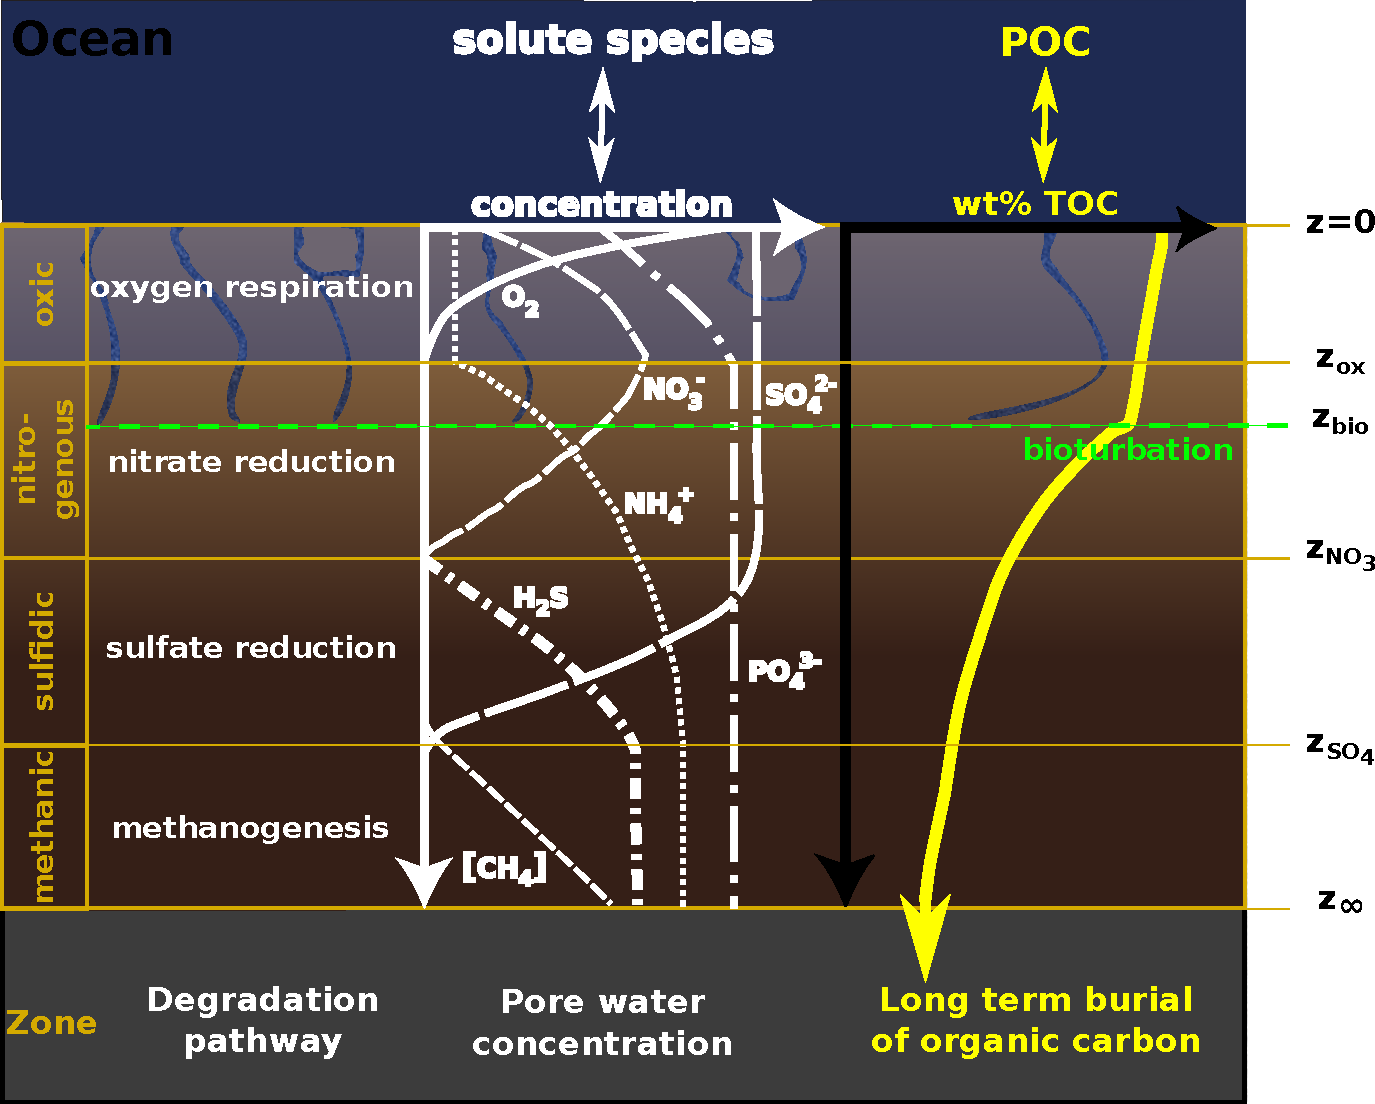
\includegraphics[width=0.8\textwidth]{figures/Sediment-model-with-profiles.pdf}
	\caption{Schematic of the different modelled species and zones in OMEN-SED. Here showing the case $z_{\mathrm{ox}} < z_{\mathrm{bio}} < z_{\chem{NO_3}} < z_{\chem{SO_4}}$.}
	\label{fig:Sediment_layers}
	\end{center}
\end{figure}

OMEN-SED accounts for both the advective, as well as the diffusive transport of dissolved and solid species. Solid and dissolved species are buried in the sediment according to a constant burial rate $w$, thus 
neglecting the effect of sediment compaction (i.e. $\frac{\partial \phi}{\partial z}=0$) due to mathematical constraints. 
The molecular diffusion of dissolved species is described by Fick's law applying a species-specific apparent diffusion coefficient, $D_{\mathrm{mol},i}$.  In addition, the activity of infaunal organisms in the bioturbated zone 
is simulated using a diffusive term \citep[e.g.][]{boudreau_mathematics_1986}, with a constant bioturbation coefficient $D_{\mathrm{bio}}$ in the bioturbated zone, 
while $D_{\mathrm{bio}}$ is set to zero below the maximum bioturbation depth, $z_{bio}$. 
The pumping activity by burrow-dwelling animals and the resulting ventilation of tubes, the so-called bioirrigation, is encapsulated in a factor $f_{ir}$ that enhances the molecular diffusion coefficient 
\citep[hence, $D_{i,0}=D_{\mathrm{mol},i}\cdot f_{ir}$,][]{soetaert_model_1996}. 
% The flux divergence is thus given by:
% \begin{equation}
% \frac{\partial F}{\partial z}=-\frac{\partial}{\partial z}\left( -\xi D_i \frac{\partial C_i}{\partial z} +\xi w C_i\right) \label{Eq_flux_divergence}
% \end{equation}
% where $D_i$ is the apparent diffusion coefficient of species $i$ ($D_i=D_{i,0}+D_{\mathrm{bio}}=D_{\mathrm{mol},i}\cdot f_{ir}+D_{\mathrm{bio}}$ for dissolved species and $D_i=D_{\mathrm{bio}}$ for solid species) and $w$ is the 
% burial rate.
The reaction network of OMEN-SED accounts for the most important primary and secondary redox reactions, equilibrium reactions, mineral dissolution and precipitation, as well as adsorption and desorption processes that affect 
the dissolved and solid species explicitly resolved in OMEN-SED. Tables \ref{table:reactions_processes} and \ref{table:Reaction_Network} provide a summary of the reactions and biogeochemical tracers considered in OMEN-SED together 
with their respective reaction stoichiometries. %Table \ref{table:Reaction_Network} summarises their reaction stoichiometry and Table \ref{table:ReactionOverview} provides an overview of their description in the model.
% %>>>
% \marginnote{\textbf{SA:} Tab 1 is maybe a bit redundant? \textbf{DH:} I still think it's a good summary/overview!? and the other one could go into the appendix!?}[-1.5cm]%<<<

\begin{table}[tbp]
\caption{Reactions and biogeochemical tracers implemented in the reaction network of OMEN-SED. The primary and secondary redox reactions are listed in the sequence they occur with increasing sediment depth.}
% title of Table
\centering
% used for centering table
\begin{tabular}{l l}
% centered columns (6 columns)
\hline\hline
%inserts double horizontal lines
 & Description\\
\hline
Primary redox reactions &  Degradation of organic matter via aerobic degradation, denitrification,\\
& sulfate reduction, methanogenesis (implicit)\\
Secondary redox reactions &  Oxidation of ammonium and sulfide by oxygen, anaerobic oxidation\\
& of methane by sulfate\\
Adsorption/Desorption & Ad-/Desorption of P on/from \chem{Fe(OH)_3}, \chem{NH_4} adsorption, \chem{PO_4} adsorption\\ %\textcolor{red}{Formation of Fe-bound P, reduction of Fe oxides (?correct here)},\\
Mineral precipitation & Formation of authigenic P \\
Biogeochemical tracers & Organic matter (2-G), oxygen, nitrate, ammonium, sulfate, sulfide (hydrogen sulfide),\\
&  phosphate, Fe-bound P, DIC, ALK\\
\hline\hline
% inserts double horizontal lines
\end{tabular}
\label{table:reactions_processes}
% is used to refer this table in the text

\end{table}
 
All parameters in Eq. (\ref{eq:Eq_generaldiagenetic}) may vary with depth and many reaction rate expressions depend on the concentration of other species. 
Expressing Eq. (\ref{eq:Eq_generaldiagenetic}) for a set of chemical species thus results in a non-linear, coupled set of equations that can only 
be solved numerically. 
However, OMEN-SED is designed for the coupling to Earth system models and, therefore, cannot afford a computationally expensive numerical solution. 
Yet, a computationally efficient analytical solution of Eq. (\ref{eq:Eq_generaldiagenetic}) can be derived by 1) assuming steady state conditions (i.e.$ \frac{\partial C_i}{\partial t}=0$) 
and 2) reducing the vertical variability in parameters and reaction rate expressions by dividing the sediment column into a number of functional 
biogeochemical zones \citep[Fig. \ref{fig:Sediment_layers}, compare e.g. ][for similar solutions]{billen1982idealized, goloway_diagenetic_1982, tromp_global_1995, gypens_simple_2008}. 
More specifically, OMEN-SED divides the sediment column into: I) a bioturbated and 
II) a non-bioturbated zone defined by an imposed, constant bioturbation depth $z_{\mathrm{bio}}$ (Fig. \ref{fig:Sediment_layers}). Furthermore, it resolves the dynamic redox stratification of marine sediments by dividing 
the sediment into 1) an oxic zone delineated by the oxygen penetration depth $z_{\mathrm{ox}}$; 2) a denitrification (or nitrogenous) zone situated between $z_{\mathrm{ox}}$ and the nitrate penetration depth $z_{\chem{NO_3}}$;
3) a sulfate reduction zone situated between $z_{\chem{NO_3}}$ and the sulfate penetration depth $z_{\chem{SO_4}}$; and 4) a methanogenic zone situated below $z_{\chem{SO_4}}$ (Fig. \ref{fig:Sediment_layers}).  
In each of these zones Eq. (\ref{eq:Eq_generaldiagenetic}) is applied with depth invariant parameters. Yet, parameter values may differ across zones. 
The biogeochemical zones are linked by stating continuity in both concentrations and fluxes at the dynamic, internal boundaries 
\citep[$z_b \in \{z_{\mathrm{bio}}, z_{\mathrm{ox}}, z_{\chem{NO_3}}, z_{\chem{SO_4}} \}$, compare e.g.][]{billen1982idealized, ruardij_benthic_1995}. These boundaries are dynamic because their depth varies in response to changing ocean 
boundary conditions and forcings (see Section \ref{subsec:GBCM} for details). Furthermore, the maximum bioturbation depth is not restricted to a specific biogeochemical zone, 
hence OMEN-SED allows bioturbation to occur in the anoxic zones of the sediment (here all zones $z > z_{\mathrm{ox}}$ combined). 
In addition, the formulation of the reaction term in Eq. (\ref{eq:Eq_generaldiagenetic}) varies between zones and encapsulates the most pertinent reaction 
processes within the respective zone (see Section \ref{subsec:ReactionNetwork}), thus simplifying the mathematical description of the reaction network while 
retaining most of its biogeochemical complexity.

All consumption or production processes of dissolved species related to the degradation of organic matter are a function of the organic matter concentration and, 
because first-order decay is assumed in the kinetic expression, can  be expressed 
as a series of exponential terms ($ \sum_j \alpha_j \exp(-\beta_j z)$, see Eq. (\ref{eq:generalODE})). In addition, slow adsorption/desorption and mineral precipitation 
processes can be expressed as zero or first order (reversible) reaction ($Q$ or $k\cdot (C_i - \tilde{C})$, in Eq. (\ref{eq:generalODE})). 
Fast adsorption is described as an instantaneous equilibrium reaction using a constant adsorption coefficient $K_i$. 
The reoxidation of reduced substances is accounted for implicitly by adding a (consumption/production) flux to the internal boundary conditions 
(see Sections \ref{subsubsec:O2}, \ref{subsubsec:N} and \ref{subsubsec:S} \textbf{SA: make reference to the section where this is explained in detail}). 
%>>>
\marginnote{\textbf{DH}: Do you mean these sections? Not discussed in further details anywhere else}[-1.5cm]%<<<
%>>>
This simplification has been used previously by \citet{gypens_simple_2008} for nitrate and ammonium and can be justified as it has been shown that the 
reoxidation mainly occurs within a thin layer at the oxic/anoxic interface \citep{soetaert_model_1996}. 
The general reaction-transport equation of OMEN-SED is thus given by:
\begin{empheq}[box={\mybluebox[5pt]}]{equation}
  \frac{\partial C_i}{\partial t} = 0 = \frac{D_i}{1+K_i}\frac{\partial^2C_i }{\partial z^2} - w\frac{\partial C_i }{\partial z} - \frac{1}{1+K_i} \left(  \sum_j \alpha_j \exp(-\beta_j z) + \sum_l k_l \cdot C_i - \sum_m Q_m \right) \label{eq:generalODE}
\end{empheq}
% \begin{equation} 
%  \boxed{\frac{\partial C_i}{\partial t} = 0 = D_i\frac{\partial^2C_i }{\partial z^2} - w\frac{\partial C_i }{\partial z} - k\cdot C_i - \sum_j \alpha_j \exp(-\beta_j z) + Q} \label{eq:generalODE_orig}
%  \end{equation}
where $1/\beta_j$ can be interpreted as the length scale and $\alpha_j$ as the relative importance (or the magnitude at $z = 0$) of reaction $j$ \citep{boudreau1997diagenetic}, 
$k_l$ are generic first order reaction rate constants and $Q_m$ are zeroth-order (or constant) reaction rates.

The analytical solution of Eq. (\ref{eq:generalODE}) is of the general form:
\begin{align}
 C_i(z) &= A \exp(az) + B  \exp(bz) + \sum_j \frac{\alpha_j}{D \beta_j^2-w\beta_j- \sum_l k_l}\cdot \exp(-\beta_j z) + \frac{\sum_m Q_m}{\sum_l k_l} \label{eq:ODE_general_solution_generalapproach}
\end{align}
with 
\begin{equation} 
 a = \frac{w - \sqrt{w^2+4\cdot D\cdot \sum_l k_l}}{2\cdot D}, \quad b = \frac{w + \sqrt{w^2+4\cdot D\cdot \sum_l k_l}}{2\cdot D}
\end{equation}
where $A$ and $B$ are integration constants that can be determined by applying a set of internal boundary conditions (see Section \ref{subsec:Determine_IC}).
% %>>>
% \marginnote{\textbf{DH}: Should it be $D \beta_i^2+w\beta_i-k$ in the denom. - see \citet{boudreau1997diagenetic} Exp 6-13 Eq. 6.121}[-1.5cm]%<<<
% %>>>

Based on Eq. (\ref{eq:generalODE}) and its analytical solution Eq. (\ref{eq:ODE_general_solution_generalapproach}), OMEN-SED returns the fraction of particulate organic carbon (POC) buried in the sediment, 
$f_{\mathrm{POC}}$, as well as the benthic uptake/return fluxes $F_{C_i}$ of dissolved species $C_i$ (in mol cm$^{-2}$ year$^{-1}$) in response to changing boundary conditions and forcings:
\begin{align}
f_{\mathrm{POC}} &= \frac{\mathrm{POC}(z_\infty)}{\mathrm{POC}(0)} \label{f_POC_pres}\\
F_{C_i} &= \phi(0) \left(D_i \frac{\partial C_i(z)}{\partial z}\bigg\rvert_{z=0} - w \cdot C_i(0) \right) \label{Eq:F_Ci_SWIflux}
\end{align}
where $w$ is the deposition rate, $D_i$ is the diffusion coefficient and $\mathrm{POC}(0)$, $\mathrm{POC}(z_\infty)$, $C_i(0)$ denotes the concentration of POC and dissolved species $i$ at the SWI and 
at the lower sediment boundary, respectively.


\subsection{Conservation Equations and Analytical Solution}\label{subsec:ReactionNetwork}

\subsubsection{Organic matter or Particulate Organic Carbon (POC)}\label{subsubsec:OM}
In marine sediments, particulate organic carbon (POC) is degraded by heterotrophic activity coupled to the sequential utilisation of terminal electron acceptors according to the free energy gain of the half-reaction 
\citep[$\chem{O_2} > \chem{NO_3^-}> \chem{MnO_2} > \chem{Fe(OH)_3} > \chem{SO_4^{2-}}$, e.g.][]{stumm_aquatic_2012}. 
Here, organic matter degradation is described via a multi G-model approach \citep[][and references therein]{arndt_quantifying_2013}, 
dividing the bulk OM into a number $i$ of discrete compound classes $\chem{POC}_i$ characterised by class-specific first-order degradation rate constants $k_i$. 
The conservation equation for organic matter dynamics is thus given by:
\begin{equation}
 \frac{\partial \chem{POC}_i}{\partial t} = 0= D_{\chem{POC}_i} \frac{\partial^2\chem{POC}_i }{\partial z^2} - w\frac{\partial \chem{POC}_i }{\partial z} - k_i\cdot \chem{POC}_{i} \label{eq:ODE_OC}
\end{equation}
% where:
% \begin{align}
%  D_{C_i}&=D_{\mathrm{bio}} 	 &\text{if ($z\leq z_{\mathrm{bio}}$)}\\
%  D_{C_i}&=0            &\text{if ($z > z_{\mathrm{bio}}$)} 
% \end{align}
with $D_{\chem{POC}_i}=D_{\mathrm{bio}}$ for $z\leq z_{\mathrm{bio}}$ and $D_{\chem{POC}_i}=0$ for $z > z_{\mathrm{bio}}$. 
Integration of equations \eqref{eq:ODE_OC} yields the following general solutions:
\begin{align}
\intertext{I. Bioturbated zone ($z\leq z_{bio}$)}
 \chem{POC}_{i}^I(z) &= A_{1i}\cdot exp(a_{1i} z)+B_{1i}\cdot exp(b_{1i} z) \notag\\% \qquad &\text{1. Layer: ($z\leqq z_{bio}$)} \notag\\
 \intertext{which using the boundary condition at z = 0 can be rewritten as:}
 \chem{POC}_{i}^I(z) &\overset{\mathrm{BC 1)}}{=} A_{1i}\cdot [ exp(a_{1i} z)-exp(b_{1i} z)] +\chem{POC}_{0i}\cdot exp(b_{1i} z) \label{eq:GS_OM1}
\intertext{II. Non-bioturbated zone ($z_{bio} < z$)}
 \chem{POC}_{i}^{II}(z) &= A_{2i}\cdot exp(a_{2i} z) \label{eq:GS_OM2}%  &\text{2. Layer: ($z> z_{bio}$)} \label{eq:GS_OM2} 
\end{align}
where
\begin{equation} 
 a_{1i} = \frac{w - \sqrt{w^2+4\cdot D_{\chem{POC}_i}\cdot k_i}}{2\cdot D_{\chem{POC}_i}}, \quad b_{1i} = \frac{w + \sqrt{w^2+4\cdot D_{\chem{POC}_i}\cdot k_i}}{\cdot 2D_{\chem{POC}_i}}, \quad a_{2i} = -\frac{k_i}{w}
\end{equation}
Determining the integration constants ($A_{1,i},\ B_{1,i},\ A_{2,i}$) requires the definition of a set of boundary conditions (Table \ref{Tab:BC_OM}). 
For organic matter, OMEN-SED applies a known concentration/flux at the sediment-water interface and assumes continuity across the bottom of the bioturbated zone, $z_{\mathrm{bio}}$. 
See Section \ref{subsec:GBCM} for further details on how to find the analytical solution.

\begin{table}[tbp]
\caption{OM Boundary conditions applied in OMEN-SED. For the boundaries we define:  $z_{\mathrm{bio}}^- := \lim_{h\to0} (z_{\mathrm{bio}}-h)$ and $z_{\mathrm{bio}}^+ := \lim_{h\to0} (z_{\mathrm{bio}}+h)$.}
% title of Table
\centering
% used for centering table
\begin{tabular}{ |c| l| c l|}
\hline
\textbf{Boundary}& \textbf{Condition}& &\\
\hline
$z=0$& known concentration& 1)& $\chem{POC}_i(0)=\chem{POC}_{0i}$\\
$z=z_{\mathrm{bio}}$&continuity& 2)& $\chem{POC}_i(z_{\mathrm{bio}}^-)$=$\chem{POC}_i(z_{\mathrm{bio}}^+)$\\
               &&3)&$-D_{\mathrm{bio}}\cdot \frac{\partial \chem{POC}_i}{\partial z}|_{z_{\mathrm{bio}}^-}=0$\\
%Dom was               &&3) $D_{\mathrm{bio}}\cdot \frac{\partial \chem{POC}_i}{\partial z}|_{z_{\mathrm{bio}}^-}-w\cdot \chem{POC}_i(z_{\mathrm{bio}}^-)=-w\cdot \chem{POC}_i(z_{\mathrm{bio}}^+)$\\
\hline
\end{tabular}
\label{Tab:BC_OM}
\end{table}


\subsubsection{Oxygen}\label{subsubsec:O2}
OMEN-SED explicitly accounts for oxygen consumption by the aerobic degradation of organic matter within the oxic zone, as well as the oxidation of reduced species (i.e. \chem{NH_4}, \chem{H_2S}) 
produced in the anoxic zones of the sediment. 
In the oxic zone ($z<z_{ox}$), the aerobic degradation consumes oxygen with a fixed \chem{O_2:C} ratio (\chem{O_2C}, Tab. \ref{table:reaction_parameters}). 
A predefined fraction, $\gamma_\chem{NH_4}$, of the ammonium produced during the aerobic degradation of OM is nitrified to nitrate, consuming two moles of oxygen per mole of ammonium produced. 
In addition, OMEN-SED implicitly accounts for the oxygen consumption due to oxidation of reduced species (\chem{NH_4}, \chem{H_2S}) produced below the oxic zone through the flux boundary condition at the dynamically calculated 
(see section \ref{subsubsec:Stoich_reaction_params} for details) oxygen penetration depth $z_{\mathrm{ox}}$. 
%This simplification can be justified as it has been shown that these secondary redox reactions mainly occur at the oxic/anoxic interface \citep{soetaert_model_1996}. 
All oxygen consumption processes can thus be formulated as a function of organic matter degradation. 
The conservation equation for oxygen is given by: \textbf{SA: I'd show the POC substitution in the equations below}:
%>>>
\marginnote{\textbf{DH}: you mean the way I did it or in the solution? I think it's easier to understand (also how to get the solution) if it's done in the ODE}[-0.5cm]%<<<

\begin{align} 
 \frac{\partial \chem{O_2}}{\partial t} = 0 &= D_{\chem{ \chem{O_2}}}\frac{\partial^2  \chem{O_2} }{\partial z^2} - w\frac{\partial  \chem{O_2}}{\partial z} - \frac{1-\phi}{\phi}\sum_i k_i \cdot [ \chem{O_2C} + 2 \gamma_{\chem{NH_4}} \chem{NC_i} ]\cdot \chem{POC}_{i}(z) \label{eq:ODE_O2_1}
\intertext{which, using Eq. (\ref{eq:GS_OM1}) and (\ref{eq:GS_OM2}) for the depth-distribution of \chem{POC_i(z)}, can be written as:}
\intertext{I Bioturbated zone ($z\leq z_{\mathrm{bio}}$)}
 \frac{\partial \chem{O_2^I}}{\partial t} &= 0 \overset{\ref{eq:GS_OM1}}{=} D^{I}_{\chem{ \chem{O_2}}}\frac{\partial^2  \chem{O_2} }{\partial z^2} - w\frac{\partial  \chem{O_2}}{\partial z} \notag\\
 &\quad - \frac{1-\phi}{\phi}\sum_i k_i \cdot [ \chem{O_2C} + 2 \gamma_{\chem{NH_4}} \chem{NC_i} ]\cdot  \bigl\lgroup A_{1i}\cdot [ exp(a_{1i} z)-exp(b_{1i} z)] +\chem{POC}_{0i}\cdot exp(b_{1i} z) \bigr\rgroup\notag
\intertext{II Non-bioturbated zone ($z_{\mathrm{bio}} < z < z_{\mathrm{ox}}$)}
\frac{\partial \chem{O_2}^{II}}{\partial t} &=0 \overset{\ref{eq:GS_OM2}}{=} D^{II}_{\chem{ \chem{O_2}}}\frac{\partial^2  \chem{O_2} }{\partial z^2} - w\frac{\partial  \chem{O_2}}{\partial z} - \frac{1-\phi}{\phi}\sum_i k_i \cdot [ \chem{O_2C} + 2 \gamma_{\chem{NH_4}} \chem{NC_i} ]\cdot \bigl\lgroup A_{2i}\cdot exp(a_{2i} z)  \bigr\rgroup\notag
\end{align}
where $D^I_{\chem{ \chem{O_2}}}$ and $D^{II}_{\chem{ \chem{O_2}}}$ denote the \chem{O_2} diffusion coefficient for the bioturbated and non-bioturbated zone, respectively. 
The term $\frac{1-\phi}{\phi}$ accounts for the volume conversion from solid to dissolved phase and \chem{NC_i} is the nitrogen to carbon ratio in OM. 
%\textbf{SA: explain all terms}\\
% %>>>
%\marginnote{\textbf{DH}: Other terms are explained earlier in \ref{subsubsec:O2} or \ref{subsubsec:OM}}[-0.5cm]%<<<
Integration yields the following analytical solution for each zone: 
\begin{align}
\intertext{I Bioturbated zone ($z\leq z_{\mathrm{bio}}$):}
\chem{O_2}^I(z) &= A_{\chem{O_2}}^1 + B_{\chem{O_2}}^1 \cdot \exp(b_{\chem{O_2}}^1 z) + \sum_i\Phi_{1,i}^I \cdot \exp(a_{1i}z)+  \sum_i\Phi_{1,i}^{II}\cdot \exp(b_{1i}z) +  \sum_i\Phi_{1,i}^{III} \cdot \exp(b_{1i}z)
\intertext{II Non-bioturbated zone ($z_{\mathrm{bio}} < z < z_{\mathrm{ox}}$)}
\chem{O_2}^{II}(z) &= A_{\chem{O_2}}^2 + B_{\chem{O_2}}^2 \cdot \exp(b_{\chem{O_2}}^2 z) + \sum_i\Phi_{i,2}^I \cdot \exp(a_{2i}z)
\end{align}
with 
\begin{align}
%&b_{O_2}^1 = \frac{w + \sqrt{w^2+4D_{O_2}^{I}\cdot k_{O_2}}}{2D_{O_2}^{I}} = \frac{w}{D_{O_2}^{I}}, \quad b_{O_2}^2 = \frac{w}{D_{O_2}^{II}}\notag\\
&b_{\chem{O_2}}^1 = \frac{w}{D_{\chem{O_2}}^{I}}, \quad b_{\chem{O_2}}^2 = \frac{w}{D_{\chem{O_2}}^{II}}\notag\\
&\Phi_{1,i}^I = \frac{1-\phi}{\phi}\cdot\frac{k_i\cdot(\chem{O_2C}+2 \gamma_{\chem{NH_4}} \chem{NC_i})\cdot A_{1i}}{D_{\chem{O_2}}^{I}(-a_{1i})^2-w\cdot (-a_{1i})}, &\Phi_{1,i}^{II} = - \frac{1-\phi}{\phi}\cdot\frac{k_i\cdot(\chem{O_2C}+2 \gamma_{\chem{NH_4}} \chem{NC_i})\cdot A_{1i}}{D_{\chem{O_2}}^{I}(-b_{1i})^2-w\cdot (-b_{1i})}\notag\\
&\Phi_{1,i}^{III} = \frac{1-\phi}{\phi}\cdot\frac{k_i\cdot(\chem{O_2C}+2 \gamma_{\chem{NH_4}} \chem{NC_i})\cdot \chem{POC}_{0i}}{D_{\chem{O_2}}^{I}(-b_{1i})^2-w\cdot (-b_{1i})} \notag\\
&\Phi_{i,2}^I := \frac{1-\phi}{\phi}\cdot\frac{k_i\cdot(\chem{O_2C}+2 \gamma_{\chem{NH_4}} \chem{NC_i})\cdot A_{2i}}{D_{\chem{O_2}}^{II}(-a_{2i})^2-w\cdot (-a_{2i})} \notag
\end{align}

Determining the four integration constants ($A_{\chem{O_2}}^1,\, B_{\chem{O_2}}^1,\, A_{\chem{O_2}}^2,\, B_{\chem{O_2}}^2$, see Section \ref{subsec:Determine_IC} for details), as well as the $a-priori$ unknown oxygen penetration 
depth requires the definition of five boundary conditions (see Table \ref{Tab:BC_O2}). 
At the sediment-water interface, OMEN-SED applies a Dirichlet condition (i.e. known concentration) and assumes concentration and flux continuity across the bottom of the bioturbated zone, $z_{\mathrm{bio}}$. 
The oxygen penetration depth $z_{\mathrm{ox}}$ marks the lower boundary and is dynamically calculated as the depth at which $\chem{O_2}(z)=0$. 
Therefore, OMEN-SED applies a Dirichlet boundary condition $\chem{O_2}(z_{\mathrm{ox}})=0$. In addition, a flux boundary is applied that implicitly accounts for the oxygen consumption by the partial oxidation 
of $\chem{NH_4}$ and $\chem{H_2S}$ diffusing into the oxic zone from below (BC 4.2, Table \ref{Tab:BC_O2}). It is assumed that respective fractions ($\gamma_{\chem{NH_4}}$ and $\gamma_{\chem{H_2S}}$) are directly reoxidised 
at the oxic/anoxic interface and the remaining fraction escapes reoxidation. OMEN-SED iteratively solves for $z_{\mathrm{ox}}$ by first testing if there is oxygen left at $z_\infty$ (i.e. $\chem{O_2}(z_\infty) > 0$) and, otherwise, by finding the root for the flux 
boundary condition 4.2 (Table \ref{Tab:BC_O2}). If $z_{\mathrm{ox}}=z_\infty$,  a zero diffusive flux boundary condition is applied as lower boundary condition. 
%>>>
\marginnote{\textbf{DH}: Edited explanation of finding $z_{ox}$}[-1.5cm]%<<<

\begin{table}[tbp]
\caption{Boundary conditions for oxygen. For the boundaries we define:  $z_{\mathrm{bio}}^- := \lim_{h\to0} (z_{\mathrm{bio}}-h)$ and $z_{\mathrm{bio}}^+ := \lim_{h\to0} (z_{\mathrm{bio}}+h)$.}
% title of Table
\centering
% used for centering table
\begin{tabular}{ |c| l| c l|}
\hline
\textbf{Boundary}& \textbf{Condition}& &\\
\hline
$z=0$& known concentration& 1)&$\chem{O_2}(0)=O_{20}$\\
$z=z_{\mathrm{bio}}$&continuity& 2)&$ \chem{O_2}(z_{\mathrm{bio}}^-)$=$ \chem{O_2}(z_{\mathrm{bio}}^+)$\\
               &&3)&$-\left(D_{ \chem{O_2},0}+D_{\mathrm{bio}}\right )\cdot \frac{\partial  \chem{O_2}}{\partial z}|_{z_{\mathrm{bio}}^-}=-D_{\chem{O_2},0} \cdot \frac{\partial  \chem{O_2}}{\partial z}|_{z_{\mathrm{bio}}^+}$\\
%Dom was               &&3) $\left(D_{\mathrm{bio}}+D_{mol, \chem{O_2}}\right )\cdot \frac{\partial  \chem{O_2}}{\partial z}|_{z_{\mathrm{bio}}^-}-w\cdot  \chem{O_2}(z_{\mathrm{bio}}^-)=D_{mol, \chem{O_2}} \cdot \frac{\partial  \chem{O_2}}{\partial z}|_{z_{\mathrm{bio}}^+}-w\cdot  \chem{O_2}(z_{\mathrm{bio}}^+)$\\
$z=z_{\mathrm{ox}}$&  \chem{O_2} consumption & 4)&\textbf{IF} $ (\chem{O_2}(z_\infty)> 0 )$\\
& ($z_{\mathrm{ox}} = z_\infty$) & 4.1)&\quad $\frac{\partial  \chem{O_2}}{\partial z}|_{z_{\mathrm{ox}}}=0$ \\
& & &\textbf{ELSE} \\
& ($z_{\mathrm{ox}} < z_\infty$) & 4.2) &\quad $  \chem{O_2}(z_{\mathrm{ox}})=0$  \quad and \quad $-D_{ \chem{O_2}} \cdot \frac{\partial  \chem{O_2}}{\partial z}|_{z_{\mathrm{ox}}}=F_{red}(z_\mathrm{ox})$\\
%$z=z_{\mathrm{ox}}$& & 5) $-D_{ \chem{O_2}} \cdot \frac{\partial  \chem{O_2}}{\partial z}|_{z_{\mathrm{ox}}}=F_{red, z_{\mathrm{ox}}}$\\   
& with &&$\quad F_{red}(z_\mathrm{ox})=\frac{1-\phi}{\phi} \cdot \int_{\tilde{z}_{\chem{NO_3}}}^{\infty}  \sum_i \left( 2\gamma_{\chem{NH_4}} \chem{NC_i} + 2\gamma_{\chem{H_2S}} \chem{SO_4C} \right) k_i \chem{POC}_i\ dz$ \\
% was from Sandra &with:&$F_{red,z_{\mathrm{ox}}}=\beta \cdot \int_{z_{\mathrm{ox}}}^{\inf}  \sum_i k_i\cdot \chem{POC}_i  dz  + 2\cdot \gamma \cdot \int_{z_{\mathrm{ox}}}^{\inf}  \sum_i k_i\cdot \chem{POC}_i  -  $ \\
\hline  
\multicolumn{4}{l}{Note: $\tilde{z}_{\chem{NO_3}} = z_{\mathrm{ox}}$ as upper boundary here, as $z_{\chem{NO_3}}$ is not known at this point.}\\
\end{tabular}
\label{Tab:BC_O2}
% is used to refer this table in the text
\end{table}

\subsubsection{Nitrate and Ammonium}\label{subsubsec:N}
Nitrogen dynamics in OMEN-SED are controlled by the metabolic production of ammonium, nitrification, denitrification as well as ammonium adsorption. 
Ammonium is produced by organic matter degradation in both the oxic and anoxic zones, while denitrification consumes nitrate in the denitrification zone with a fixed \chem{NO_3:C} ratio (\chem{NO_3C}, Tab. \ref{table:reaction_parameters}) \textbf{SA: need explanation}. 
%>>>
\marginnote{\textbf{DH}: explanation sufficient?}[-0.5cm]%<<<
The adsorption of ammonium to sediment particles is formulated as an equilibrium process with constant equilibrium adsorption coefficient $K_\chem{NH_4}$, thus assuming that the adsorption is fast compared with the 
characteristic time scales of transport processes \citep{wang_multicomponent_1996}. In addition, a defined fraction, $\gamma_{\chem{NH_4}}$, of metabolically produced ammonium is directly nitrified to nitrate in the oxic zone, 
while the nitrification of upward diffusing ammonium produced in the sulfidic and methanic zones is implicitly accounted for in the boundary conditions. The conservation equations for ammonium and nitrate are thus given by:

\begin{align}
\intertext{1. Oxic zone ($z \leq z_{\mathrm{ox}}$)}
 \frac{\partial \chem{NO_3}^I}{\partial t} &= 0 = D_\chem{NO_3} \frac{\partial^2\chem{NO_3}^I }{\partial z^2} - w\frac{\partial \chem{NO_3}^I }{\partial z} + \gamma_{\chem{NH_4}} \frac{1-\phi}{\phi} \cdot \sum_i \chem{NC_i} \cdot k_i \cdot \chem{POC}_{i}(z)\label{eq:NO3_ODE1_L1}\\ %\qquad &\text{1. Layer ($z\leq z_{\mathrm{ox}}$)}\\
 \frac{\partial \chem{NH_4}^I}{\partial t} &= 0 = \frac{D_{\chem{NH_4}}}{1+K_\chem{NH_4}} \frac{\partial^2\chem{NH_4}^I }{\partial z^2} - w\frac{\partial \chem{NH_4}^I }{\partial z} + \frac{1-\gamma_{\chem{NH_4}}}{1+K_\chem{NH_4}}\cdot \frac{1-\phi}{\phi} \cdot \sum_i \chem{NC_i} \cdot k_i \cdot \chem{POC}_{i}(z)\label{eq:NH4_ODE1_L1}\\
 \intertext{2. Denitrification (or nitrogenous) zone ($z_{\mathrm{ox}} < z \leq z_{\chem{NO_3}}$)} 
\frac{\partial \chem{NO_3}^{II}}{\partial t} &= 0 = D_{\chem{NO_3}} \frac{\partial^2\chem{NO_3}^{II} }{\partial z^2} - w\frac{\partial \chem{NO_3}^{II} }{\partial z} - \frac{1-\phi}{\phi} \chem{NO_3C} \cdot \sum_i k_i \cdot \chem{POC}_{i}(z) \label{eq:NO3_ODE1_L2}\\
\frac{\partial \chem{NH_4}^{II}}{\partial t} &= 0 = \frac{D_{\chem{NH_4}}}{1+K_\chem{NH_4}} \frac{\partial^2\chem{NH_4}^{II} }{\partial z^2} - w\frac{\partial \chem{NH_4}^{II} }{\partial z} \label{eq:NH4_ODE1_L2}
 \intertext{3. Sulfidic and methanic zone ($z_{\chem{NO_3}} < z \leq z_\infty$)} 
\frac{\partial \chem{NH_4}^{III}}{\partial t} &= 0 = \frac{D_{\chem{NH_4}}}{1+K_\chem{NH_4}} \frac{\partial^2\chem{NH_4}^{III} }{\partial z^2} - w\frac{\partial \chem{NH_4}^{III} }{\partial z} + \frac{1}{1+K_\chem{NH_4}}\cdot\frac{1-\phi}{\phi} \cdot \sum_i \chem{NC_i} \cdot k_i \cdot \chem{POC}_{i}(z)\label{eq:NH4_ODE1_L3}
\end{align}

where $D_\chem{NO_3}$ and $D_{\chem{NH_4}}$ denote the diffusion coefficients for \chem{NO_3} and \chem{NH_4} which depend on the bioturbation status of the respective geochemical zone (compare Section \ref{subsec:GBCM}). 
% %>>>
% \marginnote{\textbf{DH}: all other params explained earlier}[-0.5cm]%<<<
Integration of Eq. (\ref{eq:NO3_ODE1_L1}) - (\ref{eq:NH4_ODE1_L3}) yields the analytical solutions, which are not further developed here but follow the procedure outlined in Section \ref{subsubsec:O2} for oxygen 
(also see Section \ref{subsec:GBCM} for more details on how to find the analytical solution). Table \ref{Tab:BC_NO3+NH4} summarises the boundary conditions applied in OMEN-SED to solve Eq. (\ref{eq:NO3_ODE1_L1}) - (\ref{eq:NH4_ODE1_L3}) 
and to find the $a-priori$ unknown nitrate penetration depth, $z_\chem{NO_3}$. 
The model assumes known bottom water concentrations for both \chem{NO_3} and \chem{NH_4}, the complete consumption of nitrate at the nitrate penetration depth (in case  $z_{\chem{NO_3}} < z_\infty$) and no change in %nitrate and 
ammonium flux at $z_\infty$. In addition, concentration and diffusive flux continuity across $z_{\mathrm{bio}}$ and $z_{\mathrm{ox}}$ is considered for \chem{NO_3} and \chem{NH_4}. 
Furthermore, the reoxidation of upward-diffusing reduced ammonium is accounted for in the oxic-anoxic boundary condition for nitrate and ammonium. 
OMEN-SED iteratively solves for $z_{\chem{NO_3}}$ by first testing if there is nitrate left at $z_\infty$ (i.e. $\chem{NO_3}(z_\infty) > 0$) and, otherwise, by finding the root for the flux 
boundary condition 6.2 (Table \ref{Tab:BC_NO3+NH4}).

\begin{table}[tbp]
\caption{Boundary conditions for nitrate and ammonium. For the boundaries we define:  $z^-_{\_\_} := \lim_{h\to0} (z_{\_\_}-h)$ and $z^+_{\_\_} := \lim_{h\to0} (z_{\_\_}+h)$.}
% title of Table
\centering
% used for centering table
\begin{tabular}{ |c| c| c l|}
\hline
\textbf{Boundary}& \textbf{Condition}& &\\
\hline
$z=0$& known concentration& 1)& $\chem{NO_3}(0)=\chem{NO_{30}}$  \\
$z=z_{\mathrm{bio}}$&continuity& 2)& $\chem{NO_3}(z_{\mathrm{bio}}^-)$=$\chem{NO_3}(z_{\mathrm{bio}}^+)$\\
               && 3)& $-\left(D_{\chem{NO_3},0}+D_{\mathrm{bio}}\right )\cdot \frac{\partial \chem{NO_3}}{\partial z}|_{z_{\mathrm{bio}}^-}=-D_{\chem{NO_3},0} \cdot \frac{\partial \chem{NO_3}}{\partial z}|_{z_{\mathrm{bio}}^+}$\\
$z=z_{\mathrm{ox}}$& continuity& 4)& $\chem{NO_3}(z_{\mathrm{ox}}^-)$=$\chem{NO_3}(z_{\mathrm{ox}}^+)$\\
               && 5)& $-D_{\chem{NO_3}} \cdot \frac{\partial \chem{NO_3}}{\partial z}|_{z_{\mathrm{ox}}^-} + \gamma_{\chem{NH_4}}\cdot F_{\chem{NH_4}}(z_{\mathrm{ox}})=-D_{\chem{NO_3}} \cdot \frac{\partial \chem{NO_3}}{\partial z}|_{z_{\mathrm{ox}}^+}$\\
&where: & &$ F_{\chem{NH_4}}(z_{\mathrm{ox}})=\frac{1}{1+K_\chem{NH_4}}\cdot \frac{1-\phi}{\phi} \cdot \int_{z_{\chem{NO_3}}}^{\infty}  \sum_i \chem{NC_i} \cdot k_i \cdot \chem{POC}_i\ dz$ \\          
$z=z_{\chem{NO_3}}$& \chem{NO_3} consumption & 6) & \textbf{IF} $ (\chem{NO_3}(z_\infty)> 0 )$\\
& ($z_{\chem{NO_3}} = z_\infty$) & 6.1) & \quad $\frac{\partial \chem{NO_3}}{\partial z}|_{z_{\chem{NO_3}}}=0$\\
& & &\textbf{ELSE} \\
& ($z_{\chem{NO_3}} < z_\infty$) & 6.2) & \quad $\chem{NO_3}(z_{\chem{NO_3}})=0$  \quad and \quad $\frac{\partial  \chem{NO_3}}{\partial z}|_{z_{\chem{NO_3}}}=0$ \\
% was from Sandra &with:&$F_{red,z_{\mathrm{ox}}}=\beta \cdot \int_{z_{\mathrm{ox}}}^{\inf}  \sum_i k_i\cdot \chem{POC}_i  dz  + 2\cdot \gamma \cdot \int_{z_{\mathrm{ox}}}^{\inf}  \sum_i k_i\cdot \chem{POC}_i  -  $ \\
\hline
$z=0$& known concentration& 1)& $\chem{NH_4}(0)= \chem{NH_{40}}$  \\
$z=z_{\mathrm{bio}}$&continuity& 2)& $\chem{NH_4}(z_{\mathrm{bio}}^-)$=$\chem{NH_4}(z_{\mathrm{bio}}^+)$\\
               && 3)& $-\frac{D_{\chem{NH_4},0}+D_{\mathrm{bio}}}{1+K_\chem{NH_4}}\cdot \frac{\partial \chem{NH_4}}{\partial z}|_{z_{\mathrm{bio}}^-}=-\frac{D_{\chem{NH_4},0}}{1+K_\chem{NH_4}} \cdot \frac{\partial \chem{NH_4}}{\partial z}|_{z_{\mathrm{bio}}^+}$\\
$z=z_{\mathrm{ox}}$& continuity& 4)& $\chem{NH_4}(z_{\mathrm{ox}}^-)$=$\chem{NH_4}(z_{\mathrm{ox}}^+)$\\
  & & 5)& $-\frac{D_{\chem{NH_4}}}{1+K_\chem{NH_4}} \cdot \frac{\partial \chem{NH_4}}{\partial z}|_{z_{\mathrm{ox}}^-} -\gamma_{\chem{NH_4}}\cdot F_{\chem{NH_4}}(z_{\mathrm{ox}})=-\frac{D_{\chem{NH_4}}}{1+K_\chem{NH_4}} \cdot \frac{\partial \chem{NH_4}}{\partial z}|_{z_{\mathrm{ox}}^+}$\\
&where: & & $F_{\chem{NH_4}}(z_{\mathrm{ox}})=\frac{1}{1+K_\chem{NH_4}}\cdot \frac{1-\phi}{\phi} \cdot \int_{z_{\chem{NO_3}}}^{\infty}  \sum_i \chem{NC_i} \cdot k_i \cdot \chem{POC}_i\ dz$ \\          
$z=z_{\chem{NO_3}}$&continuity& 6)& $\chem{NH_4}(z_{\chem{NO_3}}^-)$=$\chem{NH_4}(z_{\chem{NO_3}}^+)$\\
               & flux & 7)& $-\frac{D_{\chem{NH_4}}}{1+K_\chem{NH_4}}\cdot \frac{\partial \chem{NH_4}}{\partial z}|_{z_{\chem{NO_3}}^-}=-\frac{D_{\chem{NH_4}}}{1+K_\chem{NH_4}} \cdot \frac{\partial \chem{NH_4}}{\partial z}|_{z_{\chem{NO_3}}^+}$\\
$z=z_{\infty}$& zero \chem{NH_4} flux & 8)& $\frac{\partial \chem{NH_4}}{\partial z}|_{z_\infty}=0$\\
\hline    
\end{tabular}
\label{Tab:BC_NO3+NH4}
\end{table}


\subsubsection{Sulfate and Sulfide}\label{subsubsec:S}
Below the denitrification zone ($z>z_{\chem{NO_3}}$), organic matter degradation is coupled to sulfate reduction, consuming sulfate and producing hydrogen sulfide with a fixed \chem{SO_4:C} ratio (\chem{SO_4C}, Tab. \ref{table:reaction_parameters}). 
In addition, the anaerobic oxidation of upward diffusing methane (AOM) produced below the sulfate penetration and the associated consumption of sulfate and production of sulfide; as well as the production of sulfate and 
consumption of sulfide through sulfide oxidation are implicitly accounted for through the boundary conditions (Table \ref{Tab:BC_SO4+H2S}).
The conservation equations for sulfate and sulfide are thus given by:

\begin{align}
\intertext{1. Oxic and nitrogenous zone ($z \leq z_{\chem{NO_3}}$)}
 \frac{\partial \chem{SO_4}^I}{\partial t} &= 0 = D_{\chem{SO_4}} \frac{\partial^2\chem{SO_4}^I }{\partial z^2} - w\frac{\partial \chem{SO_4}^I }{\partial z} \label{eq:SO4_ODE1_L1}\\ %\qquad &\text{1. Layer ($z\leq z_{\mathrm{ox}}$)}\\
 \frac{\partial \chem{H_2S}^I}{\partial t} &= 0 = D_{\chem{H_2S}} \frac{\partial^2\chem{H_2S}^I }{\partial z^2} - w\frac{\partial \chem{H_2S}^I }{\partial z}\label{eq:H2S_ODE1_L1}\\
 \intertext{2.Sulfidic zone ($z_{\chem{NO_3}} < z \leq z_{\chem{SO_4}}$)} 
\frac{\partial \chem{SO_4}^{II}}{\partial t} &= 0 = D_{\chem{SO_4}} \frac{\partial^2\chem{SO_4}^{II} }{\partial z^2} - w\frac{\partial \chem{SO_4}^{II} }{\partial z} - \frac{1-\phi}{\phi} \cdot \sum_i \chem{SO_4C} \cdot k_i \cdot \chem{POC}_{i}(z) \label{eq:SO4_ODE1_L2}\\
\frac{\partial \chem{H_2S}^{II}}{\partial t} &= 0 = D_{\chem{H_2S}} \frac{\partial^2\chem{H_2S}^{II} }{\partial z^2} - w\frac{\partial \chem{H_2S}^{II} }{\partial z} + \frac{1-\phi}{\phi} \cdot \sum_i \chem{SO_4C}  \cdot k_i \cdot \chem{POC}_{i}(z)\label{eq:H2S_ODE1_L2}
 \intertext{3. Methanic zone ($z_{\chem{SO_4}} < z \leq z_{\infty}$)} 
\frac{\partial \chem{H_2S}^{III}}{\partial t} &= 0 = D_{\chem{H_2S}} \frac{\partial^2\chem{H_2S}^{III} }{\partial z^2} - w\frac{\partial \chem{H_2S}^{III} }{\partial z}\label{eq:H2S_ODE1_L3}
\end{align}
% where
% \begin{align}
%  D_{i}&=D_{i, 0}+D_{\mathrm{bio}} &\text{if ($z\leq z_{\mathrm{bio}}$)}\\
%  D_{i}&=D_{i, 0}                &\text{if ($z > z_{\mathrm{bio}}$)} 
% \end{align} 
% and $i \in \{$SO$_4$, H$_2$S$\}$. 
where $D_\chem{SO_4}$ and $D_{\chem{H_2S}}$ denote the diffusion coefficients for \chem{SO_4} and \chem{H_2S} which depend on the bioturbation status of the respective geochemical zone (compare Section \ref{subsec:GBCM}). 
Integration of Eq. (\ref{eq:SO4_ODE1_L1}) - (\ref{eq:H2S_ODE1_L3}) yields the analytical solution and Table \ref{Tab:BC_SO4+H2S} summarises the boundary conditions applied. 
OMEN-SED assumes known concentrations at the sediment-water interface and continuity across the bioturbation depth and the nitrate penetration depth. 
The reoxidation of reduced \chem{H_2S} to \chem{SO_4} is accounted for implicitly via the oxic-anoxic boundary condition for both species, while reduction of \chem{SO_4} and the associated production of \chem{H_2S} via AOM 
is accounted for through the respective boundary conditions at $z_\chem{SO_4}$. In case $z_{\chem{SO_4}}<z_\infty$, OMEN-SED assumes zero sulfate concentration at $z_{\chem{SO_4}}$ and its diffusive flux must equal the amount of 
methane produced below (with a methane to carbon ratio of \chem{MC}); or, in case $z_{\chem{SO_4}}=z_\infty$, a zero diffusive flux condition for sulfate is considered. 
OMEN-SED iteratively solves for $z_{\chem{SO_4}}$ by first testing if there is sulfate left at $z_\infty$ (i.e. $\chem{SO_4}(z_\infty) > 0$) and, otherwise, by finding the root for the flux 
boundary condition 8.2 (Table \ref{Tab:BC_SO4+H2S}). At the lower boundary $z_\infty$ zero diffusive flux of \chem{H_2S} is considered. 


\begin{table}[tbp]
\caption{Boundary conditions for sulfate and sulfide. For the boundaries we define:  $z^-_{\_\_} := \lim_{h\to0} (z_{\_\_}-h)$ and $z^+_{\_\_} := \lim_{h\to0} (z_{\_\_}+h)$.}
% title of Table
\centering
% used for centering table
\hspace*{-1cm}\begin{tabular}{ |c| c| c l|}
\hline
\textbf{Boundary}& \textbf{Condition}&&\\
\hline
$z=0$& known concentration& 1)& \chem{SO_4}(0)=\chem{SO_{40}}  \\
$z=z_{\mathrm{bio}}$&continuity& 2)& $\chem{SO_4}(z_{\mathrm{bio}}^-)$=$\chem{SO_4}(z_{\mathrm{bio}}^+)$\\
               & flux & 3)& $-\left(D_{\chem{SO_4},0}+D_{\mathrm{bio}}\right )\cdot \frac{\partial \chem{SO_4}}{\partial z}|_{z_{\mathrm{bio}}^-}=-D_{\chem{SO_4},0} \cdot \frac{\partial \chem{SO_4}}{\partial z}|_{z_{\mathrm{bio}}^+}$\\
$z=z_{\mathrm{ox}}$& continuity& 4)& $\chem{SO_4}(z_{\mathrm{ox}}^-)$=$\chem{SO_4}(z_{\mathrm{ox}}^+)$\\
               & flux & 5)& $-D_{\chem{SO_4}} \cdot \frac{\partial \chem{SO_4}}{\partial z}|_{z_{\mathrm{ox}}^-} + \gamma_{\chem{H_2S}}\cdot F_{\chem{H_2S}}(z_{\mathrm{ox}})=-D_{\chem{SO_4}} \cdot \frac{\partial \chem{SO_4}}{\partial z}|_{z_{\mathrm{ox}}^+}$\\
&where:& &$F_{\chem{H_2S}}(z_{\mathrm{ox}})=\frac{1-\phi}{\phi} \cdot \left( \int_{z_{\chem{NO_3}}}^{\chem{SO_4}}  \sum_i \chem{SO_4C} \cdot k_i \cdot \chem{POC}_i\ dz + \gamma_\chem{CH_4}\cdot \int_{z_{\chem{SO_4}}}^{\infty}  \sum_i \chem{MC} \cdot k_i \cdot \chem{POC}_i\ dz \right)$\\          
$z=z_{\chem{NO_3}}$&continuity& 6)& $\chem{SO_4}(z_{\chem{NO_3}}^-)$=$\chem{SO_4}(z_{\chem{NO_3}}^+)$\\
               & flux & 7)& $-D_{\chem{SO_4}}\cdot \frac{\partial \chem{SO_4}}{\partial z}|_{z_{\chem{NO_3}}^-}=-D_{\chem{SO_4}} \cdot \frac{\partial \chem{SO_4}}{\partial z}|_{z_{\chem{NO_3}}^+}$\\
$z=z_{\chem{SO_4}}$& SO$_4$ consumption & 8)&  \textbf{IF} $ (\chem{SO_4}(z_\infty)> 0 )$\\
& ($z_{\chem{SO_4}} = z_\infty$) & 8.1) & \quad $\frac{\partial SO_4}{\partial z}|_{z_{\chem{SO_4}}}=0$\\
& & &\textbf{ELSE} \\
& ($z_{\chem{SO_4}} < z_\infty$) & 8.2) & \quad $\chem{SO_4}(z_{\chem{SO_4}})=0$ \quad and \quad $-D_{\chem{SO_4}} \cdot \frac{\partial \chem{SO_4}}{\partial z}|_{z_{\chem{SO_4}}}= \gamma_\chem{CH_4} \cdot F_{\chem{CH_4}}(z_{\chem{SO_4}})$\\%\quad \textcolor{red}{or/and (???)} \quad $\frac{\partial \chem{SO_4}}{\partial z}|_{z_{\chem{SO_4}}}= 0$\\   
& with & &$ \quad F_{\chem{CH_4}}(z_{\chem{SO_4}})=\frac{1-\phi}{\phi} \cdot \int_{z_{\chem{SO_4}}}^{\infty}  \sum_i \chem{MC} \cdot k_i \cdot \chem{POC}_i\ dz$ \\
% was from Sandra &with:&$F_{red,z_{\mathrm{ox}}}=\beta \cdot \int_{z_{\mathrm{ox}}}^{\inf}  \sum_i k_i\cdot \chem{POC}_i  dz  + 2\cdot \gamma \cdot \int_{z_{\mathrm{ox}}}^{\inf}  \sum_i k_i\cdot \chem{POC}_i  -  $ \\
\hline
$z=0$& known concentration& 1)& $\chem{H_2S}(0)=\chem{H_2S}_{0}$  \\
$z=z_{\mathrm{bio}}$&continuity& 2)& $\chem{H_2S}(z_{\mathrm{bio}}^-)$=$\chem{H_2S}(z_{\mathrm{bio}}^+)$\\
               & flux & 3)& $-\left(D_{\chem{H_2S},0}+D_{\mathrm{bio}}\right )\cdot \frac{\partial \chem{H_2S}}{\partial z}|_{z_{\mathrm{bio}}^-}=-D_{\chem{H_2S},0} \cdot \frac{\partial \chem{H_2S}}{\partial z}|_{z_{\mathrm{bio}}^+}$\\
$z=z_{\mathrm{ox}}$& continuity& 4)& $\chem{H_2S}(z_{\mathrm{ox}}^-)$=$\chem{H_2S}(z_{\mathrm{ox}}^+)$\\
               & flux & 5)& $-D_{\chem{H_2S}} \cdot \frac{\partial \chem{H_2S}}{\partial z}|_{z_{\mathrm{ox}}^-} - \gamma_\chem{H_2S}  F_{\chem{H_2S}}(z_{\mathrm{ox}})=-D_{\chem{H_2S}} \cdot \frac{\partial \chem{H_2S}}{\partial z}|_{z_{\mathrm{ox}}^+}$\\
&where: & &$F_{\chem{H_2S}}(z_{\mathrm{ox}})=\frac{1-\phi}{\phi} \cdot \left( \int_{z_{\chem{NO_3}}}^{\chem{SO_4}}  \sum_i \chem{SO_4C} \cdot k_i \cdot \chem{POC}_i\ dz + \gamma_\chem{CH_4}\cdot \int_{z_{\chem{SO_4}}}^{\infty}  \sum_i \chem{MC} \cdot k_i \cdot \chem{POC}_i\ dz \right)$\\            
$z=z_{\chem{NO_3}}$&continuity& 6)& $\chem{H_2S}(z_{\chem{NO_3}}^-)$=$\chem{H_2S}(z_{\chem{NO_3}}^+)$\\
               & flux & 7)& $-D_{\chem{H_2S}}\cdot \frac{\partial \chem{H_2S}}{\partial z}|_{z_{\chem{NO_3}}^-}=-D_{\chem{H_2S}} \cdot \frac{\partial \chem{H_2S}}{\partial z}|_{z_{\chem{NO_3}}^+}$\\
$z=z_{\chem{SO_4}}$& continuity & 8)& $\chem{H_2S}(z_{\chem{SO_4}}^-)$=$\chem{H_2S}(z_{\chem{SO_4}}^+)$\\ %$\frac{\partial \chem{H_2S}}{\partial z}|_{z_{\chem{H_2S}}}=0$\\
               & flux (with AOM) & 9)&  $-D_{\chem{H_2S}}\cdot \frac{\partial \chem{H_2S}}{\partial z}|_{z_{\chem{SO_4}}^-} + \gamma_\chem{CH_4}\cdot F_{\chem{CH_4}}(z_{\chem{SO_4}})=-D_{\chem{H_2S}} \cdot \frac{\partial \chem{H_2S}}{\partial z}|_{z_{\chem{SO_4}}^+}$\\
&where: & &$\quad F_{\chem{CH_4}}(z_{\chem{SO_4}})=\frac{1-\phi}{\phi} \cdot \int_{z_{\chem{SO_4}}}^{\infty}  \sum_i \chem{MC} \cdot k_i \cdot \chem{POC}_i\ dz$ \\          
$z=z_{\infty}$& zero \chem{H_2S} flux & 10)& $\frac{\partial \chem{H_2S}}{\partial z}|_{z_\infty}=0$\\
\hline    
\end{tabular}
\label{Tab:BC_SO4+H2S}
\end{table}
% % % % Sulfate:\\
% % % % BC (5): Diffusive flux at $z_{\mathrm{ox}}$ is equal, considering the flux of reduced substances (H$_2$S) from below 
% % % % \textcolor{red}{(SD, matlab): flux discontinuity from H2S source; include methane region as AOM will produce sulfide as well(?)} \\
% % % % BC(9): matlab:Calculate SO4 consumption below zso4, by organic matter and indirectly via methane oxidation, \textcolor{red}{should it not be MC (methane to carbon ratio instead of SO4C}(???) \\
% % % % 
% % % % Sulfide:\\
% % % % BC (5): Match at zox, zone 1 - zone 2 (continuity, flux discontinuity from H2S source), flux of H2S to oxic interface (from all sources of H2S below), 
% % % % NB: include methane region as AOM will produce sulfide as well \textcolor{red}{should it be not the same as in SO4???}\\
% % % % BC (9): (flux with AOM production) flux of H2S produced by AOM interface (Source of H2S), \textcolor{red}{don't think the reaction conctants are correct in matlab!}


% \subsubsection{Ammonium}
% Processes considered\\
% general equation\\
% solution\\


\subsubsection{Phosphate}\label{subsubsec:P}

\begin{figure}[htbp]
\begin{center}
	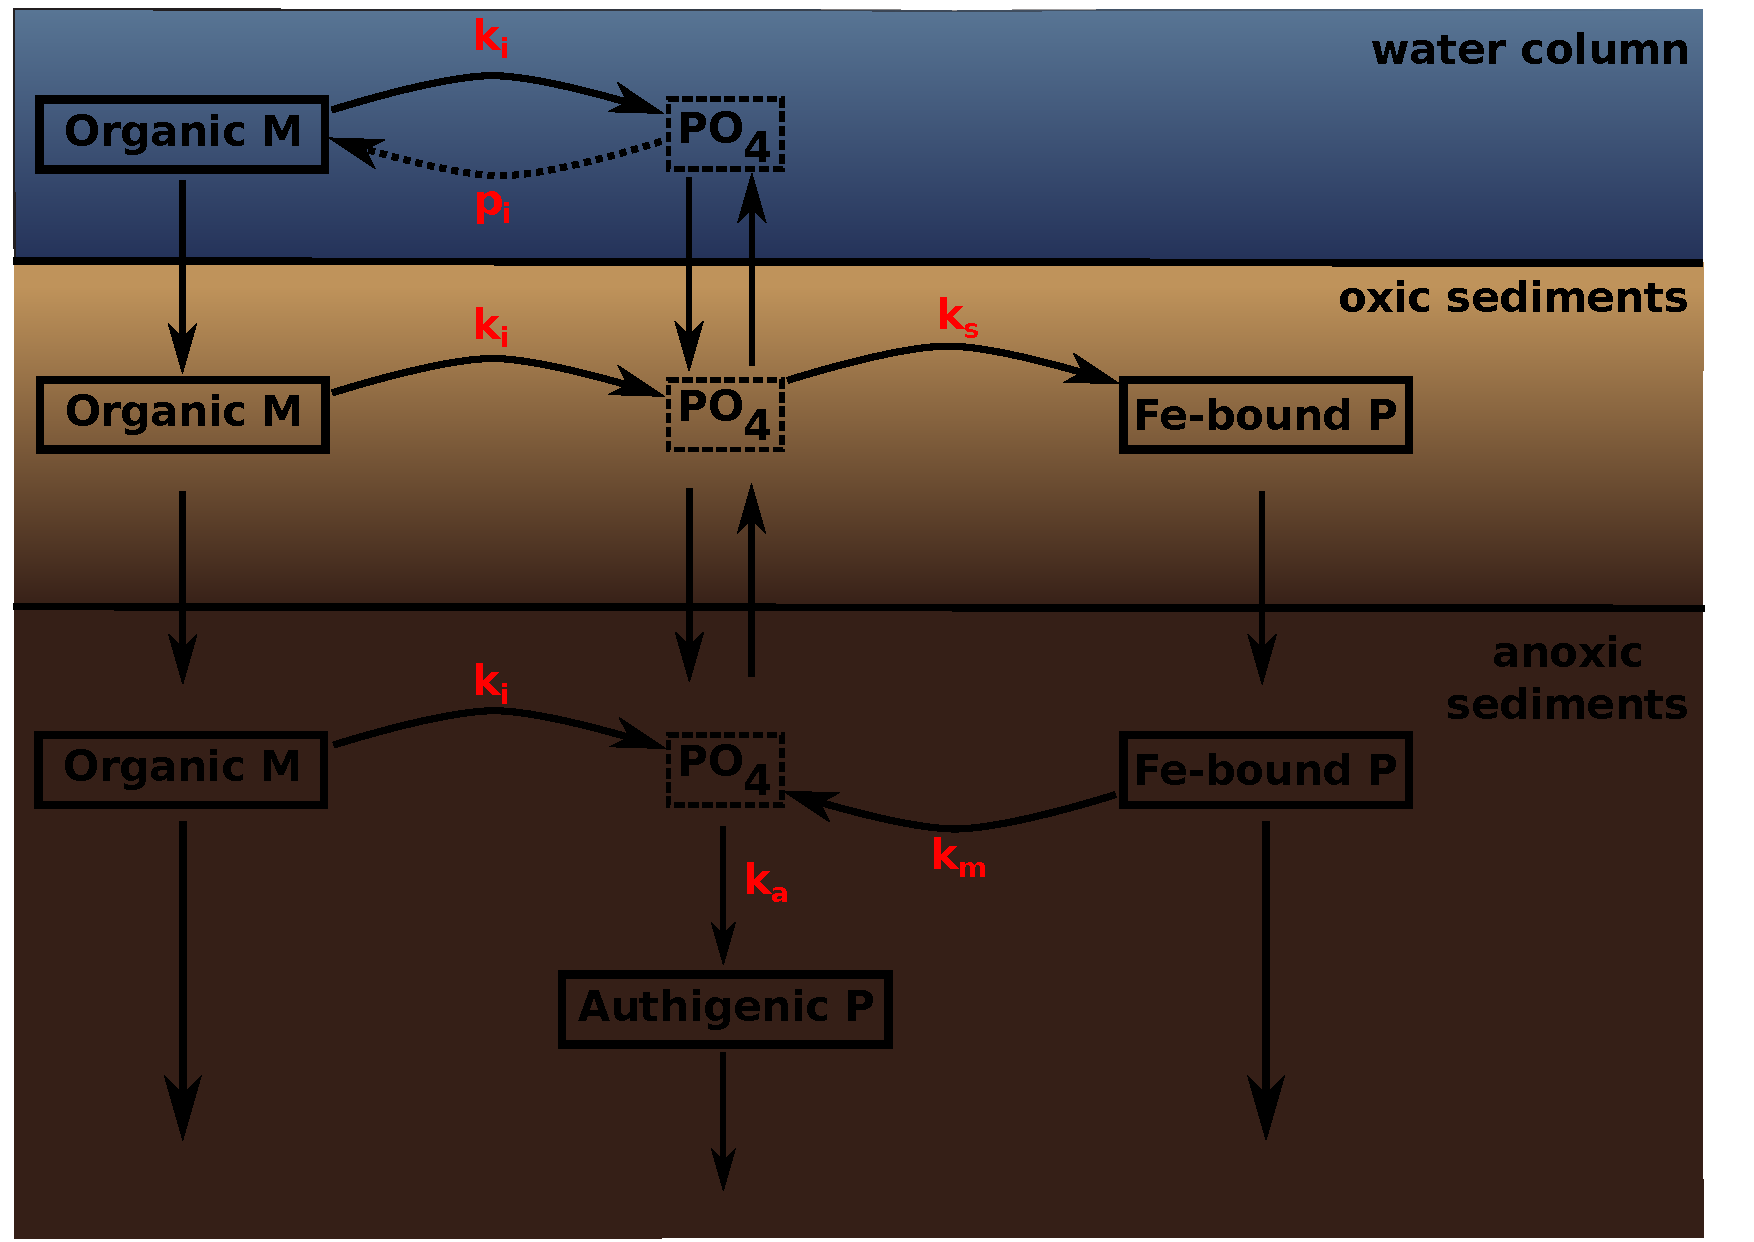
\includegraphics[width=0.8\textwidth]{figures/P-cycle.pdf}
	\caption{A schematic of the sedimentary P cycle in OMEN-SED. Red numbers represent kinetic rate constants for phosphorus dynamics (compare Table \ref{table:reaction_parameters}; p$_i$ represents uptake rate of PO$_4$ 
	via primary production in shallow environments). Adapted from \citet{caroline_p_slomp_key_1996}.}
	\label{fig:P-cycle}
	\end{center}
\end{figure}

The biogeochemical description of phosphorus (P) dynamics builds on the work of \citet{caroline_p_slomp_key_1996} and accounts for phosphorus recycling through organic matter degradation, adsorption onto sediments and 
iron(III) hydroxides (Fe-bound P), as well as carbonate fluorapatite (\chem{CFA} or authigenic P) formation (see Figure \ref{fig:P-cycle} for a schematic overview of the sedimentary P cycle). 
In the oxic zone of the sediment, \chem{PO_4} liberated through organic matter degradation can adsorb 
to iron(III) hydroxides forming Fe-bound P \citep[or \chem{FeP},][]{slomp1998role}. Below the oxic zone,  \chem{PO_4} is not only produced via organic matter degradation but can also be released from the Fe-bound P pool due to the 
reduction of iron(III) hydroxides under anoxic conditions. Furthermore, in these zones phosphate concentrations build up and pore waters can thus become supersaturated with respect to carbonate fluorapatite, 
thus triggering the authigenic formation of \chem{CFA} \citep{cappellen_mathematical_1988}. Phosphorus bound in these authigenic minerals represents a permanent sink for reactive phosphorus \citep{caroline_p_slomp_key_1996}. 
As for ammonium, the adsorption of P to the sediment matrix is treated as an equilibrium processes, parameterised with dimensionless adsorption coefficients for the oxic and anoxic zone, 
respectively \citep[$K_\chem{PO_4}^{\mathrm{ox}}$, $K_\chem{PO_4}^{\mathrm{anox}}$][]{slomp1998role}. 
The sorption and desorption of P to iron(III) hydroxides as well as the authigenic fluorapatite formation are described as first-order reactions with rate constants $k_s$, $k_m$ and $k_a$, respectively (Table \ref{table:reaction_parameters}). 
The rate of the respective process is calculated as the product of the rate constant and the difference between the current concentration (of \chem{PO_4} and \chem{FeP}) and an equilibrium or asymptotic concentration \citet{caroline_p_slomp_key_1996}. 
The asymptotic Fe-bound P concentration is $\chem{FeP}^\infty$ and the equilibrium concentration for P sorption and authigenic fluorapatite formation are $\chem{PO_4}^s$ and $\chem{PO_4}^a$, respectively (Table \ref{table:reaction_parameters}). 
The last term in Eq. (\ref{eq:PO4_ODE_L1}) and (\ref{eq:M_ODE_L1}) represents sorption of \chem{PO_4} to \chem{FeP} in the oxic zone, the last term in 
Eq. (\ref{eq:M_ODE_L2}) and (\ref{eq:PO4_ODE_L2}) is the release of \chem{PO_4} from the \chem{FeP} pool and the 4th term in Eq. (\ref{eq:PO4_ODE_L2}) represents the permanent 
loss of \chem{PO_4} to authigenic fluorapatite formation. 
The conservation equations for phosphate and Fe-bound P are thus given by:
\begin{align}
\intertext{1. Oxic zone ($z \leq z_{\mathrm{ox}}$)}
 \frac{\partial \chem{PO_4}^I}{\partial t} &= \frac{D_{\chem{PO_4}}}{1+K_\chem{PO_4}^{\mathrm{ox}}} \frac{\partial^2\chem{PO_4}^I }{\partial z^2} - w\frac{\partial \chem{PO_4}^I }{\partial z} + \frac{1-\phi}{\phi}\frac{1}{1+K_\chem{PO_4}^{\mathrm{ox}}}\sum_i 
					\left( \chem{PC}_i \cdot k_i \cdot \chem{POC}_{i}(z) \right) \notag\\
					& - \frac{k_{s}}{1+K_\chem{PO_4}^{\mathrm{ox}}}(\chem{PO_4}^I-\chem{PO_4}^s)\label{eq:PO4_ODE_L1}\\  %&\text{1. Layer ($z\leq z_{\mathrm{\mathrm{ox}}} \leq zbio$)}\label{eq:SO4_ODE1_Case1_sub1}\\
 \frac{\partial \chem{FeP}^I}{\partial t} &= D_{\chem{FeP}}\frac{\partial^2\chem{FeP}^I }{\partial z^2} - w\frac{\partial \chem{FeP}^I }{\partial z} + \frac{\phi}{1-\phi}k_{s}(\chem{PO_4}^I-\chem{PO_4}^s)\label{eq:M_ODE_L1}\\  
 \intertext{2. Anoxic zones ($z_{\mathrm{ox}} < z \leq z_{\infty}$)} 
 \frac{\partial \chem{FeP}^{II}}{\partial t} & = D_{\chem{FeP}}\frac{\partial^2\chem{FeP}^{II} }{\partial z^2} - w\frac{\partial \chem{FeP}^{II} }{\partial z} - k_{m}(\chem{FeP}^{II} - \chem{FeP}^\infty)\label{eq:M_ODE_L2}\\  
 \frac{\partial \chem{PO_4}^{II}}{\partial t} &= \frac{D_{\chem{PO_4}}}{1+K_\chem{PO_4}^{\mathrm{anox}}} \frac{\partial^2\chem{PO_4}^{II} }{\partial z^2} - w\frac{\partial \chem{PO_4}^{II} }{\partial z} + \frac{1-\phi}{\phi} \frac{1}{1+K_\chem{PO_4}^{\mathrm{anox}}}\sum_i 
					\left( \chem{PC}_i \cdot k_i \cdot \chem{POC}_{i}(z) \right) \notag\\
					& - \frac{k_{a}}{1+K_\chem{PO_4}^{\mathrm{anox}}}(\chem{PO_4}^{II}-\chem{PO_4}^a) + \frac{(1-\phi)}{\phi}\frac{k_{m}}{1+K_\chem{PO_4}^{\mathrm{anox}}}(\chem{FeP}^{II}-\chem{FeP}^\infty)\label{eq:PO4_ODE_L2}
\end{align}
% where
% \begin{align}
%  D_{\chem{PO_4}}&=D_{\chem{PO_4}, 0}+D_{\mathrm{bio}} &\text{ and }\quad D_{\chem{FeP}}&= D_{\mathrm{bio}} &\text{if ($z\leq z_{\mathrm{bio}}$)}\\
%  D_{\chem{PO_4}}&=D_{\chem{PO_4}, 0} &\text{ and }\quad D_{\chem{FeP}}&= 0 &\text{if ($z > z_{\mathrm{bio}}$)} 
% \end{align}
where $D_\chem{PO_4}$ denotes the diffusion coefficient for \chem{PO_4} which depends on the bioturbation status of the respective geochemical zone and 
$D_{\chem{FeP}}=D_{\mathrm{bio}}$ for $z\leq z_{\mathrm{bio}}$ and $D_{\chem{FeP}}=0$ for $z > z_{\mathrm{bio}}$ (compare Section \ref{subsec:GBCM}). 
Integration of Eq. (\ref{eq:PO4_ODE_L1}) - (\ref{eq:PO4_ODE_L2}) yields the analytical solution and Table \ref{Tab:BC_PO4+M} summarises the boundary conditions applied in OMEN-SED.
The model assumes known bottom water concentrations and equal concentrations and diffusive fluxes at $z_{\mathrm{bio}}$ and $z_{\mathrm{ox}}$ for both species. 
Additionally OMEN-SED considers no change in phosphate flux and an asymptotic Fe-bound P concentration at $z_\infty$.
%A no flux boundary condition is applied at $z_\infty$.
%>>>
\marginnote{\textbf{DH}: I think what I wrote before also applies: a asymptotic Fe-bound P concentration at $z_{\infty}$ is assumed! (but is the same as ``no flux condition'' as it is now?')}[-2cm]%<<<
%>>>



\begin{table}[tbp]
\caption{Boundary conditions for phosphate and Fe-bound P (\chem{FeP}). For the boundaries we define:  $z^-_{\_\_} := \lim_{h\to0} (z_{\_\_}-h)$ and $z^+_{\_\_} := \lim_{h\to0} (z_{\_\_}+h)$.}
% title of Table
\centering
% used for centering table
\begin{tabular}{ |l| l| l|}
\hline
\textbf{Boundary}& \textbf{Condition}&\\
\hline
$z=0$& known concentration& 1) \chem{PO_4}(0)=\chem{PO_{40}}  \\
$z=z_{\mathrm{bio}}$&continuity& 2) $\chem{PO_4}(z_{\mathrm{bio}}^-)$=$\chem{PO_4}(z_{\mathrm{bio}}^+)$\\
               & flux & 3) $\left(D_{\chem{PO_4},0}+D_{\mathrm{bio}}\right )\cdot \frac{\partial \chem{PO_4}}{\partial z}|_{z_{\mathrm{bio}}^-}=D_{\chem{PO_4},0} \cdot \frac{\partial \chem{PO_4}}{\partial z}|_{z_{\mathrm{bio}}^+}$\\
$z=z_{\mathrm{ox}}$& continuity& 4) $\chem{PO_4}(z_{\mathrm{ox}}^-)$=$\chem{PO_4}(z_{\mathrm{ox}}^+)$\\
               & flux & 5) $-\frac{D_{\chem{PO_4}}}{1+K_\chem{PO_4}^{ox}} \cdot \frac{\partial \chem{PO_4}}{\partial z}|_{z_{\mathrm{ox}}^-} =-\frac{D_{\chem{PO_4}}}{1+K_\chem{PO_4}^{\mathrm{anox}}} \cdot \frac{\partial \chem{PO_4}}{\partial z}|_{z_{\mathrm{ox}}^+}$\\
%&where:\textcolor{red}{$\int_{z_{\chem{SO_4}}}^{\infty}$ here?} & $\quad F_{\chem{H_2S}}(z_{\mathrm{ox}})=\frac{1-\phi}{\phi} \cdot \textcolor{red}{\gamma_{\chem{H_2S}}\cdot} \left( \int_{z_{\chem{NO_3}}}^{SO_4}  \sum_i SO_4C \cdot k_i \cdot \chem{POC}_i\ dz + \gamma_{CH_4}\cdot \int_{z_{\chem{SO_4}}}^{\infty}  \sum_i SO_4C \cdot k_i \cdot \chem{POC}_i\ dz \right)$\\          
$z=z_{\infty}$& flux & 10) $\frac{\partial \chem{PO_4}}{\partial z}|_{z_\infty}=0$\\
\hline
$z=0$& known concentration& 1) $\chem{FeP}(0)=\chem{FeP}_0$  \\
$z=z_{\mathrm{bio}}$&continuity& 2) $\chem{FeP}(z_{\mathrm{bio}}^-)$=$\chem{FeP}(z_{\mathrm{bio}}^+)$\\
  & flux & 3) $\frac{\partial \chem{FeP}}{\partial z}|_{z_{\mathrm{bio}}^-}=\frac{\partial \chem{FeP}}{\partial z}|_{z_{\mathrm{bio}}^+}$\\
$z=z_{\mathrm{ox}}$& continuity& 4) $\chem{FeP}(z_{\mathrm{ox}}^-)$=$\chem{FeP}(z_{\mathrm{ox}}^+)$\\
  & flux & 5) $\frac{\partial \chem{FeP}}{\partial z}|_{z_{\mathrm{ox}}^-} =\frac{\partial \chem{FeP}}{\partial z}|_{z_{\mathrm{ox}}^+}$\\
%&where:\textcolor{red}{$\int_{z_{\chem{SO_4}}}^{\infty}$ here?} & $\quad F_{\chem{H_2S}}(z_{\mathrm{ox}})=\frac{1-\phi}{\phi} \cdot \textcolor{red}{\gamma_{\chem{H_2S}}\cdot} \left( \int_{z_{\chem{NO_3}}}^{SO_4}  \sum_i SO_4C \cdot k_i \cdot \chem{POC}_i\ dz + \gamma_{CH_4}\cdot \int_{z_{\chem{SO_4}}}^{\infty}  \sum_i SO_4C \cdot k_i \cdot \chem{POC}_i\ dz \right)$\\          
$z=z_{\infty}$& asymptotic concentration & 10) $\chem{FeP}(z_\infty)=\chem{FeP}_\infty$\\
\hline    
\end{tabular}
\label{Tab:BC_PO4+M}
% is used to refer this table in the text
\end{table}


\subsubsection{Dissolved Inorganic Carbon (DIC)}\label{subsubsec:DIC}
OMEN-SED accounts for the production of dissolved inorganic carbon (\chem{DIC}) through organic matter degradation, as well as methane oxidation. 
Organic matter degradation produces dissolved inorganic carbon with a stoichiometric \chem{DIC:C} ratio of 1:2 in the methanic zone and 1:1 in the rest of the sediment column (\chem{DICC^{II}} and \chem{DICC^{I}} respectively). 
\chem{DIC} production through methane oxidation is implicitly taken into account through the boundary condition at $z_{\chem{SO_4}}$. 
A mechanistic description of \chem{DIC} production from \chem{CaCO_3} dissolution %is in coastal marine significantly smaller than its production from OM degradation \citep{krumins_dissolved_2013} and 
would lead to significant mathematical problems and is therefore not included in the current version of OMEN-SED. 
The conservation equations for \chem{DIC} are thus given by:
\begin{align}
\intertext{1. Oxic, nitrogenous and sulfidic zone ($z \leq z_{\chem{SO_4}}$)}
  \frac{\partial \chem{DIC}^I}{\partial t} &= 0 = D_{\chem{DIC}} \frac{\partial^2\chem{DIC}^I }{\partial z^2} - w\frac{\partial \chem{DIC}^I }{\partial z} + \frac{1-\phi}{\phi} \cdot \sum_i \chem{\chem{DIC}C^I} \cdot k_i \cdot \chem{POC}_{i}(z)\label{eq:DIC_ODE1_L1}\\ %\qquad &\text{1. Layer ($z\leq z_{\mathrm{ox}}$)}\\
 \intertext{2. Methanic zone ($z_{\chem{SO_4}} < z \leq z_\infty$)} 
  \frac{\partial \chem{DIC}^{II}}{\partial t} &= 0 = D_{\chem{DIC}} \frac{\partial^2\chem{DIC}^{II} }{\partial z^2} - w\frac{\partial \chem{DIC}^{II} }{\partial z} + \frac{1-\phi}{\phi} \cdot \sum_i \chem{\chem{DIC}C^{II}} \cdot k_i \cdot \chem{POC}_{i}(z)\label{eq:DIC_ODE1_L2} %\qquad &\text{1. Layer ($z\leq z_{\mathrm{ox}}$)}\\
\end{align}
where $D_\chem{\chem{DIC}}$ denotes the diffusion coefficient for \chem{DIC} which depends on the bioturbation status of the respective geochemical zone. 
Integration of Eq. (\ref{eq:DIC_ODE1_L1}) and (\ref{eq:DIC_ODE1_L2}) yields the analytical solution and Table \ref{Tab:BC_DIC} summarises the boundary conditions applied in OMEN-SED. 
A Dirichlet condition is applied at the sediment-water interface. In addition, the model assumes a zero diffsive flux through the lower boundary $z_\infty$ and continuity across the bottom of the bioturbated zone, as well as the sulfate penetration depth. An additional flux boundary condition at $z_{\chem{SO_4}}$, implicitly accounts for DIC production through anaerobic oxidation of methane  (Table \ref{Tab:BC_DIC} Eq. 5).

\begin{table}[tbp]
\caption{Boundary conditions for \chem{DIC}. For the boundaries we define:  $z^-_{\_\_} := \lim_{h\to0} (z_{\_\_}-h)$ and $z^+_{\_\_} := \lim_{h\to0} (z_{\_\_}+h)$.}
% title of Table
\centering
% used for centering table
\begin{tabular}{ |c| c| c l|}
\hline
\textbf{Boundary}& \textbf{Condition}&&\\
\hline
$z=0$& known concentration& 1)& $\chem{DIC}(0)=\chem{DIC}_{0}$  \\
$z=z_{\mathrm{bio}}$&continuity& 2)& $\chem{DIC}(z_{\mathrm{bio}}^-)$=$\chem{DIC}(z_{\mathrm{bio}}^+)$\\
               & flux & 3)& $-\left(D_{\chem{DIC},0}+D_{\mathrm{bio}}\right )\cdot \frac{\partial \chem{DIC}}{\partial z}|_{z_{\mathrm{bio}}^-}=-D_{\chem{DIC},0} \cdot \frac{\partial \chem{DIC}}{\partial z}|_{z_{\mathrm{bio}}^+}$\\
$z=z_{\chem{SO_4}}$& continuity & 4)& $\chem{DIC}(z_{\chem{SO_4}}^-)$=$\chem{DIC}(z_{\chem{SO_4}}^+)$\\ %$\frac{\partial \chem{DIC}}{\partial z}|_{z_{\chem{DIC}}}=0$\\
               & flux (with AOM) & 5)&  $-D_{\chem{DIC}}\cdot \frac{\partial \chem{DIC}}{\partial z}|_{z_{\chem{SO_4}}^-} + \gamma_\chem{CH_4}\cdot F_{\chem{CH_4}}(z_{\chem{SO_4}})=-D_{\chem{DIC}} \cdot \frac{\partial \chem{DIC}}{\partial z}|_{z_{\chem{SO_4}}^+}$\\
&where: & &$\quad F_{\chem{CH_4}}(z_{\chem{SO_4}})=\frac{1-\phi}{\phi} \cdot \int_{z_{\chem{SO_4}}}^{\infty}  \sum_i \chem{MC} \cdot k_i \cdot \chem{POC}_i\ dz$ \\          
$z=z_{\infty}$& zero \chem{DIC} flux & 6)& $\frac{\partial \chem{DIC}}{\partial z}|_{z_\infty}=0$\\
\hline
\end{tabular}
\label{Tab:BC_DIC}
\end{table}


\subsubsection{Alkalinity}\label{subsubsec:ALK}
%>>>
\marginnote{\textbf{SA}: \textbf{TODO: again need to mention carboantes}}[-0cm]%<<<
%>>>
Organic matter degradation and secondary redox reactions exert a complex influence on alkalinity  \citep[e.g.][]{jourabchi_quantitative_2005, wolf-gladrow_total_2007, krumins_dissolved_2013}. 
To model alkalinity, OMEN-SED divides the sediment column is into four geochemical zones, 
where different equations describe the biogeochemical processes using variable stoichiometric coefficients (compare values in Table \ref{table:reaction_parameters}). 
Above $z_{\mathrm{ox}}$, the combined effects of \chem{NH_4} and \chem{P} release due to aerobic OM degradation increases alkalinity according to $\chem{ALK}^\mathrm{OX}$ whereas nitrification decreases alkalinity with stoichiometry 
$\chem{ALK}^\mathrm{NIT}$. 
In the remaining three zones anaerobic OM degradation generally results in an increase in alkalinity, with the exact magnitude depending on the nature of the terminal electron acceptor used 
(i.e. $\chem{ALK}^\mathrm{DEN}$, $\chem{ALK}^\mathrm{SUL}$, $\chem{ALK}^\mathrm{MET}$). In addition, the effect of secondary redox reactions, such as nitrification, sulfide and methane oxidation are implicitly accounted for in the boundary conditions. 
Again, a mechanistic description of \chem{ALK} production from \chem{CaCO_3} dissolution %is in coastal marine sediments the second largest source of ALK after OM degradation via sulfate reduction \citep{krumins_dissolved_2013} 
would lead to significant mathematical problems and is therefore not included in the current version of OMEN-SED. 
In OMEN-SED, the conservation equations for alkalinity are thus given by:
\begin{align}
 \intertext{1. Oxic zone ($z \leq z_{\chem{ox}}$)} 
\frac{\partial \chem{ALK}^{I}}{\partial t} &= 0 = D_{\chem{ALK}} \frac{\partial^2\chem{ALK}^{I} }{\partial z^2} - w\frac{\partial \chem{ALK}^{I} }{\partial z} \notag\\
					  & + \frac{1-\phi}{\phi} \cdot \sum_i \left( \chem{ALK}^\mathrm{NIT} \cdot \frac{\gamma_{\chem{NH_4}}}{1+K_\chem{NH_4}} \chem{NC_i} + \chem{ALK}^\mathrm{OX}\right)\cdot k_i \cdot \chem{POC}_{i}(z) \label{eq:ALK_ODE1_L1}\\
 \intertext{2. Dentrification or nitrogenous zone ($z_{\chem{ox}} < z \leq z_{\chem{NO_3}} $)} 
\frac{\partial \chem{ALK}^{II}}{\partial t} &= 0 = D_{\chem{ALK}} \frac{\partial^2\chem{ALK}^{II} }{\partial z^2} - w\frac{\partial \chem{ALK}^{II} }{\partial z} + \frac{1-\phi}{\phi} \cdot \sum_i \chem{ALK}^\mathrm{DEN}\cdot k_i \cdot \chem{POC}_{i}(z)\label{eq:ALK_ODE1_L2}
 \intertext{3. Sulfidic zone ($z_{\chem{NO_3}} < z \leq z_{\chem{SO_4}} $)} 
\frac{\partial \chem{ALK}^{III}}{\partial t} &= 0 = D_{\chem{ALK}} \frac{\partial^2\chem{ALK}^{III} }{\partial z^2} - w\frac{\partial \chem{ALK}^{III} }{\partial z} + \frac{1-\phi}{\phi} \cdot \sum_i \chem{ALK}^\mathrm{SUL}\cdot k_i \cdot \chem{POC}_{i}(z)\label{eq:ALK_ODE1_L3}
 \intertext{4. Methanic zone ($z_{\chem{SO_4}} < z \leq z_{\infty} $)} 
\frac{\partial \chem{ALK}^{IV}}{\partial t} &= 0 = D_{\chem{ALK}} \frac{\partial^2\chem{ALK}^{IV} }{\partial z^2} - w\frac{\partial \chem{ALK}^{IV} }{\partial z} + \frac{1-\phi}{\phi} \cdot \sum_i \chem{ALK}^\mathrm{MET}\cdot k_i \cdot \chem{POC}_{i}(z)\label{eq:ALK_ODE1_L4}
\end{align}
where $D_\chem{\chem{ALK}}$ denotes the diffusion coefficient for alkalinity which depends on the bioturbation status of the respective geochemical zone. 
Integration of Eq. (\ref{eq:ALK_ODE1_L1}) - (\ref{eq:ALK_ODE1_L4}) yields the analytical solution and Table \ref{Tab:BC_ALK} summarises the boundary conditions applied in OMEN-SED. 
A Dirichlet boundary condition is applied at the sediment-water interface. The decrease of alkalinity due to oxidation of reduced species produced in the anoxic zones 
(with stoichiometry $\chem{ALK}^\mathrm{NIT}$ and $\chem{ALK}^\mathrm{H_2S}$) is implicitly taken into account through the flux boundary condition at $z_{\mathrm{ox}}$ (Table \ref{Tab:BC_ALK} Eq. 5). 
Furthermore, the oxidation of methane by sulfate reduction increases alkalinity with stoichiometry $\chem{ALK}^\mathrm{AOM}$ which is accounted for through the flux boundary condition at $z_{\chem{SO_4}}$ (Table \ref{Tab:BC_ALK} Eq. 9). 
At the lower boundary $z_\infty$ a zero diffusive flux condition is applied. 

\begin{table}[tbp]
\caption{Boundary conditions for alkalinity. For the boundaries we define:  $z^-_{\_\_} := \lim_{h\to0} (z_{\_\_}-h)$ and $z^+_{\_\_} := \lim_{h\to0} (z_{\_\_}+h)$.}
% title of Table
\centering
% used for centering table
\begin{tabular}{ |c| c| c l|}
\hline
\textbf{Boundary}& \textbf{Condition}&&\\
\hline
$z=0$& known concentration& 1)& $\chem{ALK}(0)=\chem{ALK}_{0}$  \\
$z=z_{\mathrm{bio}}$&continuity& 2)& $\chem{ALK}(z_{\mathrm{bio}}^-)$=$\chem{ALK}(z_{\mathrm{bio}}^+)$\\
               & flux & 3)& $-\left(D_{\chem{ALK},0}+D_{\mathrm{bio}}\right )\cdot \frac{\partial \chem{ALK}}{\partial z}|_{z_{\mathrm{bio}}^-}=-D_{\chem{ALK},0} \cdot \frac{\partial \chem{ALK}}{\partial z}|_{z_{\mathrm{bio}}^+}$\\
$z=z_{\mathrm{ox}}$& continuity& 4)& $\chem{ALK}(z_{\mathrm{ox}}^-)$=$\chem{ALK}(z_{\mathrm{ox}}^+)$\\
               & flux & 5)& $-D_{\chem{ALK}} \cdot \frac{\partial \chem{ALK}}{\partial z}|_{z_{\mathrm{ox}}^-} +  F_{\chem{ALK}}(z_{\mathrm{ox}})=-D_{\chem{ALK}} \cdot \frac{\partial \chem{ALK}}{\partial z}|_{z_{\mathrm{ox}}^+}$\\
&where: & &$\quad F_{\chem{ALK}}(z_{\mathrm{ox}})=\frac{1-\phi}{\phi} \cdot \left( \chem{ALK}^\chem{H_2S}\cdot \gamma_\chem{H_2S} \int_{z_{\chem{NO_3}}}^{\chem{SO_4}} \sum_i \chem{SO_4C} \cdot k_i \cdot \chem{POC}_i\ dz \right)$\\
& & &$\qquad \qquad \qquad \quad + \frac{1-\phi}{\phi} \cdot \left(\chem{ALK}^\chem{NIT} \frac{\gamma_\chem{NH_4}}{1+k_\chem{NH_4}}\int_{z_{\chem{NO_3}}}^{\infty}  \sum_i \chem{NC_i} \cdot k_i \cdot \chem{POC}_i\ dz \right)$\\            
$z=z_{\chem{NO_3}}$&continuity& 6)& $\chem{ALK}(z_{\chem{NO_3}}^-)$=$\chem{ALK}(z_{\chem{NO_3}}^+)$\\
               & flux & 7)& $-D_{\chem{ALK}}\cdot \frac{\partial \chem{ALK}}{\partial z}|_{z_{\chem{NO_3}}^-}=-D_{\chem{ALK}} \cdot \frac{\partial \chem{ALK}}{\partial z}|_{z_{\chem{NO_3}}^+}$\\
$z=z_{\chem{SO_4}}$& continuity & 8)& $\chem{ALK}(z_{\chem{SO_4}}^-)$=$\chem{ALK}(z_{\chem{SO_4}}^+)$\\ %$\frac{\partial \chem{ALK}}{\partial z}|_{z_{\chem{ALK}}}=0$\\
               & flux (with AOM) & 9)&  $-D_{\chem{ALK}}\cdot \frac{\partial \chem{ALK}}{\partial z}|_{z_{\chem{SO_4}}^-} + F_{\chem{ALK}}(z_{\chem{SO_4}})=-D_{\chem{ALK}} \cdot \frac{\partial \chem{ALK}}{\partial z}|_{z_{\chem{SO_4}}^+}$\\
&where: & &$\quad F_{\chem{ALK}}(z_{\chem{SO_4}})=\frac{1-\phi}{\phi} \cdot \left( \chem{ALK}^\chem{AOM}\gamma_\chem{CH_4}\cdot \int_{z_{\chem{SO_4}}}^{\infty}  \sum_i k_i \cdot \chem{POC}_i\ dz \right)$ \\          
$z=z_{\infty}$& zero \chem{ALK} flux & 10)& $\frac{\partial \chem{ALK}}{\partial z}|_{z_\infty}=0$\\
\hline    
\end{tabular}
\label{Tab:BC_ALK}
\end{table}

\subsection{Determination of Integration Constants}\label{subsec:Determine_IC}

The integration constants of all general analytical solutions derived above change in response to changing boundary conditions. Thus, OMEN-SED has to re-determine integration constants for each dynamic zone 
(i.e. $z_{\mathrm{ox}}, z_{\mathrm{bio}}, z_{\chem{NO_3}}$ and $z_{\chem{SO_4}}$) at every time step for all biogeochemnical tracers. The bioturbation boundary poses a particular challenge as it can theoretically occur in any of the dynamic geochemical 
zones (Fig. \ref{fig:Boundary_matching_algo}). Therefore, in order to generalise and simplify this recurring boundary matching problem, an independent, generic algorithm 
is implemented (rather than using multiple fully-worked-out algebraic solutions for each possible case and every biogeochemical tracer). 
The algorithm only has to solve a two-simultaneous-equation problem.

\subsubsection{Generic Boundary Condition Matching (GBCM)}\label{subsec:GBCM}
% A general steady-state transport-reaction equation for the set of coupled reaction-tansport equations for a generic tracer $C$ implemented in OMEN-SED can be formulated as:
% 
% \begin{align} 
%  \frac{\partial C}{\partial t} &= 0 = D\frac{\partial^2C }{\partial z^2} - w\frac{\partial C }{\partial z} - k\cdot C - \sum_i \alpha_i \exp(-\beta_i z) + Q \label{eq:generalODE}
% \end{align}
% where $t$ is time, $z$ is sediment depth, $D$ is the diffusion coefficient, $w$ is advection rate and $k$ a generic reaction rate constant. 
% The inhomogeneous reaction (production/consumption) of tracer $C$ is described by $g(z) = \alpha_i \exp(-\beta_i z) + Q$, where $Q$ is a zeroth-order (or constant) rate of $C$ reaction, $\alpha_i$ can be interpreted as 
% the relative importance and $1/\beta_i$ as the length scale of reaction $i$ \citep{boudreau1997diagenetic}. 

As discussed in Section \ref{subsec:GeneralModelApproach}, the solution of the general steady-state transport-reaction equation (Eq. (\ref{eq:generalODE})) for a generic 
tracer $C$ is of the general form:
\begin{align}
 C(z) &= A \exp(az) + B  \exp(bz) + \sum_j \frac{\alpha_j}{D \beta_j^2-w\beta_j-k}\cdot \exp(-\beta_j z) + \frac{Q}{k} \label{eq:ODE_general_solution}
\end{align}
% %>>>
% \marginnote{\textbf{DH}: Should it be $D \beta_i^2+w\beta_i-k$ in the denom. - see \citet{boudreau1997diagenetic} Exp 6-13 Eq. 6.121}[-1.5cm]%<<<
% %>>>
and can therefore be expressed as:
\begin{align}
C(z) = A \cdot E(z) + B \cdot F(z) + G(z) 
\end{align}
where $E(z)$, $F (z)$ are the homogeneous solutions of the ODE, G(z) the particular integral (collectively called the basis functions), and A, B are the integration constants that must be determined with the boundary conditions 
(shown in Fig. \ref{fig:Boundary_matching_algo} for the whole sediment column).

Each internal boundary matching problem (i.e. excluding $z=0$ and $z=z_\infty$) involves matching continuity and flux for the two solutions of the respective 
reaction-transport equation above, $C_U(z)$ (= 'upper'), and below, $C_L(z)$ (= 'lower'), the dynamic boundary at $z = z_b$:
\begin{align}
C_U(z) &= A_U \cdot E_U(z) + B_U \cdot F_U(z) + G_U(z) \label{ODE_solution_U}\\
C_L(z) &= A_L \cdot E_L(z) + B_L \cdot F_L(z) + G_L(z) .\label{ODE_solution_L}
\end{align}
OMEN-SED generally applies concentration continuity and flux boundary conditions at its internal, dynamic boundaries: \\
Continuity (where for generality we allow a discontinuity $V_b$) 
\begin{align}
  C_U(z_b) &= C_L(z_b) + V_b	\\
\intertext{Flux}
 D_U C_U'(z_b) + wC_U(z_b) &=  D_LC_L'(z_b) + wC_L(z_b) + F_b
\end{align}
where $w$ is advection, $D$ are the diffusion coefficients and $F_b$ is any flux discontinuity (e.g. resulting from secondary redox reactions).\\[1em]
Considering that the advective flux above and below the boundary is equal (i.e. $wC_U(z_b) = wC_L(z_b)$) and substituting the general ODE solutions (\ref{ODE_solution_U}), (\ref{ODE_solution_L}), 
the boundary conditions can be represented as two equations connecting the four integration constants:
\begin{equation}
 \begin{pmatrix} E_U & F_U \\ D_UE_U' & D_UF_U' \end{pmatrix} \begin{pmatrix} A_U \\ B_U \end{pmatrix} = \begin{pmatrix} E_L & F_L \\ D_LE_L' & D_LF_L' \end{pmatrix} \begin{pmatrix} A_L \\ B_L \end{pmatrix} 
 + \begin{pmatrix} G_L - G_U + V_b \\ D_LG_L' - D_UG_U' + F_b - wV_b\end{pmatrix} \label{Solution_BC}
\end{equation}
where the ODE solutions $E,\ F,\ G$ are all evaluated at $z_b$.\\[1em]
Equation (\ref{Solution_BC}) can now be solved to give $A_U$ and $B_U$ as a function of the integration constants from the layer below ($A_L$ and $B_L$), thereby constructing a piecewise solution for both layers, 
with just two integration constants (this is implemented in the function \textsf{\textbf{benthic\_utils.matchsoln}} of OMEN-SED): % $A_L$ and $B_L$. \\[1em]
\begin{equation}
\begin{pmatrix} A_U \\ B_U \end{pmatrix} = \begin{pmatrix} c_1 & c_2 \\ c_3 & c_4 \end{pmatrix} \begin{pmatrix} A_L \\ B_L \end{pmatrix} + \begin{pmatrix} d_1 \\ d_2 \end{pmatrix} . \label{Solution_matchsoln} 
\end{equation}
Using Eq. (\ref{Solution_matchsoln}), $C_U(z)$ in (\ref{ODE_solution_U}) can now be rewritten as a function of $A_L$ and $B_L$ (implemented in  \textsf{\textbf{benthic\_utils.xformsoln}})):
\begin{equation}
 C_U(z) = (c_1 A_L + c_2 B_L + d_1) \cdot E_U(z) + (c_3 A_L + c_4 B_L + d_2) \cdot F_U(z) + G_U(z)  \label{Eq:Sol_Upper_rewritten}
\end{equation}
and hence define the ``transformed'' basis functions $E_U^*(z),\ F_U^*(z),\ G_U^*(z)$ such that:
\begin{equation}
 C_U(z) = A_L \cdot E_U^*(z) + B_L \cdot F_U^*(z) + G_U^*(z) \label{Solution_Upper_transformed_basis_fct}
\end{equation}
where
\begin{align}
 E_U^*(z) &= c_1 E_U(z) + c_3 F_U(z) \notag\\
 F_U^*(z) &= c_2 E_U(z) + c_4 F_U(z) \label{Solution_NEW_EFG}\\
 G_U^*(z) &= G_U(z) + d_1 E_U(z) + d_2 F_U(z) \notag
\end{align}

\begin{figure}[htbp]
\begin{center}
	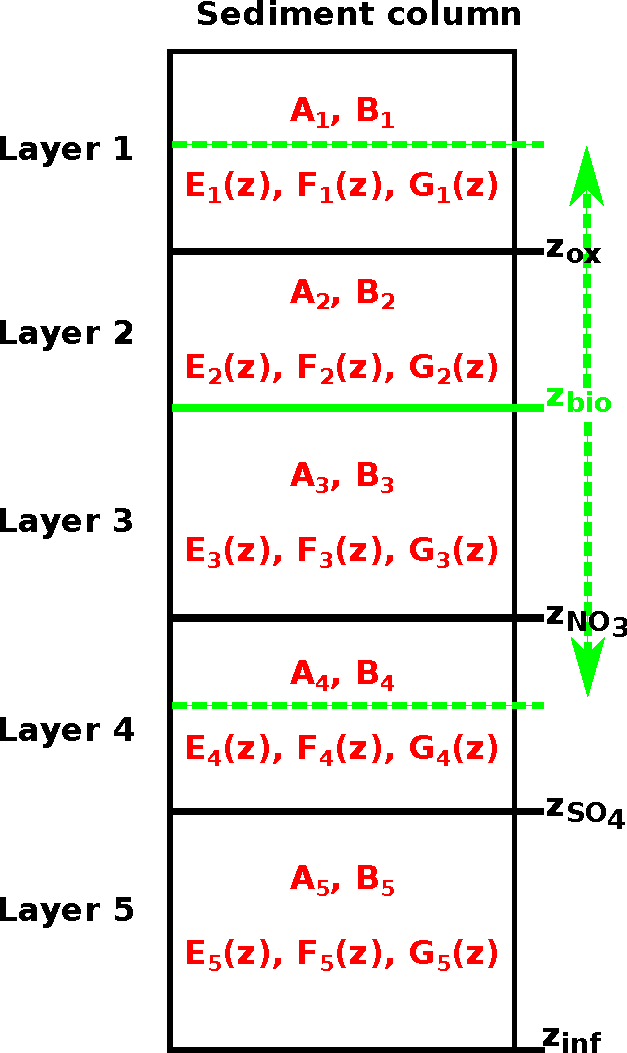
\includegraphics[width=0.3\textwidth]{figures/Boundary_Matching_zbio.pdf}
	\caption{Schematic of the generic boundary condition matching (GBCM) problem. Showing the resulting integration constants ($A_i,\ B_i$) and ODE solutions ($E_i,\ F_i,\ G_i$) for the different sediment layers and the variable 
	bioturbation boundary.}
	\label{fig:Boundary_matching_algo}
	\end{center}
\end{figure}
%\subsubsection*{Application in the model}\label{subsubsec:GBCM-Appl}

Equations (\ref{Solution_matchsoln}), (\ref{Solution_Upper_transformed_basis_fct}) and (\ref{Solution_NEW_EFG}) can now be consecutively applied for each of the dynamic biogeochemical zone boundaries, starting at the bottom of the 
sediment column. The net result is a piecewise solution of the whole sediment column with just two integration constants (coming from the lowest layer), which can then be solved for by applying the boundary conditions at the 
sediment-water interface and the bottom of the sediments. 

\subsubsection{Abstracting out the bioturbation boundary}
The bioturbation boundary affects the diffusion coefficient of the modelled solutes, as well as the conservation equation of organic matter (and thereby the exact form of each reaction-transport equation). 
This boundary is particularly inconvenient as it can, in principle, occur in the middle of any of the dynamically shifting biogeochemical zones and therefore generate multiple cases 
(Fig. \ref{fig:Boundary_matching_algo}). 
The GBCM algorithm described above is thus not only used to construct a piecewise solution of the whole sediment column, but also to abstract out the bioturbation boundary. 
For each biogeochemical zone the "bioturbation-status'' is initially tested (i.e. fully bioturbated, fully non-bioturbated, or crossing the bioturbation boundary). 
Therefore, the upper and lower boundaries for the different zones (e.g. for the nitrogenous zone: $z_U = z\mathrm{ox}$, $z_L = z_\chem{NO_3}$), as well as the respective reactive terms and diffusion coefficients 
(bioturbated and non-bioturbated) are passed over to the routine \textsf{\textbf{zTOC.prepfg\_l12}} where the bioturbation-status is determined. In case the bioturbation depth is located within this zone 
(i.e. $z_U < z_\mathrm{bio} < z_L$) a piecewise solution for this layer is constructed. Therefore, the reactive terms and diffusion coefficients are handed over to the routines \textsf{\textbf{zTOC.calcfg\_l1}} and 
\textsf{\textbf{zTOC.calcfg\_l2}} which calculate the basis functions ($E_U, F_U, G_U$ and  $E_L, F_L, G_L$) and their derivatives for the bioturbated and the non-bioturbated part of this specific geochemical zone. 
The concentration and flux for both solutions at $z_\mathrm{bio}$ are matched and the coefficients $c_1, c_2, c_3, c_4, d_1, d_2$ (as in Eq. (\ref{Solution_matchsoln})) are calculated by the routine 
\textsf{\textbf{benthic\_utils.matchsoln}}. These coefficients and the "bioturbation-status'' of the layer are passed back to the main GBCM algorithm where they can be used by the routine \textsf{\textbf{benthic\_utils.xformsoln}} 
to calculate the ``transformed'' basis functions ($E_U^*(z),\ F_U^*(z),\ G_U^*(z)$) such that both layers are expressed in the same basis (compare Eq. (\ref{Eq:Sol_Upper_rewritten} - \ref{Solution_NEW_EFG}). 
% These new basis functions are now used in the main GBCM algorithm, which therefore never needs to know whether it is dealing with a piecewise solution (i.e. matched across a bioturbation boundary) or a ``simple'' 
% solution (i.e. the layer is fully bioturbated or fully non-bioturbated). 

For instance, in the case of sulfate, \textsf{\textbf{zTOC.prepfg\_l12}} is called three times before the actual profile is calculated (once per zone: oxic, nitrogenous, sulfidic) 
and hands back the information about the ``bioturbation-status'' of the three layers and the coefficients $c_1, c_2, c_3, c_4, d_1, d_2$ for the biogeochemical zone including the bioturbation depth. 
When calculating the complete piecewise solution for the sediment column, this information is passed to the function \textsf{\textbf{zTOC.calcfg\_l12}} which sorts out the correct solution type to use. 
The main GBCM algorithm therefore never needs to know whether 
it is dealing with a piecewise solution (i.e. matched across the bioturbation boundary) or a ``simple'' solution (i.e. the layer is fully bioturbated or fully non-bioturbated). 


\subsection{Model Parameters}\label{subsec:ModelParameters}
The following section provides a summary of  global relationships used to constrain reaction and transport parameters in OMEN-SED. Table \ref{table:sed-charac_transport-parameters} 
synthesises sediment and transport parameters, while table \ref{table:reaction_parameters} provides an overview of all biogeochemical parameters used in OMEN-SED.

\subsubsection{Transport Parameters}
The burial of sediments and pore water is directly related to the accumulation of new material on the seafloor \citep[i.e. sedimentation,][]{burdige2006geochemistry}. 
This results in a downward advective flux of older sediment material and pore water in relation to the sediment-water interface. When coupled to an ocean model, its sedimentation flux can be readily used in OMEN-SED. 
The stand-alone version of OMEN-SED uses the empirical global relationship between sediment accumulation rate (cm yr$^{-1}$) and seafloor depth (m) of \citet{middelburg_empirical_1997}: 
\begin{equation}
 w = 3.3\cdot 10^{-0.87478367-0.00043512\cdot \text{depth}}\label{eq:sedimentation_rate},
\end{equation}
As mentioned before (Section \ref{subsec:GeneralModelApproach}), the diffusion coefficient of species $i$ is calculated as $D_i=D_{i,0}+D_{\mathrm{bio}}=D_{\mathrm{mol},i}\cdot f_{ir}+D_{\mathrm{bio}}$ for dissolved species and $D_i=D_{\mathrm{bio}}$ for solid species. 
The bioturbation coefficient $D_{\mathrm{bio}}$ (cm$^2$ yr$^-1$) is constant in the bioturbated zone and also follows the empirical relationship by \citet{middelburg_empirical_1997}:
\begin{equation}
 D_{\mathrm{bio}} = 5.2\cdot 10^{0.76241122-0.00039724\cdot \text{depth}}\label{eq:bioturbation_coeff}
\end{equation}
Observations indicate that bioturbation is largely restricted to the upper 10 cm of the sediments and is only marginally related to seafloor depth \citep[e.g.][]{boudreau_mean_1998, teal_global_2010}. 
Therefore, OMEN-SED imposes a globally invariant bioturbation depth $z_{\mathrm{bio}}$ of 10 cm. In case the bottom water oxygen concentration is below 5 nmol cm$^{-3}$ 
infaunnal activity is assumed to cease and $z_{\mathrm{bio}} = 0.01$ cm. We choose a low value unequal to zero in order to simplify the implementation of the model. 
This approach ensures that the sediment column always consists of a bioturbated (even though very small for the low oxygen condition) and a non-bioturbated zone, 
thus the same GBCM algorithm can be used to solve the conservation equations. Furthermore, when OMEN-SED is coupled to an Earth system model 
the same method can be used to convert the POC depositional flux into a SWI concentration (i.e. the flux needs to be converted assuming bioturbation, see Section \ref{subsubsec:Methods_ESM_coupling}). 
%>>>
\marginnote{\textbf{SA}: need to explain why not 0; \textbf{DH}: Decent explanation?}[-1cm]%<<<
%>>>

Bioirrigation (i.e the pumping activity by burrow-dwelling animals) exchanges burrow water with overlying water and may enhance the SWI-flux of solutes \citep{aller_importance_1984, aller1988benthic}. 
Several approaches exist to incorporate this into a 1-D diagenetic model, for instance as a non-local transport/exchange process \citep{boudreau_equivalence_1984, emerson_sediment-water_1984} 
or as an enhancement factor of the molecular diffusion coefficient \citep{devol_benthic_1993, soetaert_model_1996}. In OMEN-SED the latter approach is applied and the 
apparent ``bio-diffusion'' coefficient is calculated as $D_{i,0}=D_{\mathrm{mol},i}\cdot f_{ir}$. 
\citet{soetaert_model_1996} derived an empirical relationship between $f_{ir}$ and seafloor depth ($f_{ir} = \mathrm{Min}\{1; 15.9\cdot \mathrm{depth}^{-0.43}\}$) 
based on observations from \citet{archer_benthic_1992} and \citet{devol_benthic_1993}. As this relationship just varies for depth below $\sim$623 m (with a maximum 
value of 3 at $\sim$50 m) a constant value of $f_{ir}=1$ is used in the default OMEN-SED configuration. 
%However, here we do not consider this effect as it is difficult to constrain on geological timescales and set $f_{ir}$ to a constant value of 1 . 
The specific molecular diffusion coefficients $D_{\mathrm{mol},i}$ are corrected for sediment porosity $\phi$, tortuosity F and are linearly interpolated for an ambient 
temperature $T$ using zero-degree coefficients $D^0_i$ and temperature-dependent diffusion coefficients $D^T_i$ \citep[][]{soetaert_model_1996}:
\begin{equation*}
 D_{\mathrm{mol},i} = (D^0_i + D^T_i \cdot T )\cdot \frac{1}{\phi\cdot F}.
\end{equation*}
Tortuosity can be expressed in terms of porosity as $F = \frac{1}{\phi^m}$ \citep{ullman_diffusion_1982} with the exponent $m$ varying according to the type of sediment (here m=3 is used). 
%\textcolor{red}{in matlab: $\phi^{tort-1}$; but see Gypens et al. (2008) the exponent is a parameter m not tortuosity...??}
Values for $D^T_i$ and $D^0_i$ are summarised in Table \ref{table:sed-charac_transport-parameters} and are adapted from \citet{Li_diffusion_1974}, \citet{schulz_quantification_2006} and \citet{gypens_simple_2008}.

\begin{table}[hbtp]
\caption{Sediment characteristics and transport parameters.}
% title of Table
\centering
% used for centering table
\begin{tabular}{l c c l}
% centered columns (6 columns)
\hline\hline
%inserts double horizontal lines
Parameter & Unit  & Value & Description/Source\\
\hline
$\rho_{\mathrm{sed}}$ & g\,cm$^{-3}$ & 2.6 & Sediment density \\
$w$ & cm\,yr$^{-1}$ &  Fct. of seafloor & Advection/Sediment accumulation rate \\
&& depth or from ESM & \citep{middelburg_empirical_1997}\\
$z_{\mathrm{bio}}$& cm & 10 or 0.01 & Bioturbation depth\\
&&&\citep{boudreau_mean_1998, teal_global_2010}\\
$D_{\mathrm{bio}}$& cm$^2$\,yr$^{-1}$ & Fct. of seafloor & Bioturbation coefficient\\
&& depth &\citep{middelburg_empirical_1997}\\
$\phi$ & - & 0.85 & Porosity\\
F & - &  $\frac{1}{\phi^m}$ & Tortuosity, here m=3\\
f$_{ir}$ & - & 1 & Irrigation factor\\
%dispF & - & $irrF \cdot \phi^{F-1.0}$ & Dispersion factor\\
\multicolumn{4}{l}{\textbf{Diffusion coefficients} \citep{Li_diffusion_1974, schulz_quantification_2006, gypens_simple_2008}}\\
$D_{\chem{O_2}}^0$ & cm$^2$\,yr$^{-1}$ & 348.62 &Molecular diffusion coefficient of oxygen at 0$^\circ$C\\
$D_{\chem{O_2}}^T$ & cm$^2$\,yr$^{-1}$\,${}^{\circ}$C$^{-1}$ & 14.09 &Diffusion coefficient for linear temp. dependence of oxygen\\ % value was 0.0386 (changed by Nicolas 2207)
$D_{\chem{NO_3}}^0$ & cm$^2$\,yr$^{-1}$ & 308.42 &Molecular diffusion coefficient of nitrate at 0$^\circ$C\\
$D_{\chem{NO_3}}^T$ & cm$^2$\,yr$^{-1}$\,${}^{\circ}$C$^{-1}$ & 12.26 &Diffusion coefficient for linear temp. dependence of nitrate\\ % value was 0.0386 (changed by Nicolas 2207)
$D_{\chem{NH_4}}^0$ & cm$^2$\,yr$^{-1}$ & 309.05 &Molecular diffusion coefficient of ammonium at 0$^\circ$C\\
$D_{\chem{NH_4}}^T$ & cm$^2$\,yr$^{-1}$\,${}^{\circ}$C$^{-1}$ & 12.26 &Diffusion coefficient for linear temp. dependence of ammonium\\ % value was 0.0386 (changed by Nicolas 2207)
$D_{\chem{SO_4}}^0$ & cm$^2$\,yr$^{-1}$ & 157.68 &Molecular diffusion coefficient of sulfate at 0$^\circ$C\\
$D_{\chem{SO_4}}^T$ & cm$^2$\,yr$^{-1}$\,${}^{\circ}$C$^{-1}$ & 7.88 &Diffusion coefficient for linear temp. dependence of sulfate\\ % value was 0.0386 (changed by Nicolas 2207)
$D_{\chem{H_2S}}^0$ & cm$^2$\,yr$^{-1}$ & 307.48 & Molecular diffusion coefficient of sulfide at 0$^\circ$C\\
$D_{\chem{H_2S}}^T$ & cm$^2$\,yr$^{-1}$\,${}^{\circ}$C$^{-1}$ & 9.64 & Diffusion coefficient for linear temp. dependence of sulfide\\ % value was 0.0386 (changed by Nicolas 2207)
$D_{\chem{PO_4}}^0$ & cm$^2$\,yr$^{-1}$ & 112.91 &Molecular diffusion coefficient of phosphate at 0$^\circ$C\\
$D_{\chem{PO_4}}^T$ & cm$^2$\,yr$^{-1}$\,${}^{\circ}$C$^{-1}$ & 5.59 &Diffusion coefficient for linear temp. dependence of phosphate\\ % value was 0.0386 (changed by Nicolas 2207)
$D_{\chem{DIC}}^0$ & cm$^2$\,yr$^{-1}$ & 151.69  &Molecular diffusion coefficient of DIC at 0$^\circ$C\\
$D_{\chem{DIC}}^T$ & cm$^2$\,yr$^{-1}$\,${}^{\circ}$C$^{-1}$ & 7.93  &Diffusion coefficient for linear temp. dependence of DIC\\ 
$D_{\chem{ALK}}^0$ & cm$^2$\,yr$^{-1}$ & 151.69  &Molecular diffusion coefficient of ALK at 0$^\circ$C\\
$D_{\chem{ALK}}^T$ & cm$^2$\,yr$^{-1}$\,${}^{\circ}$C$^{-1}$ & 7.93 &Diffusion coefficient for linear temp. dependence of ALK\\ 
\multicolumn{4}{l}{Note: DIC and ALK coefficients are the values of $\chem{HCO_3^{-}}$ from \citet{schulz_quantification_2006}.}\\
%\multicolumn{4}{l}{\citep[as in][]{martin_dissolved_1993}. Alkalinity coefficients are the mean values of \chem{NH_4} and \chem{H_2S}.}\\
\hline\hline
\end{tabular}
\label{table:sed-charac_transport-parameters}
% is used to refer this table in the text
\end{table}


\subsubsection {Stoichiometries and reaction parameters}\label{subsubsec:Stoich_reaction_params}
%The parameters relating to organic matter %The overall reactions implemented in OMEN-SED are listed in Table \ref{table:reactions_processes}. 
The first-order organic matter degradation constants of compound class $i$, $k_i$ (yr$^{-1}$), are assumed invariant along the sediment column and therefore independent of the nature 
of the terminal electron acceptor. The rate constants can be altered manually to fit observed sediment profiles (compare Section \ref{subsec:SedProfiles}) or related to a master variable 
provided by a coupled Earth system model (e.g. sedimentation rate, compare Section \ref{subsec:Parameterising_OM_rate_const}). 
The partitioning of the bulk OM pool into reactivity classes ($f_i$) is also done manually in the stand-alone version or is provided by the ESM. 
Organic matter degradation releases N, P and DIC to the pore water using Redfield molar ratios \citep{redfield1963influence} and consumes TEA with specific stoichiometries (\chem{O_2C}, \chem{NO_3C}, \chem{SO_4C}) as summarised in Table \ref{table:reaction_parameters}. 
Table \ref{table:Reaction_Network} in the appendix provides a list of reactions and their stoichiometries as implemented in OMEN-SED. 
The effect of OM degradation and secondary redox reactions on total alkalinity is also accounted for via reaction specific stoichiometries representing the release of \chem{NH_4}, \chem{H_2S} and P and is based on \citet[][]{jourabchi_quantitative_2005}. 
%Based on \citet{jourabchi_quantitative_2005} we assume that aerobic organic matter degradation increases alkalinity by 1 mole per mole ammonium released and decreases alkalinity by 2 mole per mole P released \citep{}.
The secondary redox parameters (i.e. $\gamma_{\chem{NH_4}}$, $\gamma_{\chem{H_2S}}$, $\gamma_{\chem{CH_4}}$), accounting for the fraction of reduced substances that are reoxidised, would be ideally parameterised for instance in relation to bottom water 
oxygen concentration or oxygen penetration depth ($z_{\mathrm{ox}}$). \citet{gypens_simple_2008} for example expressed $\gamma_{\chem{NH_4}}$ as a function of oxygen penetration depth ($\gamma_{\chem{NH_4}} = 0.243 \cdot \mathrm{ln}(z_{\mathrm{ox}}) + 1.8479$) 
based on a fitting exercises to a numerical model and showed that the fraction varies between 0.2 for $z_{\mathrm{ox}}=0.1$cm and 1.0 for $z_{\mathrm{ox}}>3$cm. 
Due to mathematical constraints for finding an analytical solution to the model equations these fractions take constant values generally representing oxygenated deep sea conditions. 
The instantaneous equilibrium adsorption coefficients of \chem{NH_4} and \chem{PO_4} ($K_{\chem{NH_4}}$, $K_\chem{PO_4}^{\mathrm{ox}}$, $K_\chem{PO_4}^{\mathrm{anox}}$) are based on \citet{wang_multicomponent_1996} and \citet{slomp1998role}, respectively.
The first order rate constants for sorption of \chem{PO_4} to Fe oxides ($k_s$), release of \chem{PO_4} from Fe-bound P due to Fe-oxide reduction ($k_m$) and 
authigenic CFA precipitation ($k_a$), as well as the pore water equilibrium concentrations for P sorption and CFA precipation 
($\chem{PO_4}^s$, $\chem{PO_4}^a$ ) and the asymptotic concentration for Fe-bound P ($\chem{FeP}^\infty$ ) are taken from  \citet{caroline_p_slomp_key_1996}. 
See Table \ref{table:reaction_parameters} for a complete summary of the parameters and their values.

%are constrained on the basis of ??. The pore water equilibrium concentrations for P sorption and CFA precipation 
%($\chem{PO_4}^s$, $\chem{PO_4}^a$ ) and the asymptotic concentration for Fe-bound P ($\chem{FeP}^\infty$ ) are taken from  \citet{palastanga_long_term_2011}. 
%The phosphorus to carbon ratio represents the composition of organic matter and is chosen as ?? based on ??.\\
%See Table \ref{table:reaction_parameters} for a complete summary of the parameters and their values.

% \textcolor{red}{Or bit longer:}\\
% In the sulfidic and methanic zone the 
% reduction of 1 mol organic matter additionally produces 0.5 mol of hydrogen sulfide (\chem{SO_4C}) and 0.5 mol of methane (\chem{MC}) respectively. 
% In the oxic part of the sediments 1 mol of oxygen is needed to mineralize 1 mol of organic matter (\chem{O_2C}). In the nitrate and sulfate reduction zone 1 mol of organic matter is reduced by 
% 0.8906 mol of nitrate (\chem{NO_3C}) and 0.5 mol of sulfate (\chem{SO_4C}) respectively. \\
%\textcolor{red}{Next bit from Gypens:} Reoxidation occurs in a ratio of 1 mol of oxygen per mol of carbon anoxically mineralized. Similarly, 2 mol of oxygen
%are consumed during nitrification of \chem{NH_4} produced in the anoxic zone. As nitrification may be incomplete in the oxic zone, we similarly allow for part of the ammonium flux to escape reoxidation. 
\begin{table}[btp]
\caption{Values for biogeochemical parameters used in OMEN-SED. The variables $x$, $y$ and $z$ denote the atomic ratio of carbon, nitrogen and phosphorus of the degrading 
organic matter (here set to $C:N:P = 106:16:1$).
%\textcolor{red}{Stoichiometric factor for oxygen and sulfate relates to mol of terminal electron acceptor consumed for 1 mol of organic matter mineralized. 
%NC and MC related to mol of reduced species produces per mol organic matter mineralized. correct???}
}
% title of Table
\centering
% used for centering table
\begin{tabular}{l c c l}
% centered columns (6 columns)
\hline\hline
%inserts double horizontal lines
Parameter/Variable & Unit  & Value & Description\\
\hline
\multicolumn{4}{l}{\textbf{Stoichiometric factors and molecular ratios}}\\
\chem{NC_i} & mol/mol & $\frac{y}{x}=\frac{16}{106}$ & Nitrogen to carbon ratio\\
% & & & \textcolor{red}{refractory fraction, was 2 different ones? why?}\\
% \chem{NC_2} & mol/mol & $\frac{y}{x}=\frac{16}{106}$ & nitrogen to carbon ratio\\
% & & & labile fraction\\
\chem{PC_i} & mol/mol & $\frac{z}{x}=\frac{1}{106}$ & Phosphorus to carbon ratio\\
\chem{MC}& mol/mol & 0.5 & Methane to carbon ratio\\
&&&produced during methanogenesis\\
\chem{DICC^I}& mol/mol & 1.0 & DIC to carbon ratio until \chem{z_{SO_4}}\\
\chem{DICC^{II}}& mol/mol & 0.5 &  DIC to carbon ratio below \chem{z_{SO_4}}\\
\chem{O_2C} & mol/mol & $\frac{x+2y}{x}=\frac{138}{106}$ & Oxygen to carbon ratio\\
\chem{NO_3C} & mol/mol & $\frac{4x+3y}{5x}=\frac{94.4}{106}$ & Nitrate to carbon ratio\\
\chem{SO_4C} & mol/mol & $\frac{1}{2}\chem{O_2C} = \frac{138}{212}$ & Sulfate to carbon ratio\\
$\chem{ALK}^\mathrm{OX}$ & mol/mol & $\frac{y-2z}{x}=\frac{14}{106}$ & ALK from aerobic degradation\\
%>>>
\marginnote{\textbf{DH}: $\chem{ALK}^\mathrm{OX}$ \textcolor{red}{correct?}: y=NH4 prod.; -2z=P release  }[-1cm]%<<<

$\chem{ALK}^\mathrm{NIT}$ & mol/mol & $-2$ & ALK from nitrification\\
$\chem{ALK}^\mathrm{DEN}$ & mol/mol & $\frac{4x+3y-10z}{5x}=\frac{92.4}{106}$ & ALK from denitrification\\
$\chem{ALK}^\mathrm{SUL}$ & mol/mol & $\frac{x+y-2z}{x}=\frac{120}{106}$ & ALK from sulfate reduction\\
$\chem{ALK}^\mathrm{MET}$ & mol/mol & $\frac{y-2z}{x}=\frac{14}{106}$ & ALK from methanogenesis\\
$\chem{ALK}^\mathrm{H_2S}$ & mol/mol & $-2$ & ALK from \chem{H_2S} oxidation\\
$\chem{ALK}^\mathrm{AOM}$ & mol/mol & $2$ & ALK from AOM\\
%$DICC^I$ & $mol/mol$ & 1 & DIC to carbon ratio\\
%& & & until $z_{\chem{SO_4}}$\\
%$DICC^{II}$ & $mol/mol$ & 0.5 & DIC to carbon ratio\\
%& & & for methanogenesis\\[0.5ex]
\multicolumn{4}{l}{\textbf{Secondary reaction parameters}}\\
$\gamma_{\chem{NH_4}}$ & - & 0.9 & Fraction of \chem{NH_4} that is nitrified\\
%& & & in oxic zone\\
$\gamma_{\chem{H_2S}}$ & - & 0.95 & Fraction of \chem{H_2S} that is oxidised\\
%& & & in oxic zone\\
$\gamma_{\chem{CH_4}}$ & - & 0.99 & Fraction of \chem{CH_4} that is oxidised\\
%& & & at $z_{\chem{SO_4}}$\\
\multicolumn{4}{l}{\textbf{Adsorption coefficients} \citep[][]{wang_multicomponent_1996, slomp1998role}} \\
$K_{\chem{NH_4}}$ & - & 1.4 & \chem{NH_4} adsorption coefficient\\
%&&& \citep[][]{wang_multicomponent_1996}\\
$K_\chem{PO_4}^{\mathrm{ox}},\quad K_\chem{PO_4}^{\mathrm{anox}}$ & - & 200.0,\quad 2.0 & \chem{PO_4} adsorption coefficient (oxic, anoxic)\\
%&&& \citep[][]{slomp1998role}\\
% $K_\chem{PO_4}^{\mathrm{anox}}$ & - & \textcolor{red}{1.3} & \chem{PO_4} adsorption coefficient (anoxic)\\
% &&& \citep[][]{slomp1998role}\\
\multicolumn{4}{l}{\textbf{P related parameters} \citep{caroline_p_slomp_key_1996}}\\
$k_s$ & yr$^{-1}$ & 94.9 & Rate constant for \chem{PO_4} sorption\\
$k_m$ & yr$^{-1}$ & 0.193 & Rate constant for Fe-bound P release\\
$k_a$ & yr$^{-1}$ & 0.365 & Rate constant for authigenic CFA precipitation\\
$\chem{PO_4}^s$ & mol\,cm$^{-3}$ & $1\cdot 10^{-9}$ & Equilibrium conc. for P sorption\\
%&&&\citep{caroline_p_slomp_key_1996}\\
$\chem{FeP}^\infty$ & mol\,cm$^{-3}$ & $1.99\cdot 10^{-10}$ & Asymptotic concentration for Fe-bound P\\
%&&&\citep{caroline_p_slomp_key_1996}\\
$\chem{PO_4}^a$ & mol\,cm$^{-3}$ &  $3.7\cdot 10^{-9}$ & Equilibrium conc. for authigenic P precipitation\\
%&&&\citep{caroline_p_slomp_key_1996}\\

% $k_i$ & yr$^{-1}$ & --- & OM degradation rate constants\\
% $k_s$ & yr$^{-1}$ & \textcolor{red}{???} & rate constant for P sorption\\
% $k_m$ & yr$^{-1}$ & \textcolor{red}{???} & rate constant for Fe-bound P release\\
% $k_a$ & yr$^{-1}$ & \textcolor{red}{???} & rate constant for authigenic P formation\\
\hline\hline
% inserts double horizontal lines
\end{tabular}
\label{table:reaction_parameters}
\end{table}


\section{Stand-alone sensitivity analysis and case studies}
% To validate the stand-alone version of OMEN-SED an extensive sensitivity analysis for the most important model parameters is performed and 
% resulting sediment-water interface fluxes are compared with a global database (Section \ref{subsec:SA}). 
% In addition, results of the stand-alone model are compared with observed pore water profiles from different ocean depths (Section \ref{subsec:SedProfiles}) and OMEN-SED 
% simulations of TEA-fluxes along a typical ocean transect are compared with observations and results from a complete, numerical diagenetic model (Section \ref{subsec:globalhypsometry}). 

% (Maybe make sure the following is added to the different sections below).
% % An extensive sensitivity analysis for the most important model parameters is performed with the stand-alone model and resulting sediment-water interface fluxes are compared with a global 
% % database (Section \ref{subsec:SA}). 
% % In addition, results of the stand-alone model are compared with observed pore water profiles from different ocean depths (Section \ref{subsec:SedProfiles}) and OMEN-SED simulations of TEA-fluxes along a typical ocean transect 
% % are compared with observations and results from a complete, numerical diagenetic model (Section \ref{}). Furthermore, OMEN-SED iss coupled to the cGENIE Earth system model 
% % and different published parameterisations for the OM degradation rate constants are tested on a global scale (Section \ref{subsec:GENIE-pre-ind}).

\subsection{Sensitivity Analysis}\label{subsec:SA}
\subsubsection{Methodology}
Model parameters implicitly account for processes that are not explicitly resolved. Therefore, model parameters are notoriously difficult to constrain and a source of uncertainty for numerical and analytical models. 
A comprehensive sensitivity analysis (SA) can help quantify this uncertainty and identify the most sensitive parameters. More specifically, sensitivity analysis is used to investigate how the variations in the outputs 
($y_1,\ ...,\ y_N$) of a model can be attributed to variations in the different input parameters \citep[$x_1,\ ...,\ x_M$,][]{pianosi_sensitivity_2016}. 
Different types of sensitivity indices, which quantify the relative influence of parameter $x_i$ on output $y_j$ with a scalar $S_{i,j}$ 
(for $i \in \{1,\ ...,\ M \}$ and $j \in \{1,\ ...,\ N \}$), can be calculated, ranging from simple one-at-a-time methods to statistical evaluations of the output 
distribution \citep[e.g. variance-based or density-based approaches][]{pianosi_sensitivity_2016}. The latter indices 
%are easy to interpret and can be compared across different parameters and/or different model outputs as they generally 
take values between zero and one ($S_{i,j} \in [0, 1]$), where zero indicates a non-influential parameter and a higher value a more influential parameter. 
Here, SA is used mainly to identify which parameters have the largest impact on the different model outputs and therefore require careful calibration. 
% and if there is any factor whose variability has a negligible effects on specific outputs?
%Due to OMEN-SED's computational efficiency we are able to apply one of the approaches requiring higher numbers of model evaluations to compute the sensitivity index.  
As the probability density functions of our model outputs (i.e. the resulting SWI-fluxes) are generally highly-skewed towards extreme organic matter degradation rates (not shown) variance-based sensitivity indices 
may not be a suitable proxy for output uncertainty \citep{pianosi_sensitivity_2016}. 
Hence the novel density-based PAWN method by \citet{pianosi_simple_2015} is employed which considers the entire conditional and unconditional Cumulative Destribution Function (CDF) of the model output
rather than its variance only. The unconditional CDF, $F_y(y)$, of output $y$ is obtained when all uncertain parameters ($x_1,\ ...,\ x_M$) are varied simultaneously, 
and the conditional CDFs, $F_{y|x_i}(y)$, are obtained when all inputs but the $i$-th parameter are varied (i.e. $x_i$ is fixed to a so-called conditioning value). 
The sensitivity index of parameter $i$ is measured by the distance between the two CDFs using the Kolmogorov-Smirnov statistic 
\citep{kolmogorov1933sulla, smirnov1939estimation}, i.e.:
\begin{equation}
 S_i = \max_{x_i} \max_{y} | F_y(y) - F_{y|x_i}(y) |.
\end{equation}
%where $F_y(y)$ is the unconditional CDF of the output $y$ and $F_{y|x_i}(y)$ represents the conditional CDF when the $i$-th parameter is fixed to the conditioning value. 
Since $F_{y|x_i}(y)$ accounts for what happens when the variability due to $x_i$ is removed, the distance between the two CDFs provides a measure of the effects of
$x_i$ on the output $y$. 
Due to the model complexity it is impossible to compute the sensitivity indices analytically. Therefore, they are approximated from a Latin-Hypercube sampling of parameter 
inputs and calculated outputs.
For a brief description of the methodology see Fig. \ref{fig:Sensitivity_Analysis_methodology}. For more details we refer the interested reader to \citet{pianosi_simple_2015}. 

\begin{figure}[htbp]
\begin{center}
	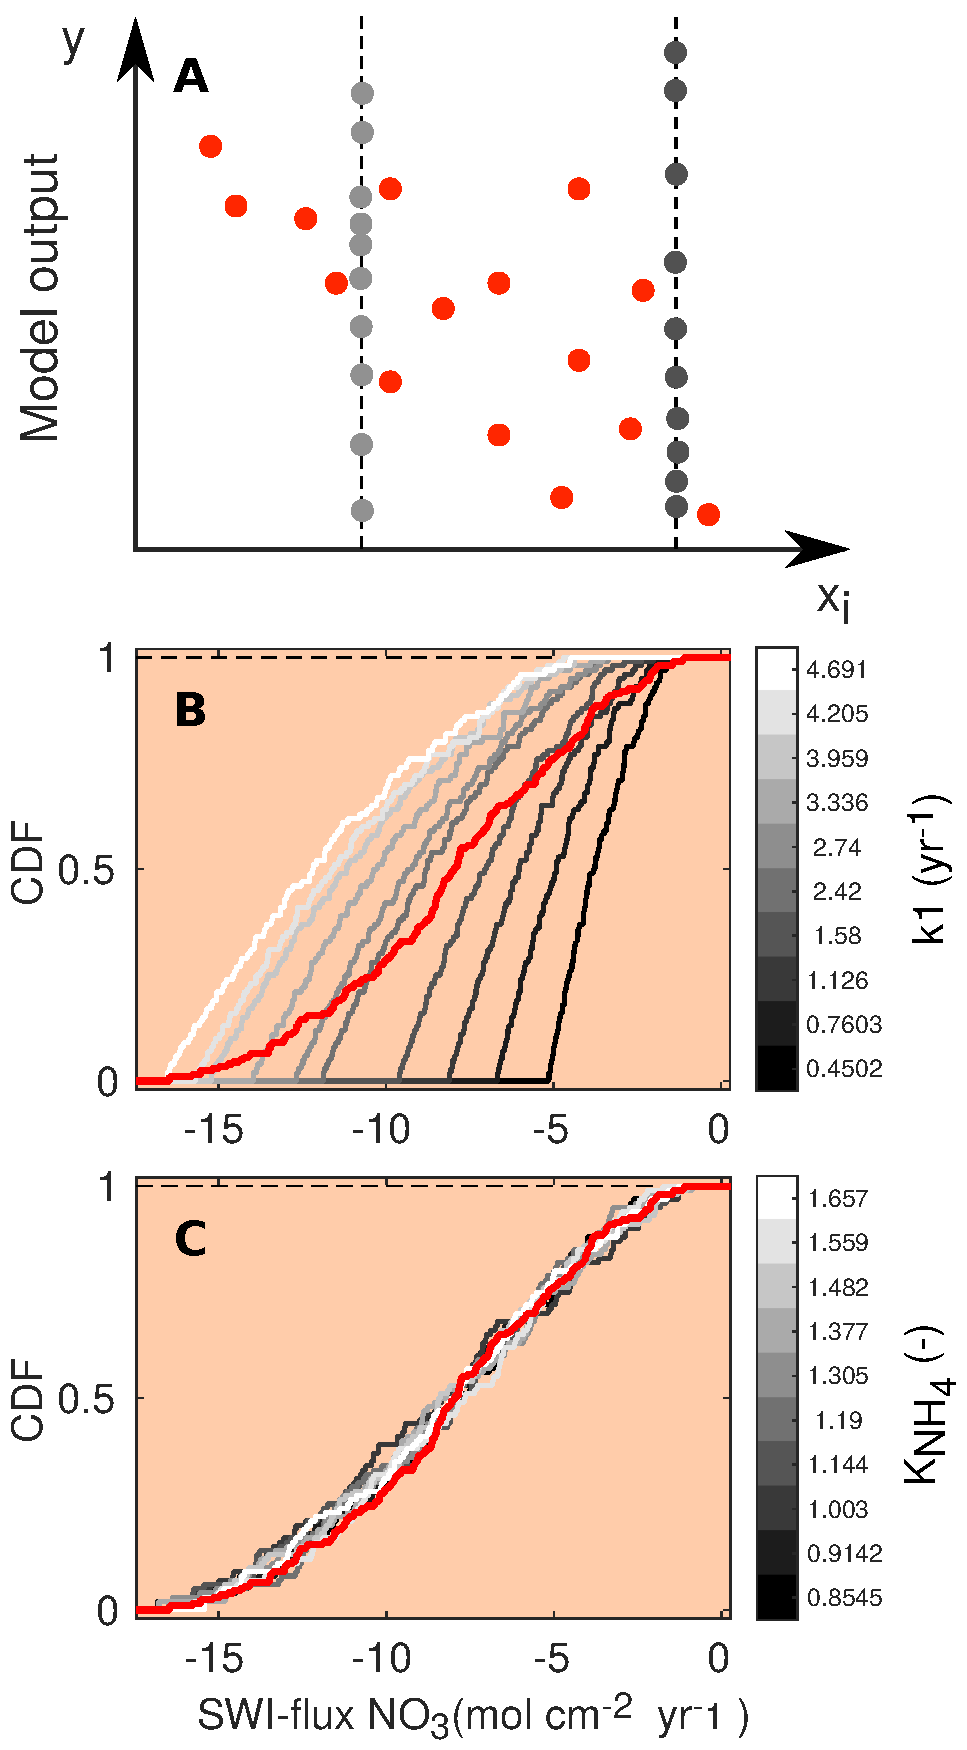
\includegraphics[width=0.6\textwidth]{figures/SA/00_CDFs_400m_NO_3_1807.pdf}
	\caption{A: Schematic of the PAWN method, plotting an uncertain parameter ($x_i$) against a generic model output ($y$). 
	Red dots represent points for calculating the unconditional CDF (NU, here 15), grey dots are points for calculating each conditional CDF (NC, here 10) 
	with n = 2 conditioning points as an example. The user can change the values of NU, NC and n. The number of model evaluations equals $\chem{N_{eval}} = $NU + n$\cdot$NC$\cdot$M, 
	where M is the number of uncertain input parameters. 
	B + C: Two examples of CDFs of the model calculated SWI-flux of \chem{NO_3} using NU = 200, NC = 100 and n = 10. 
	The red lines are the unconditional distribution functions $F_y(\chem{NO_3})$ and the grey lines are the conditional distribution functions $F_{y|x_i}(\chem{NO_3})$ 
	at different fixed values of the input parameters $k_1$ (B) and $K_{\chem{NH_4}}$ (C). 
	As the maximal distance between conditional CDFs and unconditional CDF is greater for $k_1$, this parameter is more influential for the model output 
	(here SWI-flux of \chem{NO_3}, compare Fig. \ref{fig:Sensitivity_Analysis}). 
	}
	\label{fig:Sensitivity_Analysis_methodology}
	\end{center}
\end{figure}

\begin{table}[btp]
\caption{Range of model parameters used for sensitivity analysis of model predicted output.} 
% Note: Constant concentrations at all sites for \chem{SO_4} ($28000 \mu$mol cm$^{-3}$) and \chem{H_2S} (0.0 $\mu$mol cm$^{-3}$).}
\centering
% used for centering table
\begin{tabular}{l l c c c c}
% centered columns (15 columns)
\hline\hline
Parameter & Description & Units & Minimum  & Maximum & Source\\
\hline
$\chem{k_1}$ & labile OM degradation constant & yr$^{-1}$ & $1e^{-4}$ & 5.0 & (1)\\
$\widetilde{\chem{k_2}}$ & order of refractory OM degradation & - & $1e^{-4}$ & $1e^{-1}$ &  (1)\\
 & constant ($k_2 = \widetilde{k_2} \cdot k_1$) & & &  &\\
$\chem{f_1}$ & fraction of labile OM & - & 0.02 & 0.98  & - \\
$K_{\chem{NH_4}}$ & Adsorption coefficient & - & 0.8 & 1.7  & (2) \\
$\gamma_\chem{NH_4}$ & $NH_4$ fraction oxidised &  & 0.5 & 1.0 & - \\
$\gamma_\chem{H_2S}$ &  $H_2S$ fraction oxidised  &  & 0.5 & 1.0 & - \\
$K_\chem{PO_4}^\mathrm{ox}$ & Adsorption coeff. oxic & - & 100.0 & 400.0  & (3) \\
$K_\chem{PO_4}^\mathrm{anox}$ & Adsorption coeff. anoxic & - & 1.3 & 2.0 & (3) \\
$k_{s}$ & kinetic P sorption & yr$^{-1}$  & 0.1 & 100.0 & (4, 5)\\
$k_{m}$ & Fe-bound P release & yr$^{-1}$  & 0.015 & 0.02 & (4, 5)\\
$k_{a}$ & authigenic P formation & yr$^{-1}$  & 0.001 & 10.0 & (4, 6)\\
\hline
Sources: &\multicolumn{5}{l}{(1) \citet{arndt_quantifying_2013}; (2): \citet{cappellen_cycling_1996}; (3): \citet{krom_adsorption_1980}}\\
&\multicolumn{5}{l}{(4): \citet{gypens_simple_2008}; (5): \citet{caroline_p_slomp_key_1996}; (6): \citet{cappellen_mathematical_1988}}
\end{tabular}
\label{table:SA_parameter_ranges}
\end{table}

The PAWN method, as implemented within the Sensitivity Analysis for Everyone (SAFE) matlab toolbox \citep{pianosi_matlab_2015}, is used to investigate M = 11 model parameters for ranges as specified in Table \ref{table:SA_parameter_ranges}. 
Sensitivity indices for all resulting SWI-fluxes for two idealised sediment conditions (i.e. anoxic at 400\,m and oxic at 4000\,m, see Table \ref{table:SA_2Cases}) are calculated. 
We use NU = 200 samples to estimate the unconditional CDF, NC = 100 samples to estimate the conditional CDFs and n = 10 conditioning points. 
Thus as $\chem{N_{eval}}=200+100\cdot10\cdot11$, 11200 model evaluations are performed for each sediment condition. 
The resulting indices are then translated into a color code and summarised in a pattern plot to simplify comparison (Fig. \ref{fig:Sensitivity_Analysis}). 


\begin{table}[btp]
\caption{Model boundary conditions for the two idealised sediment conditions used for the sensitivity analysis (Fig. \ref{fig:Sensitivity_Analysis} and \ref{fig:SA_Color_ScatterPlots}). 
All solute concentrations are in nmol cm$^{-3}$.} 
% Note: Constant concentrations at all sites for \chem{SO_4} ($28000 \mu$mol cm$^{-3}$) and \chem{H_2S} (0.0 $\mu$mol cm$^{-3}$).}
\centering
% used for centering table
\begin{tabular}{c c c c c c c c}
% centered columns (15 columns)
\hline\hline
Depth (m) & Temp. ({}$^\circ$C)& OC (wt\%) & \chem{O_2} & \chem{NO_3} & \chem{SO_4} & \chem{PO_4} & $z_{\mathrm{bio}}$ (cm)\\
\hline
400 & 8.0 & 2.0 & 0.0 & 40.0 & 28,000 & 40.0 & 0.001 \\
4000 & 1.5 & 1.0 & 300.0 & 20.0 & 28,000 & 40.0 & 10.0 \\
\hline
\end{tabular}
\label{table:SA_2Cases}
\end{table}

\subsubsection{Results}
%\section{Sensitivity Analysis}\label{subsec:SA}
Fig. \ref{fig:Sensitivity_Analysis} summarises results of the sensitivity analysis as a colour map. 
Results indicate that generally the most significant parameters for all model outputs are the degradation rate constant for the labile OM pool ($\chem{k_1}$) and the fraction of this pool to the total OM stock ($\chem{f_1}$). 
Other parameters play a minor role for the SWI-fluxes, with the exception of the secondary redox parameters (i.e. $\gamma_\chem{NH_4},\ \gamma_\chem{H_2S}$) in the oxic scenario.
Here, \chem{NH_4}, \chem{SO_4} and \chem{H_2S} are very sensitive to changes in $\gamma_\chem{NH_4}$ and $\gamma_\chem{H_2S}$, as these parameters determine how much of the respective TEA is produced in situ via reoxidation, 
thus affecting the resulting SWI-fluxes. For the oxic scenario, the reoxidation of \chem{H_2S} produced in the sulfidic layer ($\gamma_\chem{H_2S}$, Table \ref{Tab:BC_ALK} Eq. 5) 
also has a strong influence on alkalinity as it decreases alkalinity by 2 moles per mole of \chem{S} oxidized ($\chem{ALK}^\mathrm{H_2S}$, Table \ref{table:reaction_parameters}). 
For the anoxic scenario the secondary redox parameters are essentially non-influential as no \chem{O_2} is available for the reoxidation of reduced substances. 
Especially for the oxic condition the $\chem{PO_4}$ SWI-flux appears to be insensitive to P-related parameters (i.e. $K_\chem{PO_4}^\mathrm{ox}$, $K_\chem{PO_4}^\mathrm{anox}$, $k_s$, $k_m$, $k_a$) as the majority is absorbed to $\chem{Fe}$-oxides. 
The sensitivities change if other $\chem{PO_4}$ related equilibrium concentrations $\chem{PO_4}^s$, $\chem{PO_4}^a$ and $\chem{FeP}^\infty$ are used (not shown).
Overall the results of the sensitivity analysis are in line with what one would expect from a diagenetic model and thus provide ground to confirm that OMEN-SED provides sensible results.

% % \textbf{Sandra: also need to be careful how we formulate it, as you made k2 dependant on k1}. 
% % \textbf{TODO: -frst shortly describe the main results, e.g. fluxes are most sensitivity to variations in OM degradation parameters, other parameters play a secondary role\\
% % the describe which other parameters are red and why\\
% % then describe difference odic-anoxic\\
% % Overall: needs more critical analysis!}

\begin{figure}[htbp]
\begin{center}
	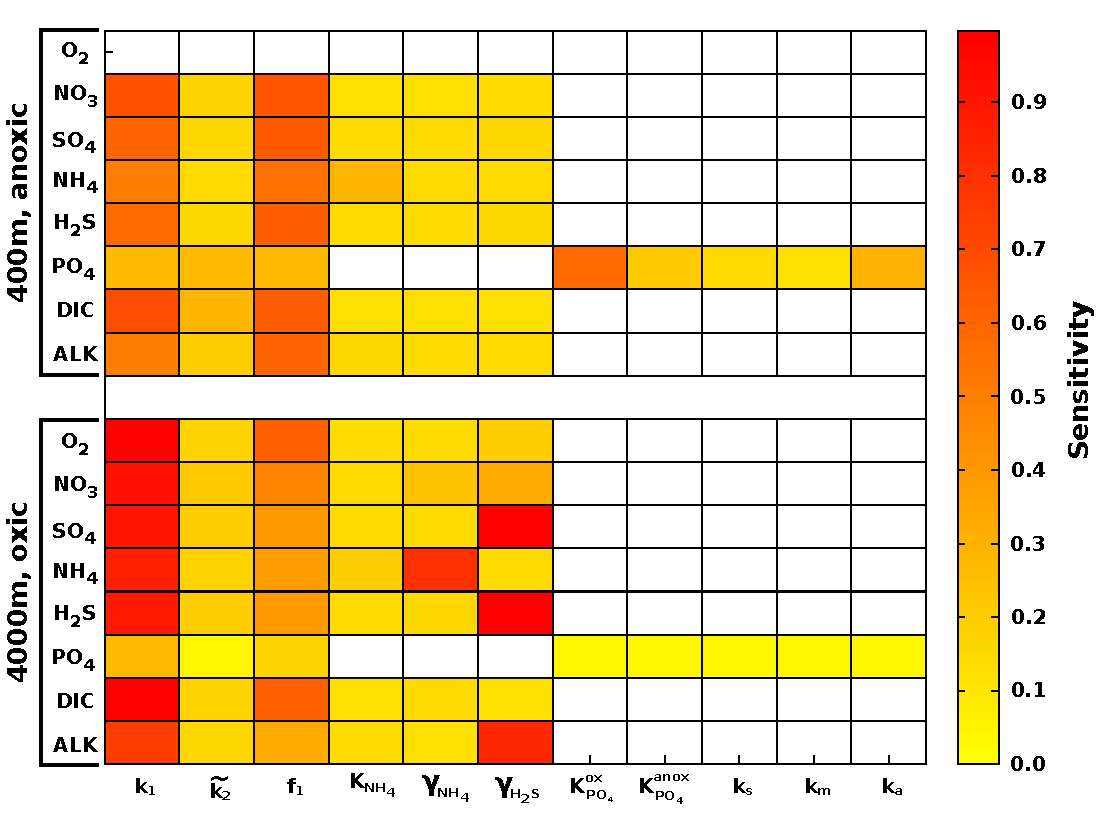
\includegraphics[width=1.0\textwidth]{figures/SA/0_KSIndex_ALL_OUTPUT_13042017.pdf}
	\caption{Pattern plot, showing the output sensitivity for each SWI flux (i.e. the chemical compounds on the vertical axis) and each input factor (i.e. the model parameters 
	on the horizontal axis) for two idealised sediment cores. White patterns are assigned where the SWI flux is independent of the specific parameter. 
	}
	\label{fig:Sensitivity_Analysis}
	\end{center}
%>>>
\marginnote{\textbf{DH}: Rather low PO4 sensitivity - bc of Equil. concentr.?}[-1cm]%<<<
\end{figure}

We further explore the sensitivity of simulated sediment-water exchange fluxes to variations in organic matter degradation parameters by varying $\chem{k_1}$, $\chem{f_1}$ and $\widetilde{\chem{k_2}}$ while all other model 
parameters are set to their default values (Tables \ref{table:sed-charac_transport-parameters} and \ref{table:reaction_parameters}). Minimum and maximum values for $\chem{k_1}$, $\widetilde{\chem{k_2}}$ and $\chem{f_1}$ in 
the shallow ocean are as in Table \ref{table:SA_parameter_ranges}. 
For the deep sea condition we account for the presence of more refractory OM by sampling $\chem{f_1} \in [0.02, 0.3]$, whereas the variation of $\chem{k_1}$ and $\widetilde{\chem{k_2}}$ is as in the shallow ocean. 
The parameter space is sampled using another Latin-Hypercube approach with sample sizes of $N=3500$ for each idealised sediment condition. 
Figure \ref{fig:SA_Color_ScatterPlots} summarises the results of the sensitivity study and the ranges of observed $\chem{O_2}$ and $\chem{NO_3}$ sediment-water interface 
fluxes extracted from a global database \citep{stolpovsky_toward_2015} are indicated on the colour scale. 
Figure \ref{fig:SA_Color_ScatterPlots} shows that the ranges of SWI-fluxes simulated with OMEN-SED are comparable to the observed ranges reported by \citet{stolpovsky_toward_2015}. 
The colour patterns in Figure \ref{fig:SA_Color_ScatterPlots} A and B also reveal the complex interplay between the amount of labile OM \chem{f_1} and its degradation rate \chem{k_1} for the resulting SWI-fluxes 
of \chem{NO_3} in anoxic sediments and \chem{O_2} in aerobic sediments. 
In general, a higher degradation rate in combination with more labile OM available leads to a higher SWI-flux. 
However, higher fluxes extend over a larger range of \chem{k_1}-values when the amount of labile OM \chem{f_1} is high. 
The absence of a colour pattern in Figure \ref{fig:SA_Color_ScatterPlots} C highlights the limited interaction of the two model parameters for \chem{NO_3} SWI-fluxes under oxic conditions. 



\begin{figure}[htbp]
\begin{center}
	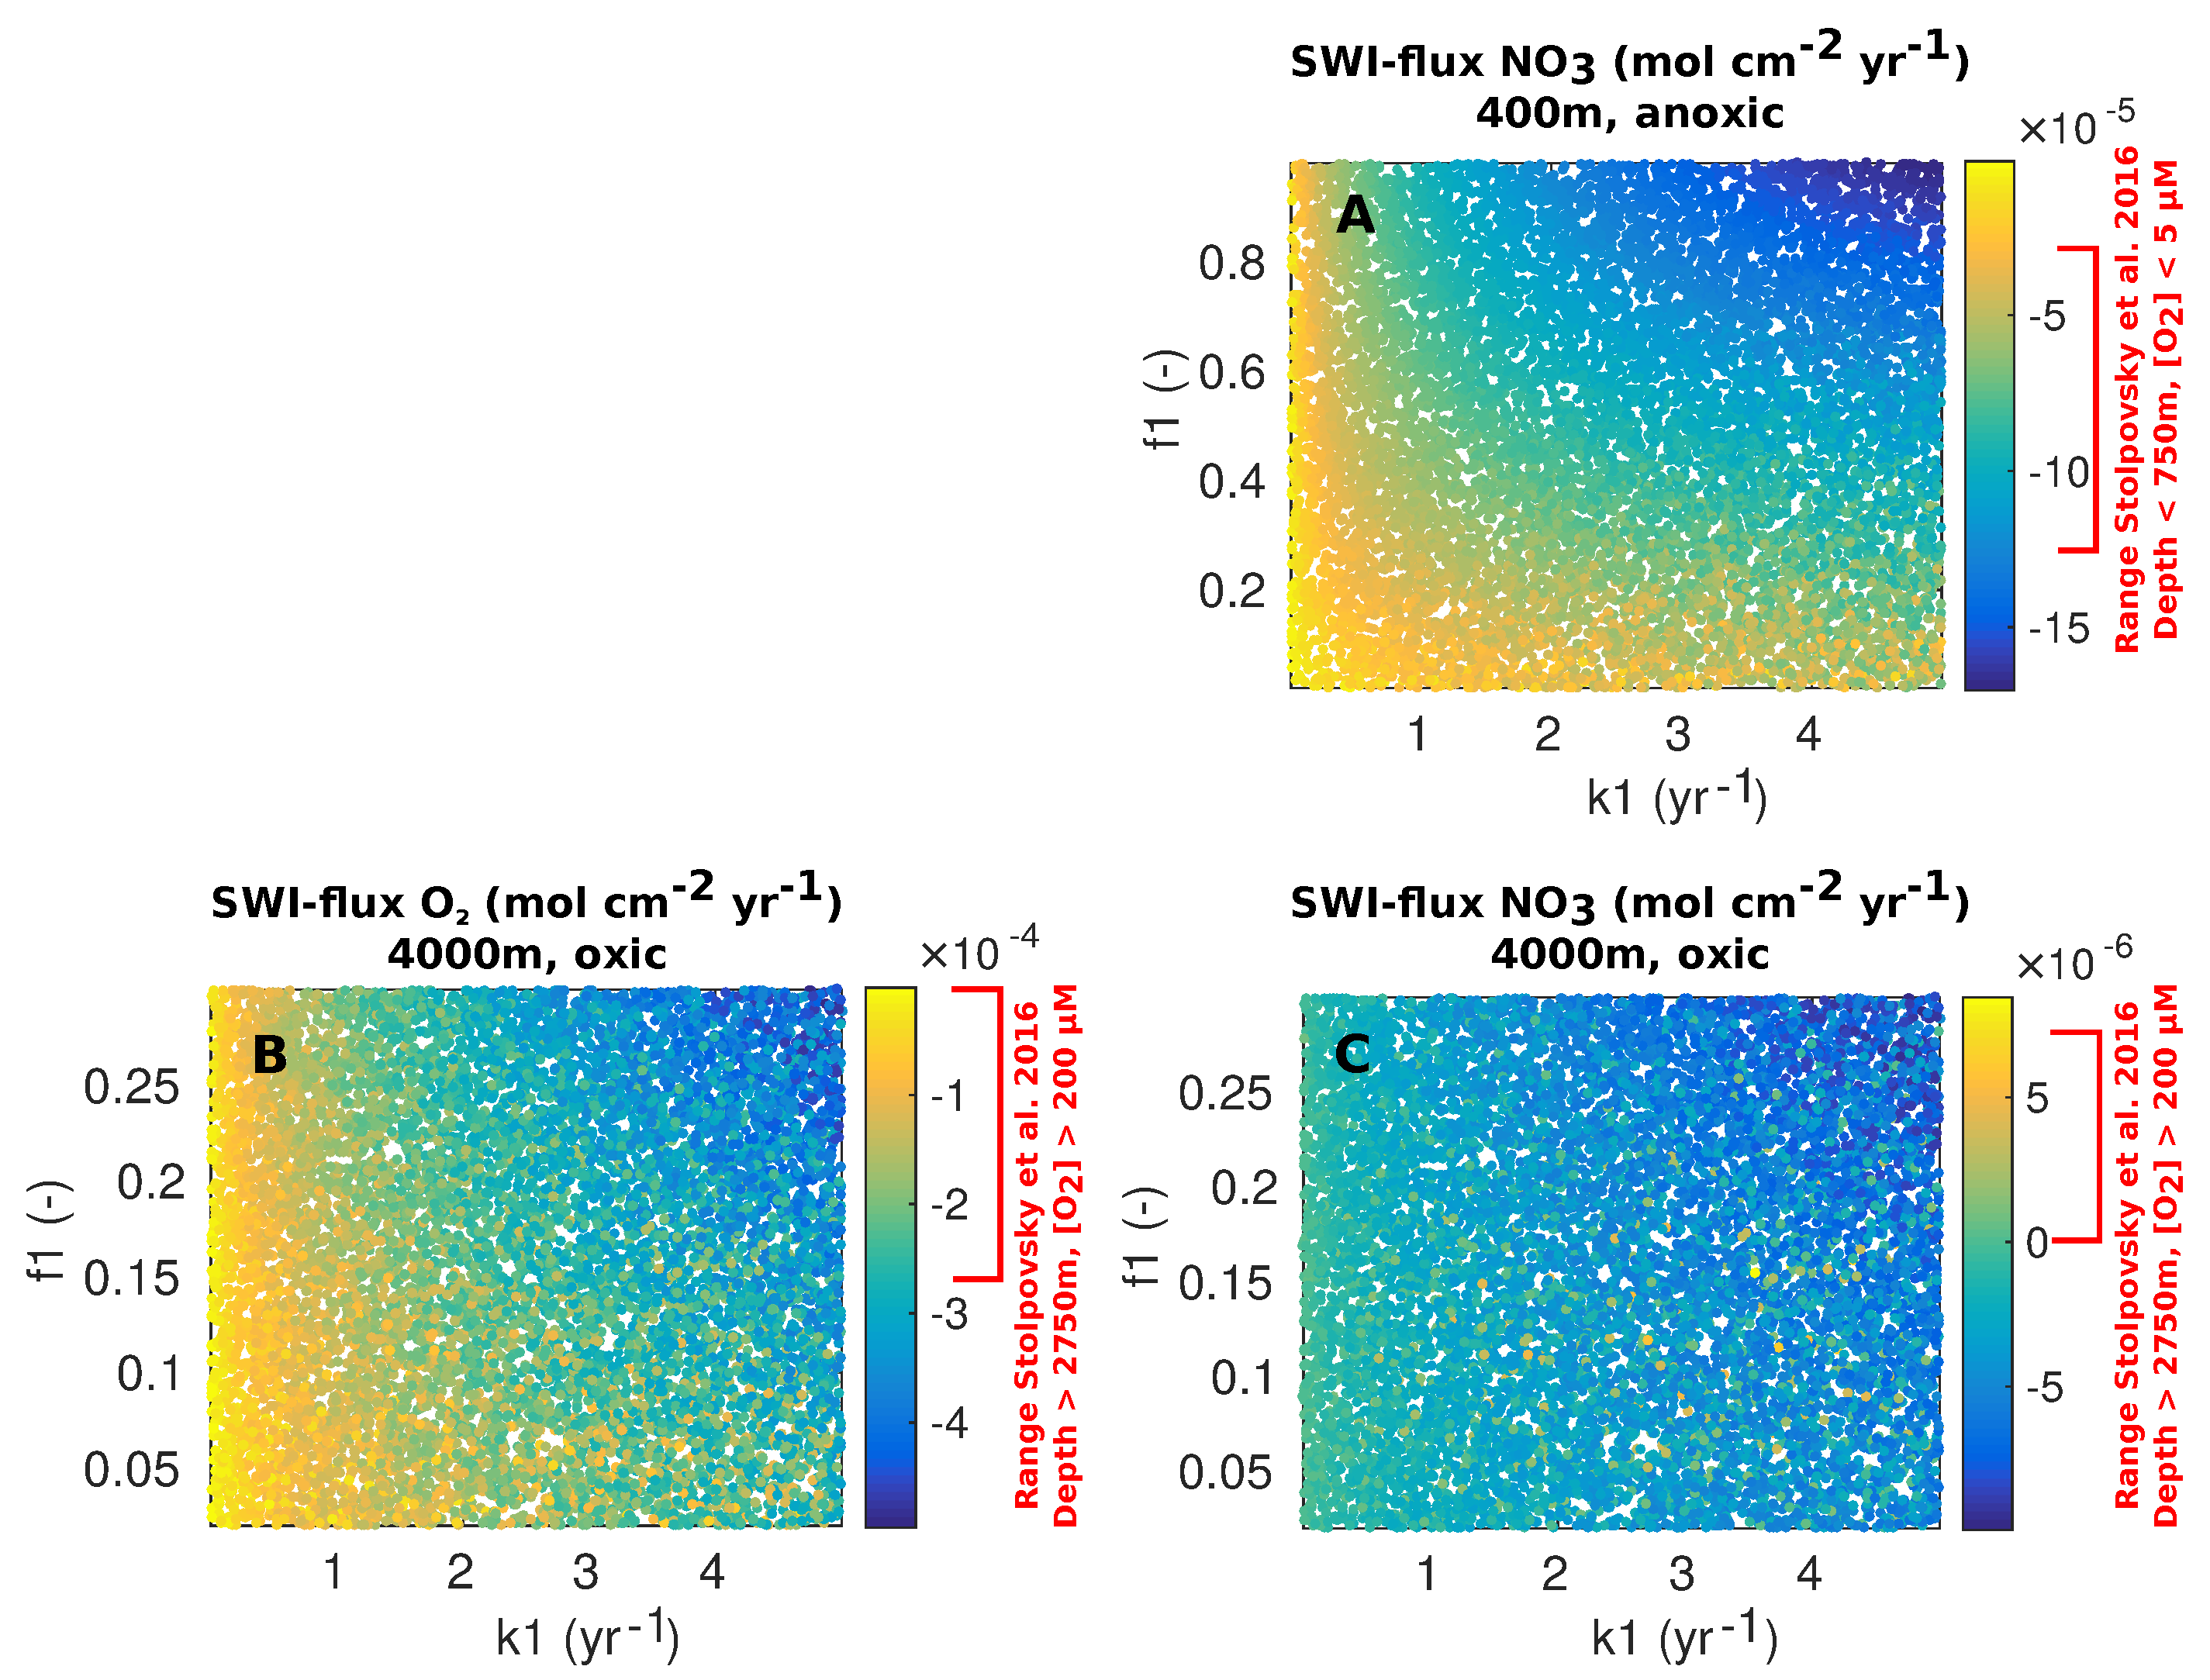
\includegraphics[width=1.0\textwidth]{figures/SA/k1_vs_f1_SWIflux_COMBINED_1604.pdf}
	\caption{Scatter plots ($\chem{k_1}$ vs $\chem{f_1}$) of resulting OMEN-SED SWI-fluxes for the 400m anoxic (A: $\chem{NO_3}$) and 4000m oxic (B: $\chem{O_2}$, C: $\chem{NO_3}$) scenario. 
	Negative values represent a flux from the water column into the sediments.
	Ranges indicated in red on the colour scale correspond to observed benthic fluxes as reported in the global database of \citet{stolpovsky_toward_2015}. 
}\label{fig:SA_Color_ScatterPlots}
% 	%>>>
% \marginnote{\textbf{DH}: Why mainly negative NO3-flux 4000m in contrast to database!?... might change when using diff. gamma}[-6cm]%<<<
\end{center}
\end{figure}


\subsection{Case study: Simulations of sediment cores}\label{subsec:SedProfiles}
\subsubsection{Methodology}
In order to illustrate the capabilities of OMEN-SED, comprehensive datasets from the Santa Barbara Basin \citep{reimers_porewater_1996}, as well as from the Iberian margin and the Nazar\'e Canyon \citep{epping_oxidation_2002} 
are modelled. Modelled profiles are compared with measured pore water data from different depths including the continental shelf (108\,m) and the lower slope (2213\,m) located at the Iberian margin,
the upper slope (585\,m) from the Santa Barbara Basin, and a deep sea site (4298\,m) in the Nazar\'e Canyon. 
The Santa Barbara Basin is characterised by anoxic bottom waters, high POC concentrations and varved sediments \citep{reimers_seasonal_1990}, therefore the depth of bioturbation in OMEN-SED 
is restricted to the upper 0.01 cm. In the uppermost sediments iron(III) hydroxides are reduced, releasing \chem{Fe^{2+}} which reacts with sulfide to form iron sulfides. 
Thus, the \chem{Fe} cycle exerts a strong control on sulfide concentrations in the sediments of this basin \citep{reimers_porewater_1996}. 
In addition, the sediments are generally supersaturated with respect to carbonate fluorapatite by and below 2 cm \citep{reimers_porewater_1996}. 
The Iberian margin, situated in the northeastern Atlantic, generally belongs to the more productive regions of the global ocean \citep{longhurst_estimate_1995}, however, seasonal changes in upwelling creates a strong temporal variability in 
primary productivity and organic carbon deposition. Submarine canyons in this area (like the Nazar\'e Canyon) may deliver organic carbon from the shelf to the ocean interior \citep{van_weering_recent_2002, epping_oxidation_2002}.
For a more detailed description of the study areas and the experimental work, the interested reader is referred to the publications by \citet{reimers_porewater_1996} and \citet{epping_oxidation_2002}. 

In OMEN-SED sediment characteristics and boundary conditions are set to the observed values where available (Table \ref{table:Profiles_BC}). Other sediment characteristics (e.g. sedimentation rate, porosity, density), 
stoichiometric factors and secondary reaction parameters are set to the default value (see Tables \ref{table:sed-charac_transport-parameters} and \ref{table:reaction_parameters}).
Organic matter is modelled as two fractions, with different first-order degradation rate constants. 
The POC and pore water profiles were fitted by optimizing the POC partitioning into the fast and slow degrading pool and their respective first-order degradation rate constants (priority is given to reproduce the POC 
and \chem{O_2} profiles). For phosphorus the equilibrium concentration for authigenic P formation (\chem{PO_4^a}) was adjusted to fit the \chem{PO_4} concentration at $z_\infty$. 

\begin{table}[btp]
\caption{Model boundary conditions for the simulated sediment profiles in the Santa Barbara basin (108 and 2213 m) and Iberian margin (585 and 4298 m) reported in Figure \ref{fig:Sediment_profiles}. For all sites a DIC bottom water concentration of 
2,400 nmols cm$^{-3}$ is assumed.} 
% Note: Constant concentrations at all sites for \chem{SO_4} ($28000 \mu$mol cm$^{-3}$) and \chem{H_2S} (0.0 $\mu$mol cm$^{-3}$).}
\centering
% used for centering table
\begin{tabular}{l c c c c c c c c} 
% centered columns (15 columns)
\hline\hline
\multicolumn{8}{l}{\textbf{Sediment characteristics:}}\\
Depth & Temp. & $z_{\mathrm{bio}}$ & $D_{\mathrm{bio}}$  & \chem{POC_1} & \chem{POC_2} & \chem{k_1} & \chem{k_2}\\
 (m) & ($^{\circ}$C) & (cm) & (cm$^2$yr$^{-1}$) &(wt\%) & (wt\%) & (yr$^{-1}$) & (yr$^{-1}$)\\
\hline
108 & 12.5 & 1.0 & 0.02 & 2.64 & 1.8 & 0.65 & $1.0e^{-5}$ \\
585 & 5.85 & 0.01 & 0.02 & 2.0 & 3.5 & 0.2 & $8.0e^{-4}$\\
2213 & 3.2 & 10.0 & 0.17 & 0.45 & 0.5 & 0.1 & $4.0e^{-4}$\\
4298 & 2.5 & 4.2 & 0.18 & 0.83 & 1.2 & 0.052 & $1e^{-5}$\\
\hline\hline
\multicolumn{8}{l}{\textbf{Bottom water concentrations of solutes} (all in nmol cm$^{-3}$):}\\
Depth & \chem{O_2} & \chem{NO_3} & \chem{SO_4} & \chem{NH_4} & \chem{H_2S} & \chem{PO_4} & \chem{PO_4^a} & \chem{Alkalinity}\\
%(m) & ($\frac{\mu mol}{cm^3}$) &  ($\frac{\mu mol}{cm^3}$) &  ($\frac{\mu mol}{cm^3}$) &  ($\frac{\mu mol}{cm^3}$) &  ($\frac{\mu mol}{cm^3}$)  &   ($\frac{\mu mol}{cm^3}$) &   ($\frac{\mu mol}{cm^3}$) \\
\hline
108 & 210 & 9.6 & 28,000 & 0.4 & 0.0 & 0.0 & 15.0 & 2,400\\
585 & 10 & 25.0 & 28,000 & 0.0 & 0.0 & 50.0 & 90.0 & 2,480\\
2213 & 250 & 25.0 & 28,000 & 0.6 & 0.0 & 0.0 & 5.0 & 2,400\\
4298 & 243 & 30.1 & 28,000 & 0.22 & 0.0 & 0.0 & 5.0 & 2,400\\
% inserts double horizontal lines
\end{tabular}
\label{table:Profiles_BC}
\end{table}

\subsubsection{Results}
%\subsection{Stand-alone simulation of sediment cores}\label{subsec:SedProfiles}
Fig. \ref{fig:Sediment_profiles} compares modelled and observed sediment profiles for the Santa Barbara Basin and the Iberian margin. Results show 
that OMEN-SED is able to capture the main diagenetic features across a range of different environments without changing model parameters (e.g. stoichiometric ratios or secondary reaction parameters) to site specific conditions. 
For the two open Iberian margin stations (108 and 2213 m) OMEN-SED fits all observations well. OMEN-SED does especially well at seafloor depth (SFD) 2213 m by reproducing the deep \chem{O_2} penetration and the subsurface maximum in \chem{NO_3} 
concentration due to the nitrification of \chem{NH_4} (note, that \chem{NH_4} is overestimated at this SFD). 
For the anoxic Santa Barbara Basin (585 m) the decrease in \chem{SO_4} and the increase in \chem{ALK} concentration with sediment depth is well represented, indicating the 
importance of sulfate reduction as the primary pathway of OM degradation at this site \citep[compare with][]{meysman_reactive_2003}. 
However, a misfit is observed for \chem{H_2S} and \chem{PO_4} in the upper 20 cm of this sediment core. The discrepancy for \chem{H_2S} can be explained by high iron(III) hydroxide concentrations, 
which is reduced to degrade organic matter (especially in the $2-4$ cm depth interval), therefore placing the beginning of the sulfate reduction zone and the production of \chem{H_2S} to the deeper sediments \citep{reimers_porewater_1996}. 
Iron processes are currently not dynamically represented in OMEN-SED. 
In addition, produced dissolved \chem{Fe} reacts with \chem{H_2S} to form iron sulfides (e.g. pyrite, \chem{FeS_2}) and thus further inhibits the rise of \chem{H_2S} \citep{reimers_seasonal_1990}. 
The iron cycle also plays a critical role for phosphorus, as the reduction of iron(III) hydroxides in the surface sediments releases sorbed phosphate, leading to pore waters around and below 2 cm which are supersaturated with 
respect to fluorapatite, thus initiating \chem{CFA} precipitation. \citet{reimers_porewater_1996} could even show that the accumulation of \chem{CFA} is mainly restricted to the near-surface sediments ($\sim 5$ cm) 
instead of throughout the sediment column. % throughout the sediment column: Ruttenberg and Berner, 1993
As OMEN-SED does not include an iron-cyle, and Fe-bound P and \chem{CFA} processes are highly parameterised, the model is not able to capture these complex, non-steady state phosphorus 
dynamics at this specific site. 
For the Nazar\'e Canyon station (4298 m) satisfactory fits could be realised apart from \chem{NH_4}. However, also \citet{epping_oxidation_2002} could not obtain a better fit 
using a more complex diagenetic model. They suggested non-local solute exchange resulting from bioirrigation being responsible for the higher \chem{NH_4} concentrations at this site which is neglected in their model, as well as in 
OMEN-SED. Furthermore, the fractured POC profile (indicating episodic depositional events through the canyon) could have been approximated using a different partitioning of the bulk POC into 
labile and refractory pool with different degradation rate constants, thus potentially leading to a better fit of the \chem{NH_4} profile.  
In general, better approximations of the data could have potentially been acquired by applying a sensitivity study using different NC-ratios \citep[e.g.][report different ratios from Redfield stoichiometry]{epping_oxidation_2002} 
and exploring the parameter space for the secondary reaction parameters ($\gamma_{NH_4}$, $\gamma_{H_2S}$). 
However, considering these generalisations and our assumption of steady-state, which might not be valid, particularly for the complex Santa Barbara basin, the shallow core and the Nazar\'e Canyon, which are affected by seasonality 
and biology, OMEN-SED performs well in capturing the main diagenetic processes. 

\begin{sidewaysfigure}[tbp]
	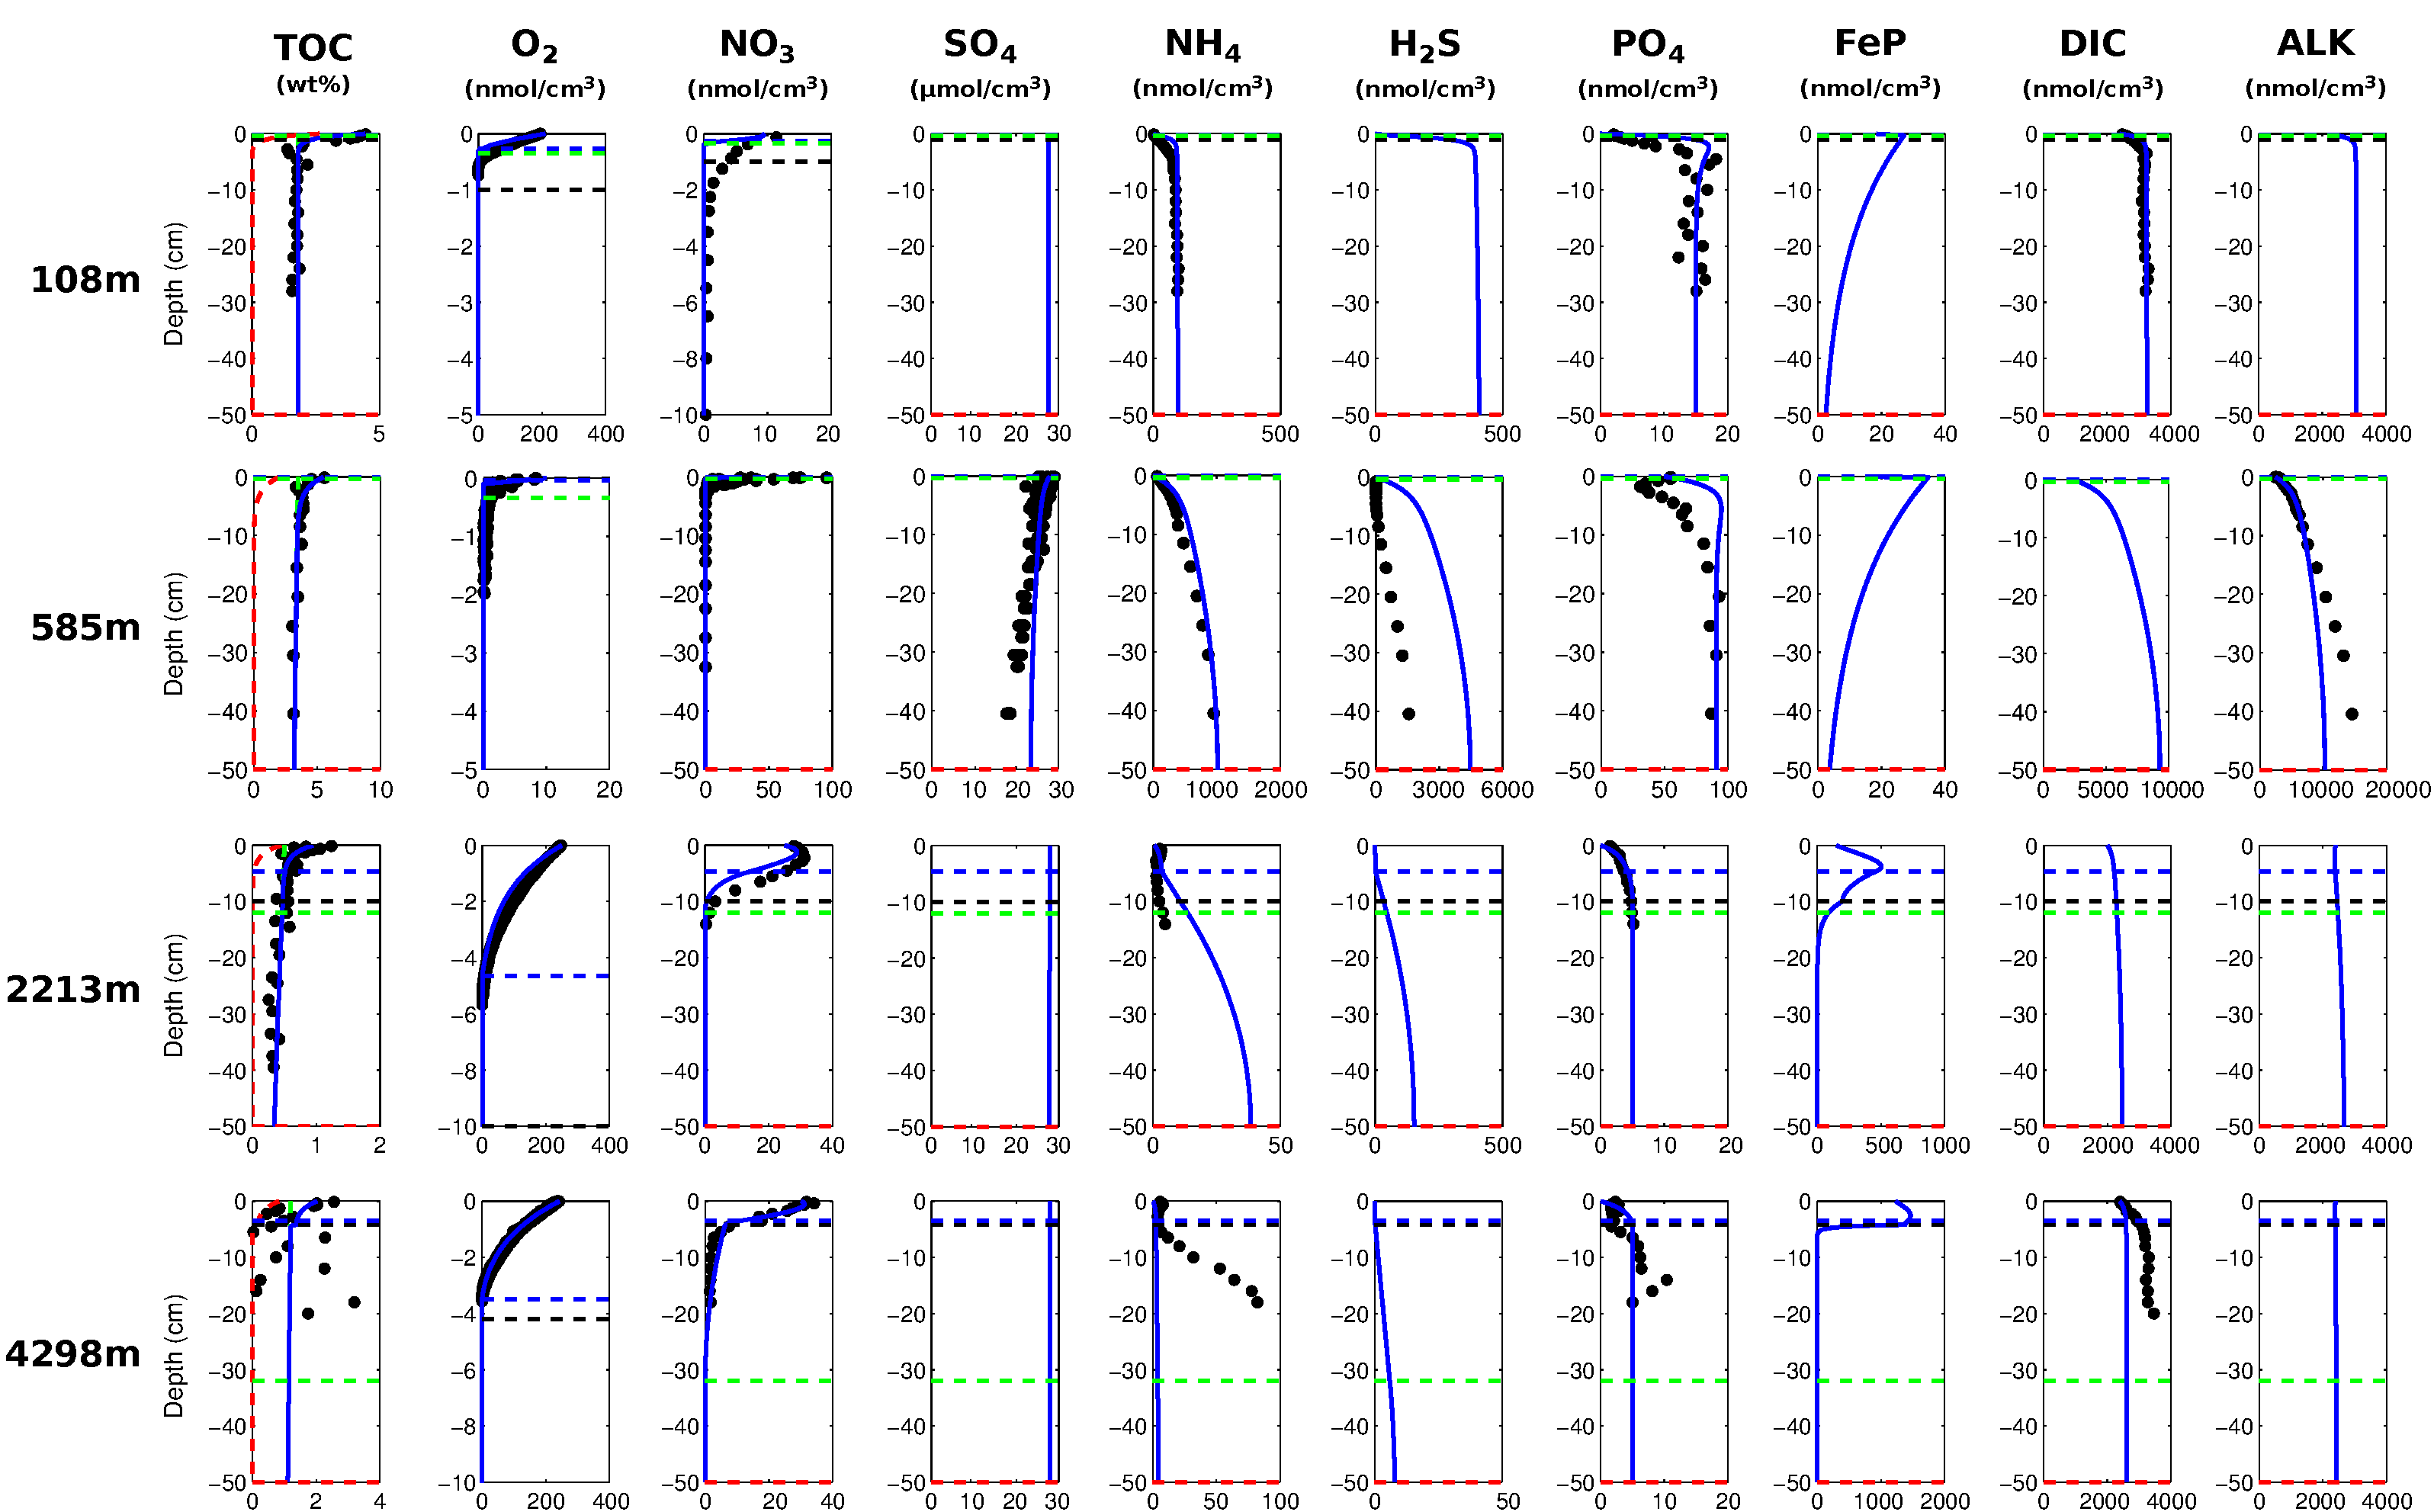
\includegraphics[width=1.0\textwidth]{figures/Profiles/0_ALL_PROFILES_COMBINED_1503.pdf}
	\caption{Modelled (curves) and measured (filled dots) solid phase and dissolved pore water profiles for four different sediment cores. Note that different 
	scales are used for different stations. The blue POC curve represents the sum of the refractory (green) and labile (red) POC fraction. The horizontal dashed lines in each panel indicate the 
	bioturbation depth (black) and the penetration depths of oxygen (blue), nitrate (green) and sulfate (red) as calculated by OMEN-SED.}
	\label{fig:Sediment_profiles}
\end{sidewaysfigure}


\subsection{Case study: Stand-alone simulations of global ocean transect}\label{subsec:globalhypsometry}
\subsubsection{Methodology}
In this section it is tested to which degree OMEN-SED is capable of capturing the dynamics of organic matter degradation pathways and related TEA-fluxes as simulated with a complete, numerical diagenetic model. 
Therefore, we reproduce the simulations of typical conditions along a global ocean hypsometry of \citet{thullner_global_scale_2009} and compare our modelled TEA-fluxes with the results of the complete model as well as with 
observations from \citet{middelburg_denitrification_1996}. To explore the global degradation of OM in the seafloor 
\citet{thullner_global_scale_2009} quantified various diagenetic processes using the Biogeochemical Reaction Network Simulator \citep[BRNS,][]{aguilera_knowledge-based_2005}, 
a flexible simulation environment suitable for reactive transport simulations of complex biogeochemical problems \citep[e.g.][]{jourabchi_quantitative_2005, thullner_modeling_2005}. 
\citet{thullner_global_scale_2009} used seafloor depth (SFD) as the master variable and calculated model parameters, such as $w$, $D_{bio}$ and $\phi$, from existing empirical relationships 
\citep[e.g.][]{van1995metal, middelburg_empirical_1997}. 
Organic matter degradation was described with a 1-G approach, thus assuming a single pool of organic matter of uniform reactivity. 
The first order rate constant was related to the burial velocity, $w$ (cm year$^{-1}$), following the empirical relationship of \citet{boudreau1997diagenetic}:
\begin{equation}
 k=0.38\cdot w^{0.59}.
\end{equation}
This rate constant can be assumed as the mean reactivity of the organic matter fractions which are degraded in the upper, bioturbated $10-20$ cm of the sediments. 
Thus, more reactive fractions (degraded during days/weeks close to the SWI) and more refractory fractions (degraded on longer time scales deeper in the sediments) are not captured by this relationship \citep{boudreau1997diagenetic}. 
BRNS simulations were performed using boundary conditions and parameters for depths representative for shelf, slope and deep sea sediments (i.e. SFD of 100m, 200m, 500m, 1000m, 2000m, 3500m and 5000m). 
In order to reproduce these results, OMEN-SED is configured here as a 1-G model and boundary conditions and model parameters are defined as in \citet[][see Table \ref{table:Hypsometry_params}]{thullner_global_scale_2009}. 
As OMEN-SED assumes a fixed fraction of reduced substances to be reoxidised, which exerts a large impact on the resulting SWI-fluxes (compare Section \ref{subsec:SA}), 
two sets of simulations are performed in order to show the range of possible model outputs. In the first setup 95\% of the reduced substances are reoxidised (i.e. $\gamma_{NH_4}=\gamma_{H_2S}=0.95$) and in the 
second only 5\% are reoxidised (all other model parameters and boundary conditions are equal). 
\begin{table}[hbtp]
\caption{Seafloor depth dependency of key model parameters and boundary conditions \citep[adapted from][]{thullner_global_scale_2009}.} 
% Note: Constant concentrations at all sites for \chem{SO_4} ($28000 \mu$mol cm$^{-3}$) and \chem{H_2S} (0.0 $\mu$mol cm$^{-3}$).}
\centering
% used for centering table
\begin{tabular}{c c c c c c c c} 
% centered columns (15 columns)
\hline
& \multicolumn{7}{c}{\textbf{Seafloor depth}}\\
\cline{2-8}
 & 100 m & 200 m & 500 m  & 1000 m & 2000 m & 3500 m & 5000 m\\
\hline
\multicolumn{1}{l}{\textbf{Model parameters}}\\
 $w{}^a$ (cm yr$^{-1}$) & $3.98 \times 10^{-1}$ & $ 3.60 \times 10^{-1}$ & $ 2.67 \times 10^{-1}$ & $ 1.62 \times 10^{-1}$ & $5.94  \times 10^{-2}$ & $ 1.32 \times 10^{-2}$ & $ 2.94 \times 10^{-3}$\\
 $D_{\mathrm{bio}}{}^a$ (cm$^2$ yr$^{-1}$) & 27.5 & 25.1 & 19.0 & 12.1 & 4.83 & 1.23 & 0.310\\
 $\phi^b$ & 0.85 & 0.85 & 0.80 & 0.80 & 0.80 & 0.80 & 0.80\\
 T${}^c$ ($^{\circ}$C) & 10.3 & 9.7 & 8.1 & 5.8 & 3.0 & 1.5 & 1.4\\
 $\rho_{\mathrm{sed}}{}^c$ (g\,cm$^{-3}$) & 2.5  & 2.5 & 2.5 & 2.5 & 2.5 & 2.5 & 2.5\\
 $k^d$ (yr$^{-1}$) & 0.221 & 0.208 & 0.174 & 0.130 & 0.0718 & 0.0296 & 0.0122\\
\multicolumn{1}{l}{\textbf{Upper boundary conditions}}\\
\chem{POC_{flux}}$^a$ ($\mu$mol cm$^{-2}$yr$^{-1}$) & 510 & 467 & 357 & 228 & 93.0 & 24.3 & 6.33\\
\chem{POC}$^e$ (wt\%) & 0.79 & 0.78 & 0.55 & 0.50  & 0.42 & 0.32 & 0.25\\
\chem{O_{2,0}}$^c$ (nmol cm$^{-3}$) & 132 & 129 & 121 & 114 & 116 & 135 & 141\\
\chem{NO_{3,0}}$^c$ (nmol cm$^{-3}$) & 17.3 & 18.6 & 22.1 & 26.5 & 31.0 & 31.6 & 31.6\\
\chem{SO_{4,0}}$^b$ (nmol cm$^{-3}$) & 28,000 & 28,000 & 28,000 & 28,000 & 28,000 & 28,000 & 28,000\\
\hline
\multicolumn{3}{l}{${}^a$ Derived from \citet{middelburg_empirical_1997}.}	& \multicolumn{5}{l}{${}^b$ Derived from \citet{van1995metal}.}\\
\multicolumn{3}{l}{${}^c$ Derived from \citet{conkright2002world}.}		& \multicolumn{5}{l}{${}^d$ Derived from \citet{boudreau1997diagenetic}.}\\
\multicolumn{3}{l}{${}^e$ Calculated with OMEN-SED from \chem{POC_{flux}}.}
% inserts double horizontal lines
\end{tabular}
\label{table:Hypsometry_params}
\end{table}

\subsubsection{Results}
%\subsection{Stand-alone simulations of global ocean transect}\label{subsec:globalhypsometry}
%Figure \ref{fig:hypsometry} (A-C) compares simulated depth-integrated organic matter mineralisation rates ($\mu$mol C cm$^{-2}$\,yr$^{-1}$) by three degradation pathways along the global hypsometry. 
Figure \ref{fig:hypsometry} compares simulated SWI-fluxes of TEAs (i.e. \chem{O_2}, \chem{NO_3} and \chem{SO_4}) along the global hypsometry using OMEN-SED (black lines) with the results of \citet{thullner_global_scale_2009} 
(red lines). 
Observations for \chem{O_2} and \chem{NO_3} fluxes are taken from \citet{middelburg_denitrification_1996}. 
% Also plotted in Fig. \ref{fig:hypsometry}A are the total oxygen uptake (TOU) estimates presented in \citet{thullner_global_scale_2009} (filled red symbols), who assumed the organic matter flux to be equivalent to TOU. 
Due to the applied empirical relations organic matter flux to the seafloor decreases by 2 orders of magnitude from 100 to 5000 m and its degradation rate constant by 1 order of magnitude (Table \ref{table:Hypsometry_params}). 
Therefore, the rate of organic matter degradation is about 50 times greater at 100 m than at 5000 m \citep[compare][]{thullner_global_scale_2009}, thus resulting in a decrease of TEA-fluxes along the 
hypsometry (Figure \ref{fig:hypsometry}). 
% actual OMEN values are weird: Therefore, the rate of organic matter degradation is about 15 times greater at 100 m (2765 $\mu$mol cm$^{-2}$ yr$^{-1}$) than at 5000 m (175 $\mu$mol cm$^{-2}$ yr$^{-1}$), thus resulting in a decrease of TEA-fluxes along the hypsometry (Figure \ref{fig:hypsometry}). 
The 95\%-reoxidation experiments (dots) show proportionally higher \chem{O_2} in-fluxes than the the 5\%-reoxidation experiments (triangles) because more \chem{O_2} is utilised for 
in situ production of \chem{NO_3} and \chem{SO_4} in the sediments. This is also mirrored by the increased \chem{NO_3} out-flux and decreased \chem{SO_4} in-flux for shallower SFDs. 
This is in line with the results of \citet{thullner_global_scale_2009} which showed that in situ production is an important pathway of \chem{SO_4} supply in the sediment, which is responsible for $\sim$80\% of the total OM degradation at depths 
between 100 and 2000 m (\chem{SO_4} is not used for OM degradation in OMEN-SED below 2000m).
In general, Figure \ref{fig:hypsometry} shows that OMEN-SED captures the main trends in observed TEA fluxes well and fluxes calculated with BRNS fall within the range of possible OMEN-SED results. 
\begin{figure}[htbp]
\begin{center}
	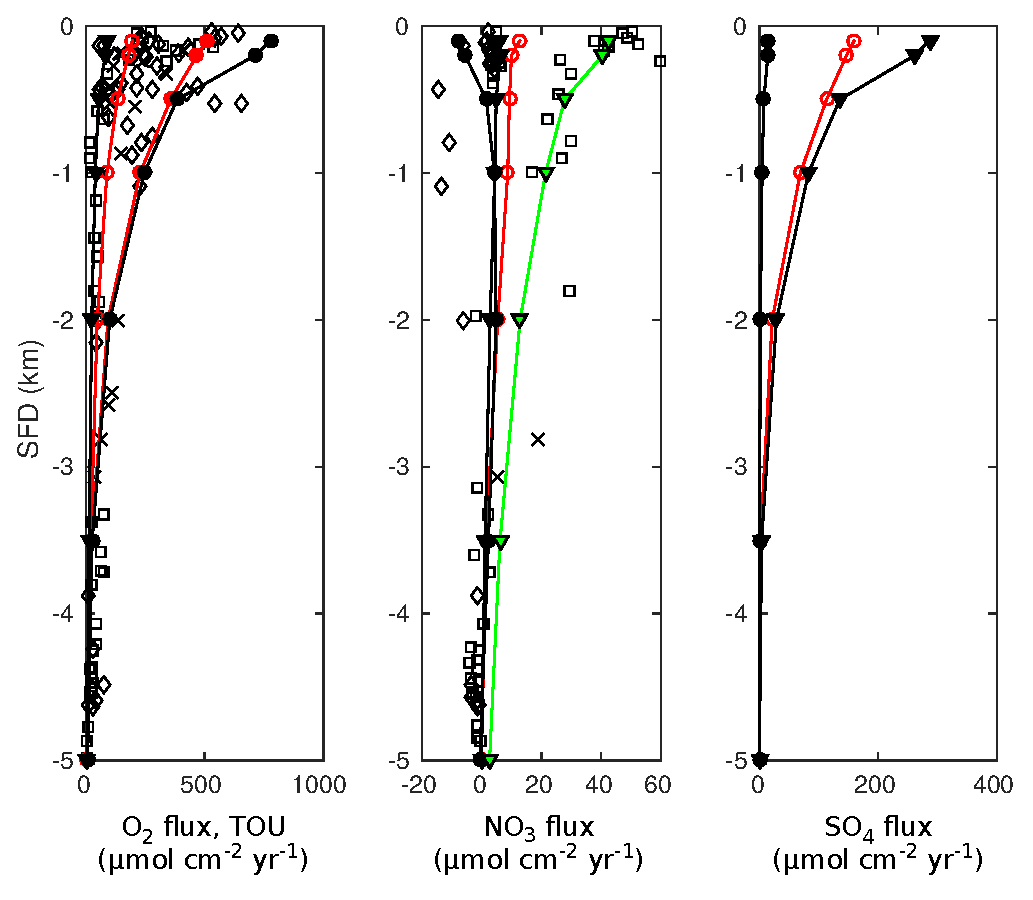
\includegraphics[width=0.8\textwidth]{figures/0_OMEN_Thullner_hypsometry_fluxes_diff_NCratio.pdf}
	\caption{Fluxes of \chem{O_2}, \chem{NO_3} and \chem{SO_4} to the sediment along the global hypsometry. 
	Red lines (with open symbols) are modelled fluxes from \citet{thullner_global_scale_2009} using BRNS; black lines are results from OMEN-SED ($\bullet$ : $\gamma_{NH_4}=\gamma_{H_2S}=0.95$; 
	$\blacktriangledown$: $\gamma_{NH_4}=\gamma_{H_2S}=0.05$). 
	Observations of TEA fluxes are taken from \citet{middelburg_denitrification_1996} ($\Diamond$: Atlantic, $\square$: Pacific, $\times$: Arctic/Indian Ocean). 
	Also plotted in Figure (A) are the total oxygen uptake (TOU) estimates of \citet{thullner_global_scale_2009} (filled red symbols). The green line indicates OMEN-SED results for low oxygen/high nitrate levels and the lower 
	NC-ratio. Negative values are directed out of the sediments.
	}\label{fig:hypsometry}
\end{center}
\end{figure}

In particular, the observed \chem{O_2} fluxes in the upper 2000m are well predicted by the two OMEN-SED simulations. Oxygen fluxes for the deep-sea sediments, however, are slightly underestimated. 
These deviations can presumably be related to the assumed 1-G description of organic matter degradation, which neglects the more labile OM pool. This highly reactive pool is degraded close to the sediment surface, 
thus promoting higher aerobic degradation rates and higher \chem{O_2} fluxes.  
Nitrate fluxes in the upper 500m of the Atlantic Ocean are well predicted. However, as in \citet{middelburg_denitrification_1996} the direction of calculated nitrate fluxes in the upper 1000m of the Pacific Ocean differ from the observations. 
\citet{middelburg_denitrification_1996} related these discrepancies to the globally averaged model parameters and the applied boundary conditions. They could reduce the disagreements significantly by using more representative 
bottom water concentrations for the eastern Pacific and a higher flux of labile organic matter for their 2-G model. By changing the boundary conditions and the NC-atomic ratio of organic matter for the whole hypsometry, it is possible 
to obtain a better model-data fit with OMEN-SED for the shallow Pacific Ocean (green line in Fig. \ref{fig:hypsometry}B). 
\citet{bohlen_simple_2012} report that the atomic NC-ratio strongly deviates from Redfield stoichiometry (0.151) with specifically lower values for the East Pacific Ocean. The use of their globally averaged value of 0.067 allows 
reconciling modelled and observed values provided that bottom water conditions are also changed to the low oxygen/high nitrate levels more likely to be found in the shallow Pacific Ocean 
($\chem{O_2} = 10$ nmol cm$^{-3}$ and $\chem{NO_3} = 80$ nmol cm$^{-3}$). 


\section{Coupled pre-industrial Earth system model simulations}\label{sec:ESM_coupling}
\subsection{Coupling to the cGENIE Earth system model}\label{subsubsec:Methods_ESM_coupling}
% Describe what needs to be done/checked. Compare/use as example what I did with GENIE coupling. What are the if-clauses used? Input to OMEN-SED, output of OMEN-SED. 
\begin{figure}[tbp]
\begin{center}
	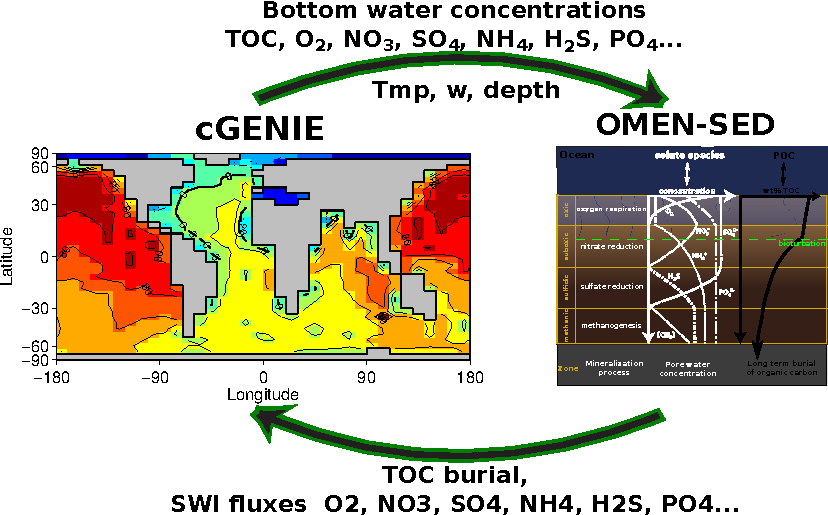
\includegraphics[width=0.8\textwidth]{figures/OMEN-GENIE-coupling.pdf}
	\caption{Schematic of the relationship between OMEN-SED and cGENIE. Arrows and accompanied text represent the information transferred between models. }
	\label{fig:OMEN-GENIE-coupling}
	\end{center}
\end{figure}
OMEN-SED is coupled to the carbon-centric version of the ``GENIE'' Earth system model \citep[cGENIE,][]{ridgwell_marine_2007} to illustrate the abilities of the newly developed model. 
The following section provides a brief description of cGENIE and the coupling procedure (Fig. \ref{fig:OMEN-GENIE-coupling}). 
cGENIE is a model of Intermediate Complexity based on the efficient climate model ``C-GOLDSTEIN''  of \citet{edwards_uncertainties_2005}, featuring a frictional-geostrophic 3D-ocean circulation model coupled to a fast 
Energy-Moisture Balance 2D-atmosphere together with a dynamic-thermodynamic sea-ice component. 
The version of cGENIE used here includes the marine geochemical cycling of carbon, oxygen, phosphorus and sulfur \citep{ridgwell_marine_2007}, 
preservation of carbonates in deep-sea sediments \citep[SEDGEM,][]{ridgwell_regulation_2007} and terrestrial weathering \citep{colbourn_rock_2013}. 
The ocean model is implemented on a 36$\times$36 equal-area horizontal grid with 16 vertical levels using the pre-industrial continental configuration and bathymetry as in \citet{archer_atmospheric_2009}. 
A finer grid (72$\times$72) is used for the sediments (see Fig. \ref{fig:TOC_Obs_regridded}C]). 
%In contrast to \citet{archer_atmospheric_2009} the same grid resolution (36$\times$36) is used for the sediment geochemistry model SEDGEM. 
Instead of completely degrading POC at the seafloor, OMEN-SED is called by SEDGEM for each wet ocean grid point. 
Depending on the overlying biogeochemical ocean model, processes can be included or excluded in OMEN-SED and stoichiometric factors need to be adjusted to ensure preservation of mass. 
As nitrogen is not modelled explicitly in the employed cGENIE configuration, related stoichiometries in OMEN-SED are set to zero (i.e. \chem{NC_i}, $\chem{ALK}^\mathrm{NIT}$ and $\chem{ALK}^\mathrm{DEN}$). 
cGENIE, however, implicitly includes the effects of \chem{NH_4} release and its complete nitrification on alkalinity but neglects the impact of P release. Therefore, alkalinity 
stoichiometries from aerobic degradation and sulfate reduction are changed to $\chem{ALK}^\mathrm{OX} = -16/106$ and $\chem{ALK}^\mathrm{SUL} = 122/106$, respectively (compare to default in Table \ref{table:reaction_parameters}).
\textcolor{red}{Change stoichiometries in stand-alone section (see Email Pierre) and ad here how we change them when coupled to cGENIE!}

Several biogeochemical tracers and parameters are transferred from SEDGEM to OMEN-SED and have to be converted into the required units. 
Bottom water concentrations of solutes are converted from mol\,kg$^{-1}$ to mol\,cm$^{-3}$ and the depositional flux of POC (\chem{POC_{flux}}) is converted from cm$^{3}$\,cm$^{-2}$\,yr$^{-1}$ 
to mol\,cm$^{-2}$\,yr$^{-1}$ assuming an average density of POC of 1.0\,cm$^{3}$\,g$^{-1}$. 
Within the water column in cGENIE, POC is partitioned into two fractions with different degradation length scales. The labile pool degrades while sinking through the water column, 
whereas the refractory pool is unreactive \citep{ridgwell_marine_2007}. Thus, depending on seafloor depth, the partitioning of bulk POC reaching the sediments is different 
(Fig. \ref{fig:OM_reactivity}A+B). This information is used by OMEN-SED to define the parameters $f_1$ and $f_2$. 
Other parameters used from cGENIE are seafloor depth and local temperature. 
%For bottom water oxygen concentrations below 5 $\mu$mol kg$^{-1}$ the bioturbation depth is changed from 10 to 0.01 cm to account for the reduced presence of organisms under anoxia.  
The advection/burial rate ($w$) is generally taken from cGENIE from the previous time-step, however, it is assured that $w$ is not smaller than the detrital flux (\chem{Det_{flux}})
to the sediments (e.g. $w<0$ can occur if the sediments are being erroded during the spin-up of cGENIE). In case $w \leq \chem{Det_{flux}} = 0.0$ all POC is remineralised 
at the ocean floor. Furthermore, a minimum value of $w=0.4$\,cm\,kyrs$^{-1}$ is imposed as OMEN-SED tends to be unstable for lower values. 
The bulk \chem{POC_{flux}} is seperated into the labile and refractory component and the routine to find the steady-state solution for POC is called. 
Here, the two POC depositional fluxes are first converted into SWI concentrations ($\chem{POC}_i(z=0)$, in mol\,cm$^{-3}$) by solving the flux divergence equation: 
\begin{equation}
\frac{\partial F}{\partial z}=-\frac{\partial}{\partial z}\left( -\xi D_i \frac{\partial \chem{POC}_i}{\partial z} +\xi w \chem{POC}_i\right) \label{Eq_flux_divergence}
\end{equation}
for z=0. 
OMEN-SED then computes the fraction of POC preserved in the sediment ($f_{\mathrm{POC}}$, see Eq. (\ref{f_POC_pres})) and subsequently calls the routines to find the steady-state 
solutions for the solute substances. Note, that the calculated benthic uptake/return fluxes $F_{C_i}$ of dissolved species $C_i$ (compare Eq. (\ref{Eq:F_Ci_SWIflux})) have to be adjusted for the advective loss at the lower sediment boundary 
($w \cdot C_i(z_\infty)$) to assure the preservations of mass in the coupled model:
\begin{equation}
 F_{C_i} = \phi(0) \left(D_i \frac{\partial C_i(z)}{\partial z}\bigg\rvert_{z=0} - w \left[ C_i(0) - C_i(z_\infty) \right]\right).
\end{equation}
In case OMEN-SED computes unrealistic results for POC preservation (i.e. $f_{\mathrm{POC}} < 0.0$ or $f_{\mathrm{POC}} > 1.0$) all POC is remineralised at the ocean floor. 
Finally, \chem{f_{\mathrm{POC}}} and the SWI-fluxes of solutes ($F_{C_i}$, in mol\,cm$^{-2}$\,yr$^{-1}$) are returned to cGENIE. 
In case no POC is deposited on the seafloor (i.e. $\chem{POC_{flux}}=0$), OMEN-SED is not executed and \chem{f_{\mathrm{POC}}} and $F_{C_i}$ for all $i$ are set to zero. 
In order to reduce memory requirements the sediment profiles (e.g. as shown in Fig. \ref{fig:Sediment_profiles}) are not calculated in the FORTRAN version of OMEN-SED, 
however, the boundary conditions are saved at the end of the experiment and sediment profiles for specific grid-cells, ocean basins and ocean transects can be plotted 
using the stand-alone MATLAB version of OMEN-SED.


\subsection{Parameterising the OM degradation rate constants in a global model}\label{subsec:Parameterising_OM_rate_const}

\begin{figure}[htbp]
\begin{center}
	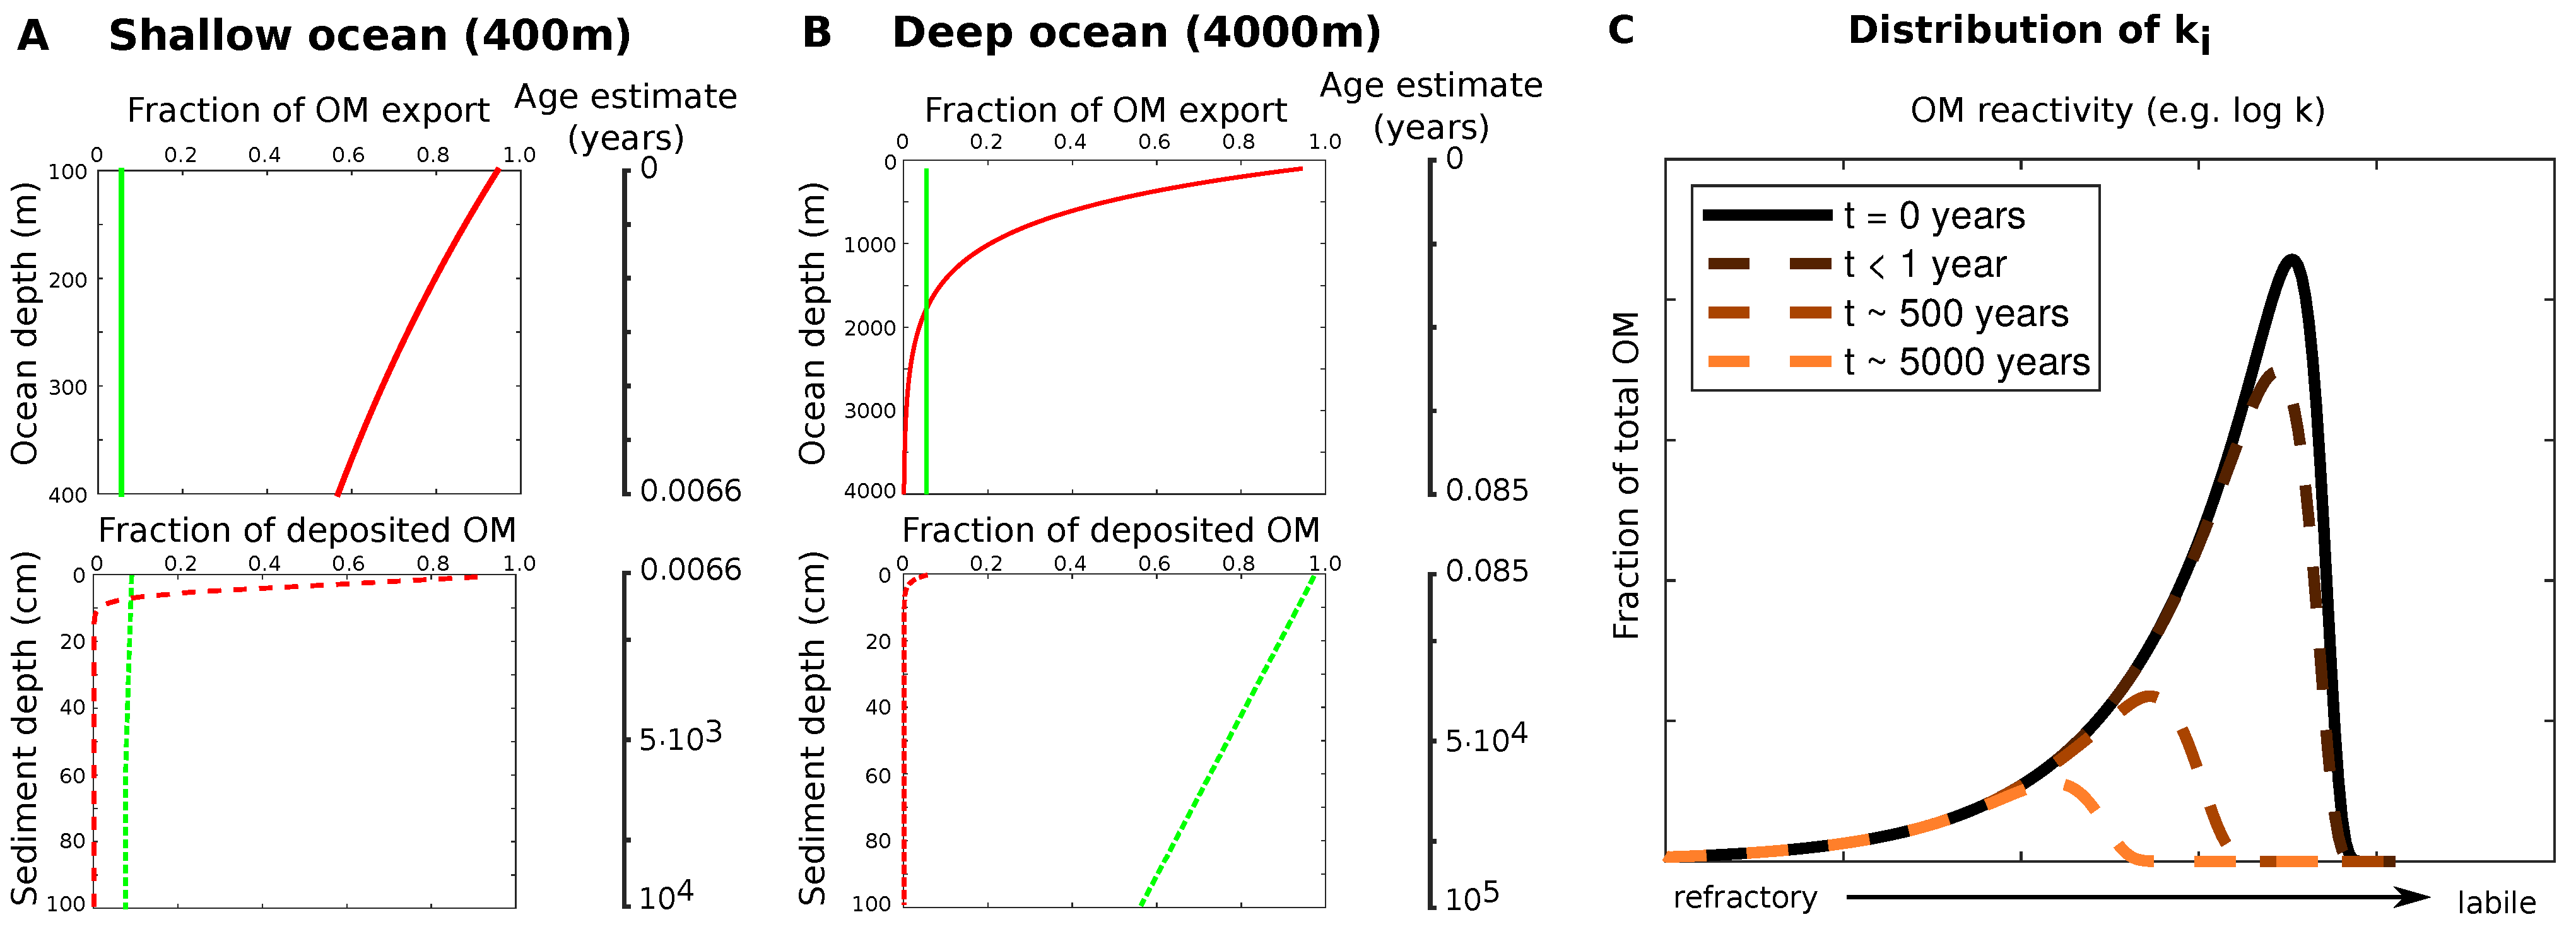
\includegraphics[width=0.9\textwidth]{figures/OM_reactivity/OM_degradation_0808_updated.pdf}
	\caption{Idealised relationship of organic matter decomposition during remineralisation in the water column and the sediments. 
	\textbf{A+B - Upper panels:} Water column development of the two organic matter fractions as represented in cGENIE for two ocean depths 
	(red: labile OM with degradation length scale of 589m; green: refractory OM which is unreactive in the water column). The values are normalised to OM export at 100m. 
	Age estimates for the OM since its export from the euphotic zone are calculated using a sinking velocity of 125m/day. 
	\textbf{A+B - Lower panels:} Schematic representation of the development of the two OM fractions in the sediments (normalised to OM deposited on the seafloor). 
	For the age estimates in the sediment column an advection rate of 0.01 and 0.001cm/yr is assumed, respectively. 
	\textbf{C:} Idealised distribution functions of OM reactive types during remineralisation for different OM ages   
	assuming a reactive continuum model for OM degradation. The initial distribution (at $t=0$) represents fresh OM when it is exported from the euphotic zone 
	\citep[characterised by $a=3e^{-4}$ yr$^{-1}$ and $\nu=0.125$][]{boudreau_comment_2008}.
% \citep[characterised by an average lifetime of the more reactive components a=$3e^{-4}$ yr$^{-1}$ and the dimensionless shape parameter $\nu=0.125$][]{boudreau_comment_2008}, 	
	}\label{fig:OM_reactivity}
\end{center}
\end{figure}

As shown in our sensitivity analysis (Section \ref{subsec:SA}) and discussed by \citet{arndt_quantifying_2013} the 
degradation rate constants for OM ($k_i$) are the most influential parameters and strongly determine the SWI-flux of redox-sensitive elements as well as the preservation of organic matter. 
Yet, their spatial variability is unknown at the global scale and reported rate constants in the sediments can vary by about 10 orders of magnitude or more \citep{middelburg_organic_1993, arndt_quantifying_2013}. 
Furthermore, when OMEN-SED is coupled to cGENIE very different timescales have to be considered for OM degradation in the sediments compared to the water column (Fig. \ref{fig:OM_reactivity}A+B), 
thus rate constants cannot be easily adapted from cGENIE. 
Also, microbes tend to degrade the more reactive organic matter compounds first \citep{emerson_processes_1988, wakeham_compositions_1997, lee_composition_2000}, thus depending on the age of OM (or depth in the sediment and water column) the 
reactivity distribution of its compounds changes significantly (Fig. \ref{fig:OM_reactivity}). 
For instance, in the water column, represented by the reactivity distribution $t<1$ year, only the most reactive OM compounds are 
remineralised. This explains why the POC flux in the ocean can be represented with a 1G or pseudo 2G degradation model. In the sediments much longer timescales have to be considered, 
thus also more reactive compounds are degraded and the reactivity distribution changes significantly already in the upper mm of the sediments ($t \sim 10$ years, Fig. \ref{fig:OM_reactivity}C). 
Therefore, a broader range of OM reactive types must be represented by the degradation model to capture the reactivity spectrum of OM in surface sediments, explaining why at least a pseudo 3G model is required 
\citep[including two degradable and one refractory fraction][]{soetaert_model_1996, boudreau1997diagenetic, stolpovsky_toward_2015}. 
In addition, the advection rate in the sediments determines the age of OM at a specific sediment depth and thus its reactivity. 
For instance, assuming an advection rate of 0.01 cm/yr for the shallow ocean, OM at 5cm depth is about 500 years old, whereas it is one order of magnitude older for an advection rate of 0.001 cm/year in the deep ocean 
and thus covers a broader range of reactive types (Fig. \ref{fig:OM_reactivity}C).  


Thus defining appropriate OM degradation rate constants is a major challenge and source of uncertainty for diagenetic models. The rate constants in models are either determined through profile fitting for a specific site or, 
for global applications, they are related to a single, readily available characteristic (or master variable) of the local environmental conditions. 
For instance, considerable effort has been expended to relate the apparent rate constant for oxic and 
anoxic OM degradation to sedimentation rate ($w$) and various empirical relations have been proposed \citep{toth_organic_1977, tromp_global_1995, boudreau1997diagenetic, stolpovsky_toward_2015}. 
Nevertheless, these relationships are generally based on limited data sets and their global applicability is questionable \citep{arndt_quantifying_2013}. 



\subsubsection{Methodology}
%OMEN-SED is coupled to the global Earth system model cGENIE as described in Section \ref{subsubsec:Methods_ESM_coupling}. 
Our objective is not to perform and discuss a detailed calibration of the two models, as this is beyond the scope of this sediment model development paper. We rather want to showcase, that a coupling is
possible and that the results show main sediment features one would expect to see on a global scale. 
Section \ref{subsubsec:couplingresultscrossplots} compares modelled mean POC weight percentages (wt\%) in the upper 5cm of the sediments to the global distribution pattern of POC content in surface sediments 
(< 5cm sediment depth) of \citet{seiter_organic_2004} using different parameterisations for the degradation rate constants $k_1$ and $k_2$. 
Therefore, the original POC distribution pattern in $1^\circ \times 1^\circ$ grid resolution \citep[interpolated from > 5500 measurements, compare][]{seiter_organic_2004} has been transformed onto the $72\times 72$ SEDGEM grid 
(Figure \ref{fig:TOC_Obs_regridded}). The regridding of the original POC distribution obviously affects the resolution of the data, especially for the continental margin, as some sites with higher POC wt\% are lost due to the 
restricted SEDGEM grid-resolution (compare e.g. maximum values for the East Pacific and upwelling waters of the Namibian shelf, Figure \ref{fig:TOC_Obs_regridded}A + B). 
The colour of the points in Figures \ref{fig:OMEN_GENIE_Boudreau_results} - \ref{fig:OMEN_GENIE_invariant_and_Boudreau} represents SFD of the respective cGENIE grid-cell. As the individual data-points are highly scattered and 
in order to see if a certain relation between $k_1$ and $k_2$ performs better for specific ocean depths, the data-points are binned into 6 uniform depth-classes of 1000m each (respective mean POC wt\% and SFD are represented by 
the triangles). The regression line (and the corresponding R$^2$-value) is calculated for the 6 bin-classes and included in the figures.

\begin{figure}[htbp]
\begin{center}
	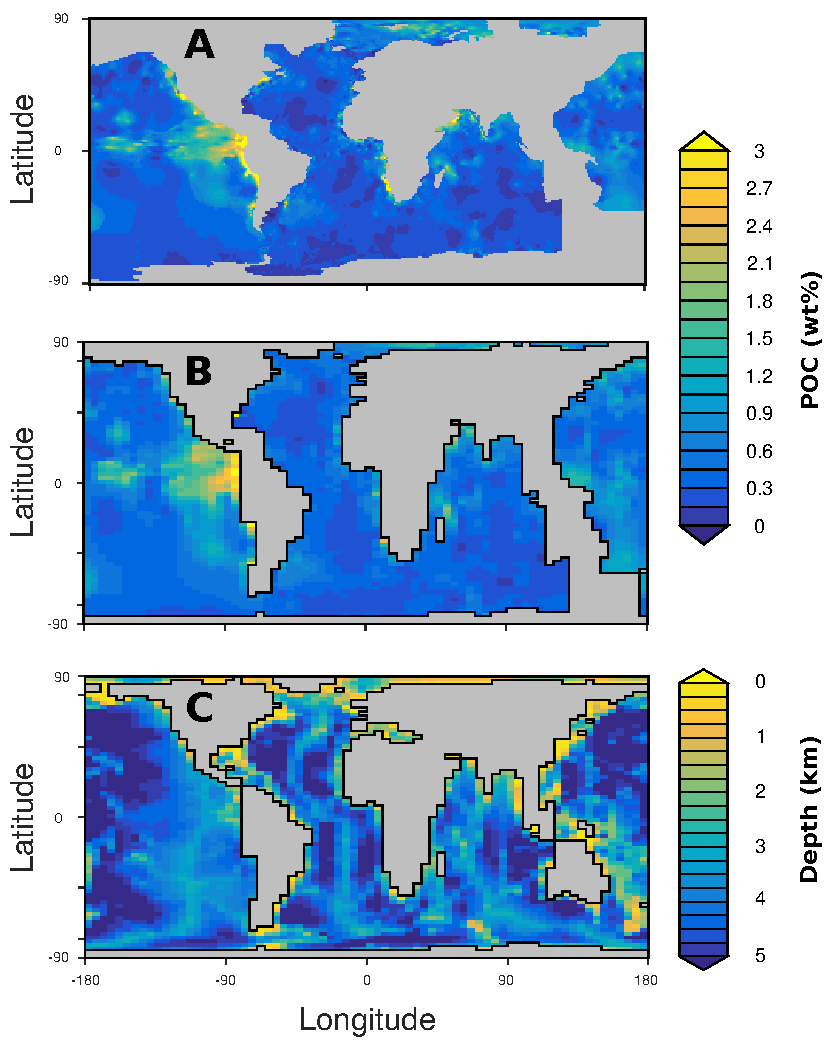
\includegraphics[width=0.8\textwidth]{figures/OMEN-GENIE-Exp/Seiter_interpol_TOCwtpc_compare_until3+GENIEgrid.pdf}
	\caption{Observed distribution of sediment surface (< 5cm) POC wt\% (A, B) and cGENIE bathymetry (C). 
	(A) Original global distribution of POC wt\% interpolated on a $1^\circ \times 1^\circ$ grid from more than 5500 individual data points 
	\citep[compare][for the interpolation procedure]{seiter_organic_2004}. 
	(B) Observed POC wt\% data transformed onto the $72\times 72$ SEDGEM grid. Grid points without any observations are left blank (grey). 
	(C) Gridded continental configuration and ocean bathymetry of the 16-level, $72\times 72$ equal-area cGENIE grid.
	}\label{fig:TOC_Obs_regridded}
\end{center}
\end{figure}

\textcolor{red}{TODO Andy: Section describing the prescribed fields of solids (i.e. detrital, opal, \chem{CaCO_3}) to the sediments!}

To parameterise the reactivity of organic matter in OMEN-SED two different approaches are compared. First, globally invariant degradation rate constants $k_1$ and $k_2$ are assumed. 
By providing two pools of POC from the water-column characterised by different degradation rate constants, cGENIE accounts for the decrease in mean POC reactivity with water-depth. 
The rate constants for the more refractory OM pool, $k_2$, is systematically varied between 0.004 and 0.006 year$^{-1}$ and the more labile OM component, described by $k_1$, is assumed to degrade $x \in \{1.1, 1.2, 1.3, 1.5, 2\}$ times faster, respectively. 
However, although accounting for the decrease in mean POC reactivity with seafloor depth, this approach does not take into account the change in organic matter reactivity types caused by different burial velocities and thus time scales in the sediments 
(Fig. \ref{fig:OM_reactivity}). 
Therefore, the second approach uses the empirical relationship proposed by \citet{boudreau1997diagenetic}, 
which relates the apparent OM degradation rate constant in the upper sediments to the burial velocity, $w$ (cm year$^{-1}$, see also Section \ref{subsec:globalhypsometry}):
\begin{equation}
 k_\mathrm{app} = 0.38 \cdot w^{0.59}.
\end{equation}
Following \citet{boudreau1997diagenetic} and \citet{stolpovsky_toward_2015} it can be assumed that $k_\mathrm{app}$ represents the mean OM reactivity within the upper 10-20cm of the sediments. 
The following assumptions are made in order to calculate the two degradation rate constants for OMEN-SED:
\begin{align}
  k_\mathrm{app} &= f_1 \cdot k_1 + f_2 \cdot k_2 \label{boudreau_assumption1}\\
  k_1 &= x \cdot k_2					\label{boudreau_assumption2}
\end{align}
where $x$ describes the relation between $k_1$ and $k_2$ and is subject to sensitivity experiments (with values of $x \in \{2, 5, 8, 10, 12, 15, 20, 25\}$). 
As the fractions of labile and refractory OM reaching the sediments ($f_1, f_2$) is known from cGENIE, $k_1$ and $k_2$ can be calculaed independently for each grid-cell. 
All simulations presented here are run for 10,000 years to steady-state from a 20,000 year cGENIE spin-up without OMEN-SED. The new model OMEN-SED is called for each grid-cell in every time step, feeding back the resulting SWI-fluxes and the 
fraction of POC preserved in the sediments to cGENIE. 

\subsubsection{Results}\label{subsubsec:couplingresultscrossplots}
\begin{figure}[htbp]
\begin{center}
	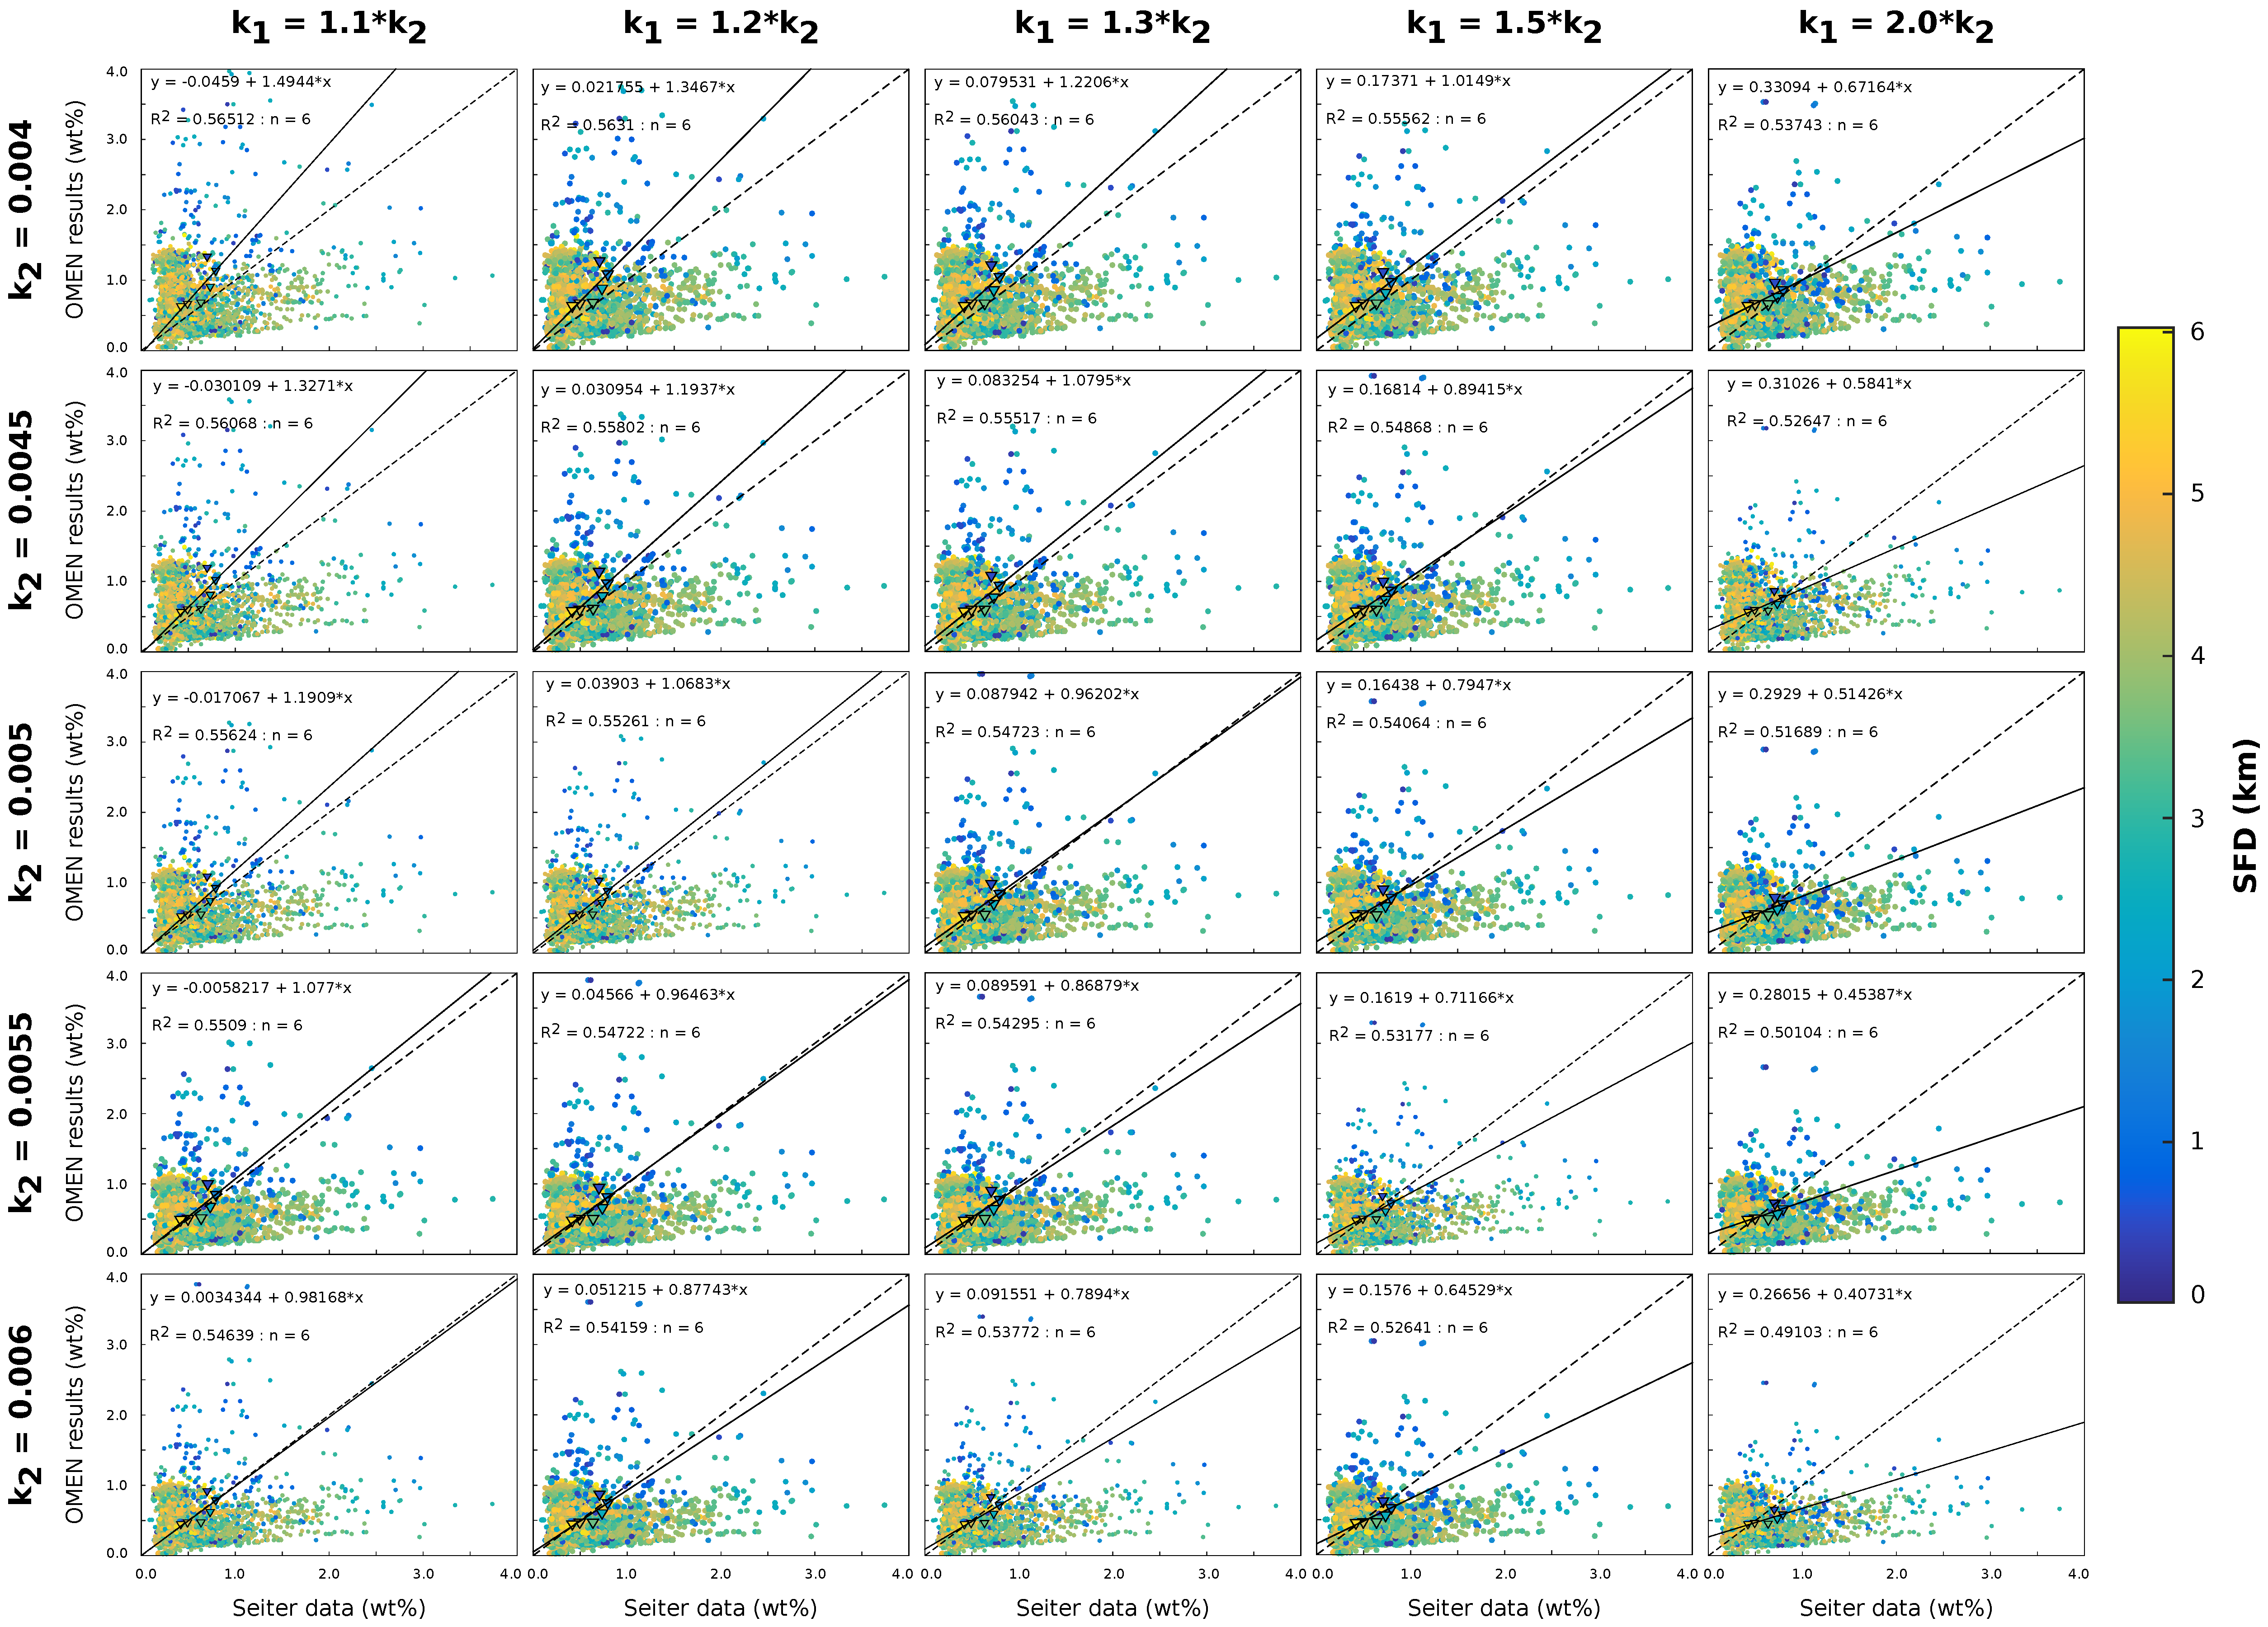
\includegraphics[width=1.0\textwidth]{figures/OMEN-GENIE-Exp/0_2908_Invariant_k_CROSSPLOT_WITH_REGRESSION.pdf}
	\caption{Crossplots comparing modelled and observed mean POC wt\% in the upper 5 cm of the sediments using globally invariant degradation rate constants $k_1$ and $k_2$. 
	Data-points are binned into 6 uniform depth-classes of 1000m as in Fig. \ref{fig:OMEN_GENIE_Boudreau_results}, each class is represented by a triangle. 
	Grid-points with more than 4.0 POC wt\% are not shown.}\label{fig:OMEN_GENIE_invariant_results}
\end{center}
\end{figure}
% However, imposing the depth dependent relation of the degradation rate constants is rather arbitrary and the POC wt\% data used for the comparison has their own limitations (compare Section\ref{subsec:Parameterising_OM_rate_const}). 
% In addition, the empirical relationship used \citep{boudreau1997diagenetic} and the regression model obtained is based on modern day observations and very likely not valid under different environmental conditions during Earth 
% history \citep[e.g.][]{hulse_understanding_2017}.
%First, the degradation rate constants are parameterised on model intrinsic information only using the globally invariant approach. By providing two pools of POC from the water-column characterised by different degradation rate constants, cGENIE accounts 
%for the decrease in bulk POC degradability with water-depth. 
%Therefore, the imposed depth dependent relation of the degradation rate constants presented in Figure \ref{fig:OMEN_GENIE_Boudreau_results} could also be regarded as double-accounting. 
Figure \ref{fig:OMEN_GENIE_invariant_results} presents results for the globally invariant degradation rate experiments. 
%, where $k_2$ is systematically varied between 0.004 and 0.006 year$^{-1}$ and the more labile OM component, $k_1$, is assumed to degrade $x \in \{2, 3, 4, 5, 10\}$ times faster, respectively. 
In general, using globally invariant degradation rate constants 5 of the 6 bin-classes are located closer to the 1:1 line as in the experiments using the \citet{boudreau1997diagenetic} relation (Fig. \ref{fig:OMEN_GENIE_Boudreau_results}). 
Also the slope of some regression lines is close to 1.0 
(e.g. $(k_2, x) \in \{ (0.004, 1.5),  (0.0045, 1.3), (0.005, 1.2), (0.005, 1.3), (0.0055, 1.1), (0.0055, 1.2), (0.006, 1.1)\}$), indicating that the simpler parameterisation captures the rate of change in modeled and observed POC wt\% for the bin-classes 
rather well. 
The shallowest bin-class (between 0 and 1000m) represents an exception, as OMEN-SED tends to overestimate POC preservation for this depth class. However, this could also be related to the regridding of the original POC distribution 
pattern of \citep{seiter_organic_2004} on to the SEDGEM grid, as some data grid-cells with higher POC wt\% on the continental margin are lost due to the restricted SEDGEM resolution (compare Section \ref{subsec:Parameterising_OM_rate_const}). 
Overall, using this parameterisation a relationship where the labile POC fraction degrades not more than 1.5 times faster than the refractory fraction fits the 
\citet{seiter_organic_2004} data better than a larger spread between both POC pools (i.e. $x > 2.0$). 
\textcolor{red}{Say something about, that this can potentially be explained as the observations represent OM concentrations in the upper 5cm of the sediments where the range of reactivities to be considered is smaller than 
deeper down in the sediments... Fig. \ref{fig:OM_reactivity}??? Therefore, degradation rate constants are not very different.}
%This can potentially be explained as the observations represent organic matter concentrations in the upper 5cm of the sediments 


\begin{figure}[htbp]
\begin{center}
	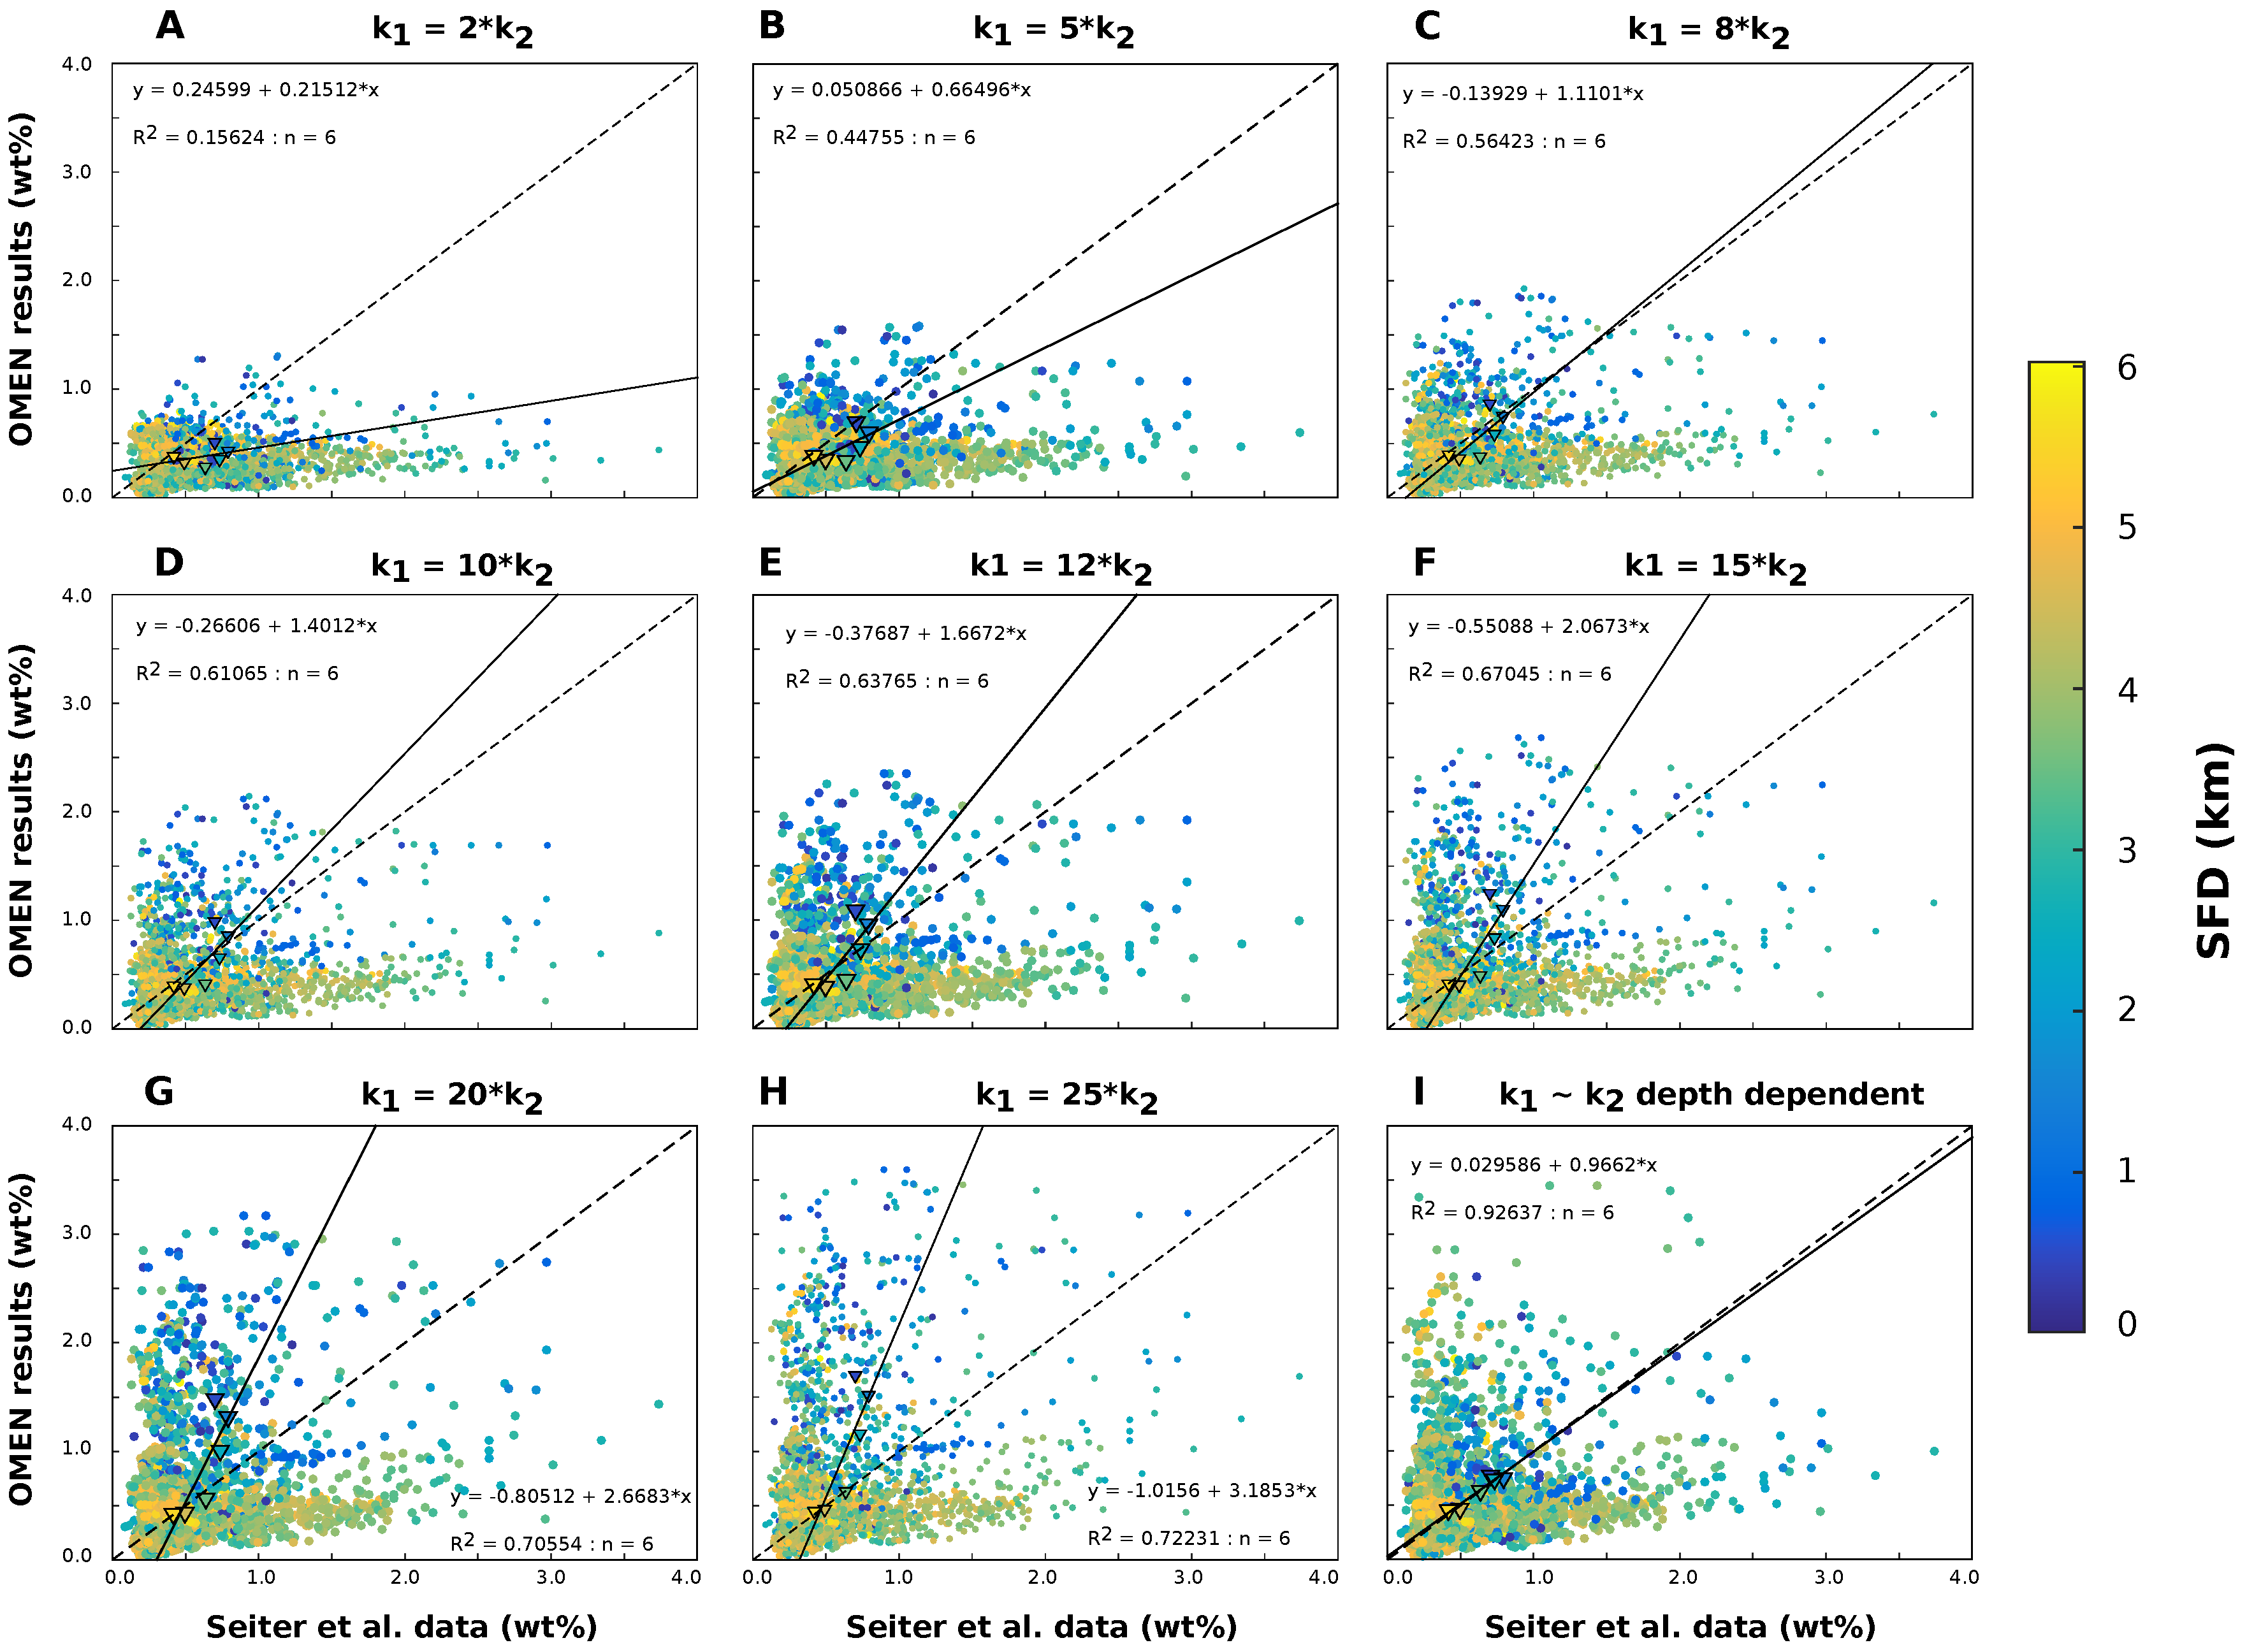
\includegraphics[width=1.0\textwidth]{figures/OMEN-GENIE-Exp/0_Boudreau_CROSSPLOTS_290817.pdf}
	\caption{Crossplots comparing modelled and observed mean POC wt\% in the upper 5 cm of the sediments using the relationship of \citet{boudreau1997diagenetic} and the assumptions of Eq. (\ref{boudreau_assumption1}) and 
	(\ref{boudreau_assumption2}) to calculate $k_1$ and $k_2$.  Data-points are binned into 6 uniform depth-classes of 1000m, each class is represented by a triangle. 
	Grid-points with more than 4.0 POC wt\% are not shown.}
	\label{fig:OMEN_GENIE_Boudreau_results}
\end{center}
\end{figure}


Next the relationship of \citet{boudreau1997diagenetic} and the assumptions of Eq. (\ref{boudreau_assumption1}) and (\ref{boudreau_assumption2}) are used to calculate $k_1$ 
and $k_2$. In Figure \ref{fig:OMEN_GENIE_Boudreau_results} (A-H) the relation between the two degradation rate constants (Eq. (\ref{boudreau_assumption2})) is changed globally, thus independent of the seafloor depth. 
The crossplots show that it is not possible to achieve a solution where all bin-classes fall onto, or close to, the 1:1 line. Also, the slope of the regression lines are generally much larger or smaller than 1.0 
(with the exception of Figure \ref{fig:OMEN_GENIE_Boudreau_results}C), indicating that the rate of change in modeled and observed POC wt\% for the bin-classes is different. 
The R$^2$ values are strictly monotonically increasing for increasing $x$ because a depth-dependency is artificially imposed for the modelled POC wt\% through the relation between $k_1$ and $k_2$. 
When looking at the individual bin-classes it can be seen that shallow ocean depths are better represented by smaller differences between $k_1$ and $k_2$ (e.g. $k_1 = 5 \cdot k_2$ for SFD < 1000m, Figure \ref{fig:OMEN_GENIE_Boudreau_results}B),
and the deep ocean by a larger spread (e.g. $k_1 = 25 \cdot k_2$ for SFD > 3000m, Figure \ref{fig:OMEN_GENIE_Boudreau_results}H). 
These results reflect the preferential degradation of more reactive organic matter types \citep{wakeham_compositions_1997, lee_composition_2000} and thus the change in the distribution functions of OM reactive types for different OM ages (Fig. \ref{fig:OM_reactivity}C). 
In the shallow ocean bulk POC consists of fresher organic matter types and is therefore generally more reactive (i.e. higher $k_\mathrm{app}$ due to higher $w$ in the model) as in the deep ocean. In addition, OM at 5cm sediment depth in the deep ocean 
is generally older as in the shallow ocean due to lower advection rates, therefore more reactive types are affected by degradation and a larger spread between k-values is needed to capture these dynamics (compare Fig. \ref{fig:OM_reactivity}C). 
% In a greatly simplified way, this can be interpreted as bulk POC in the shallow ocean being more reactive (i.e. higher $k_\mathrm{app}$) and consisting of fresher organic matter types, therefore the degradation rate constants of the 
% two pools are more similar (i.e. $k_2 < k_1$). In the deeper ocean, bulk POC is generally less reactive (i.e. lower $k_\mathrm{app}$) and due to the preferential degradation of more reactive organic matter types in the water-column 
% \citep{wakeham_compositions_1997, lee_composition_2000} the refractory POC pool can be considered as being several orders of magnitude less reactive compared to the labile POC pool (i.e. $k_2 \ll k_1$). 
We use these observations to create a depth dependent relationship between the two degradation rate constants, where $x$ in Eq. (\ref{boudreau_assumption2}) takes values of $x=5$ for SFD < 1000m, $x=8$ for 1000m $\leq$ SFD < 2000m, 
$x=12$ for 2000m $\leq$ SFD < 3000m and $x=25$ for SFD $\geq$ 3000m for the 6 SFD bin-classes, respectively. 
In this depth dependent model all bin-classes are close to the 1:1 line and the resulting regression model accounts for 92.6\% of the variance of the modeled POC wt\% around the observed mean of the bin-classes (Figure \ref{fig:OMEN_GENIE_Boudreau_results}I). 
Furthermore, the slope of the regression line (0.9662) indicates that the rate of change in modeled and observed POC wt\% for the bin-classes is comparable.
%>>>
\marginnote{\textbf{DH}: more statistics, e.g. p-value don't make much sense right?}[-1cm]%<<<




\begin{figure}[htbp]
\begin{center}
	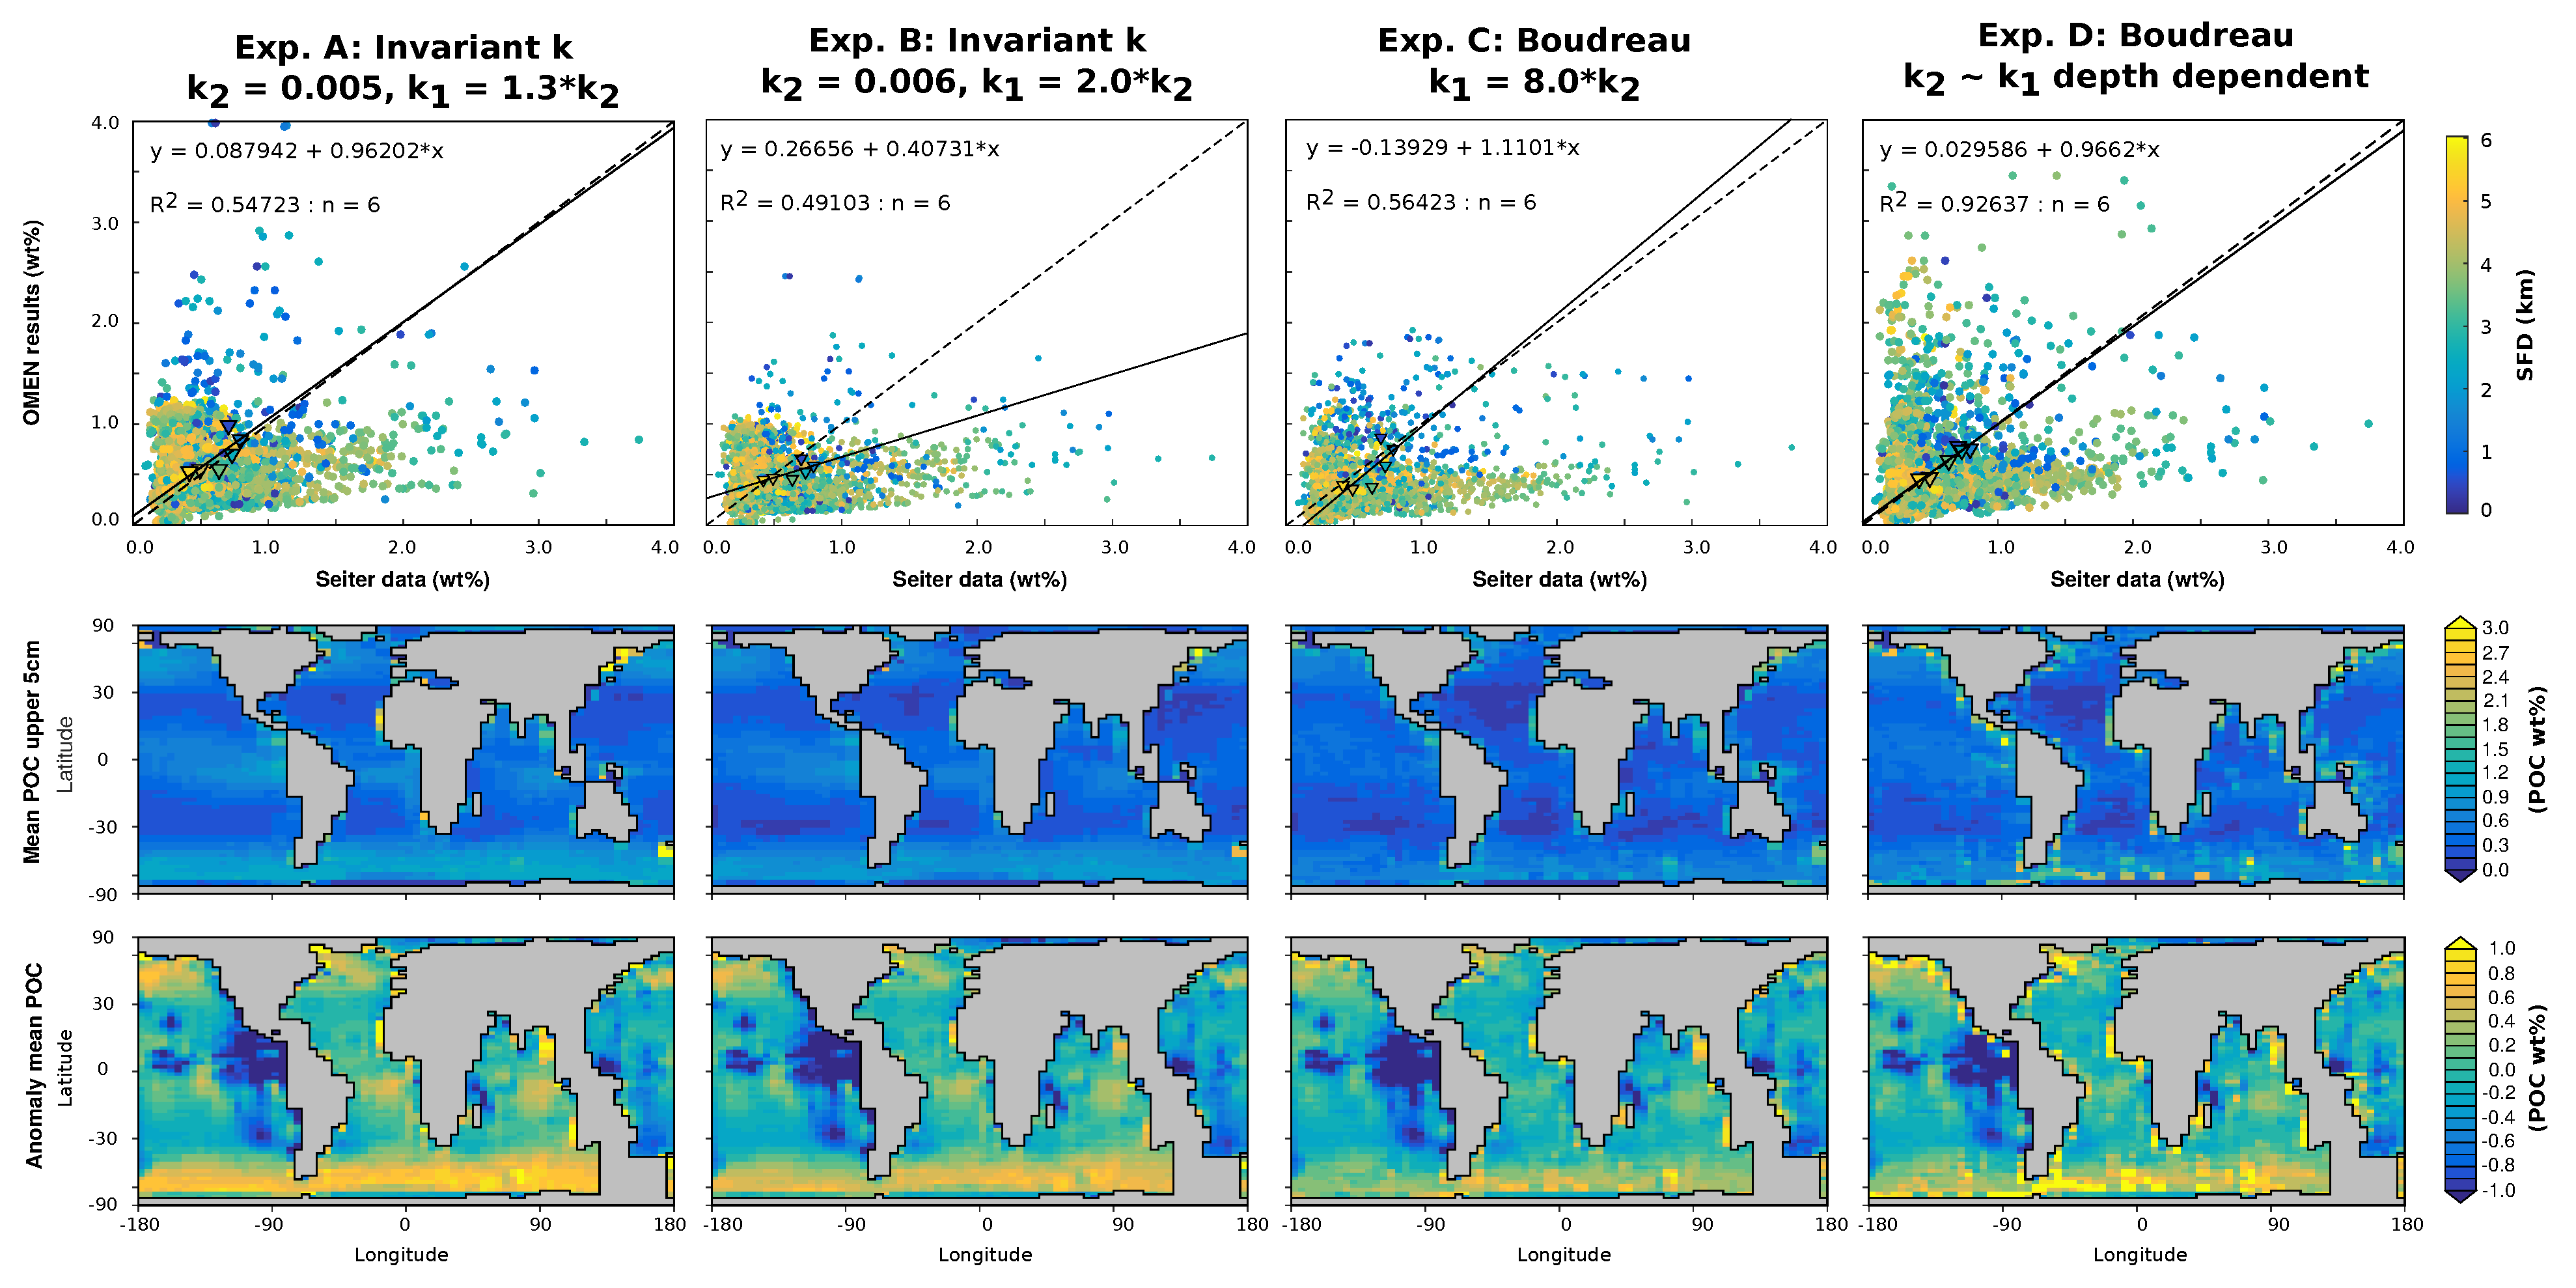
\includegraphics[width=1.0\textwidth]{figures/OMEN-GENIE-Exp/0_2908_COMPARE_INVARIANT_BOUDREAU_POC.pdf}
%	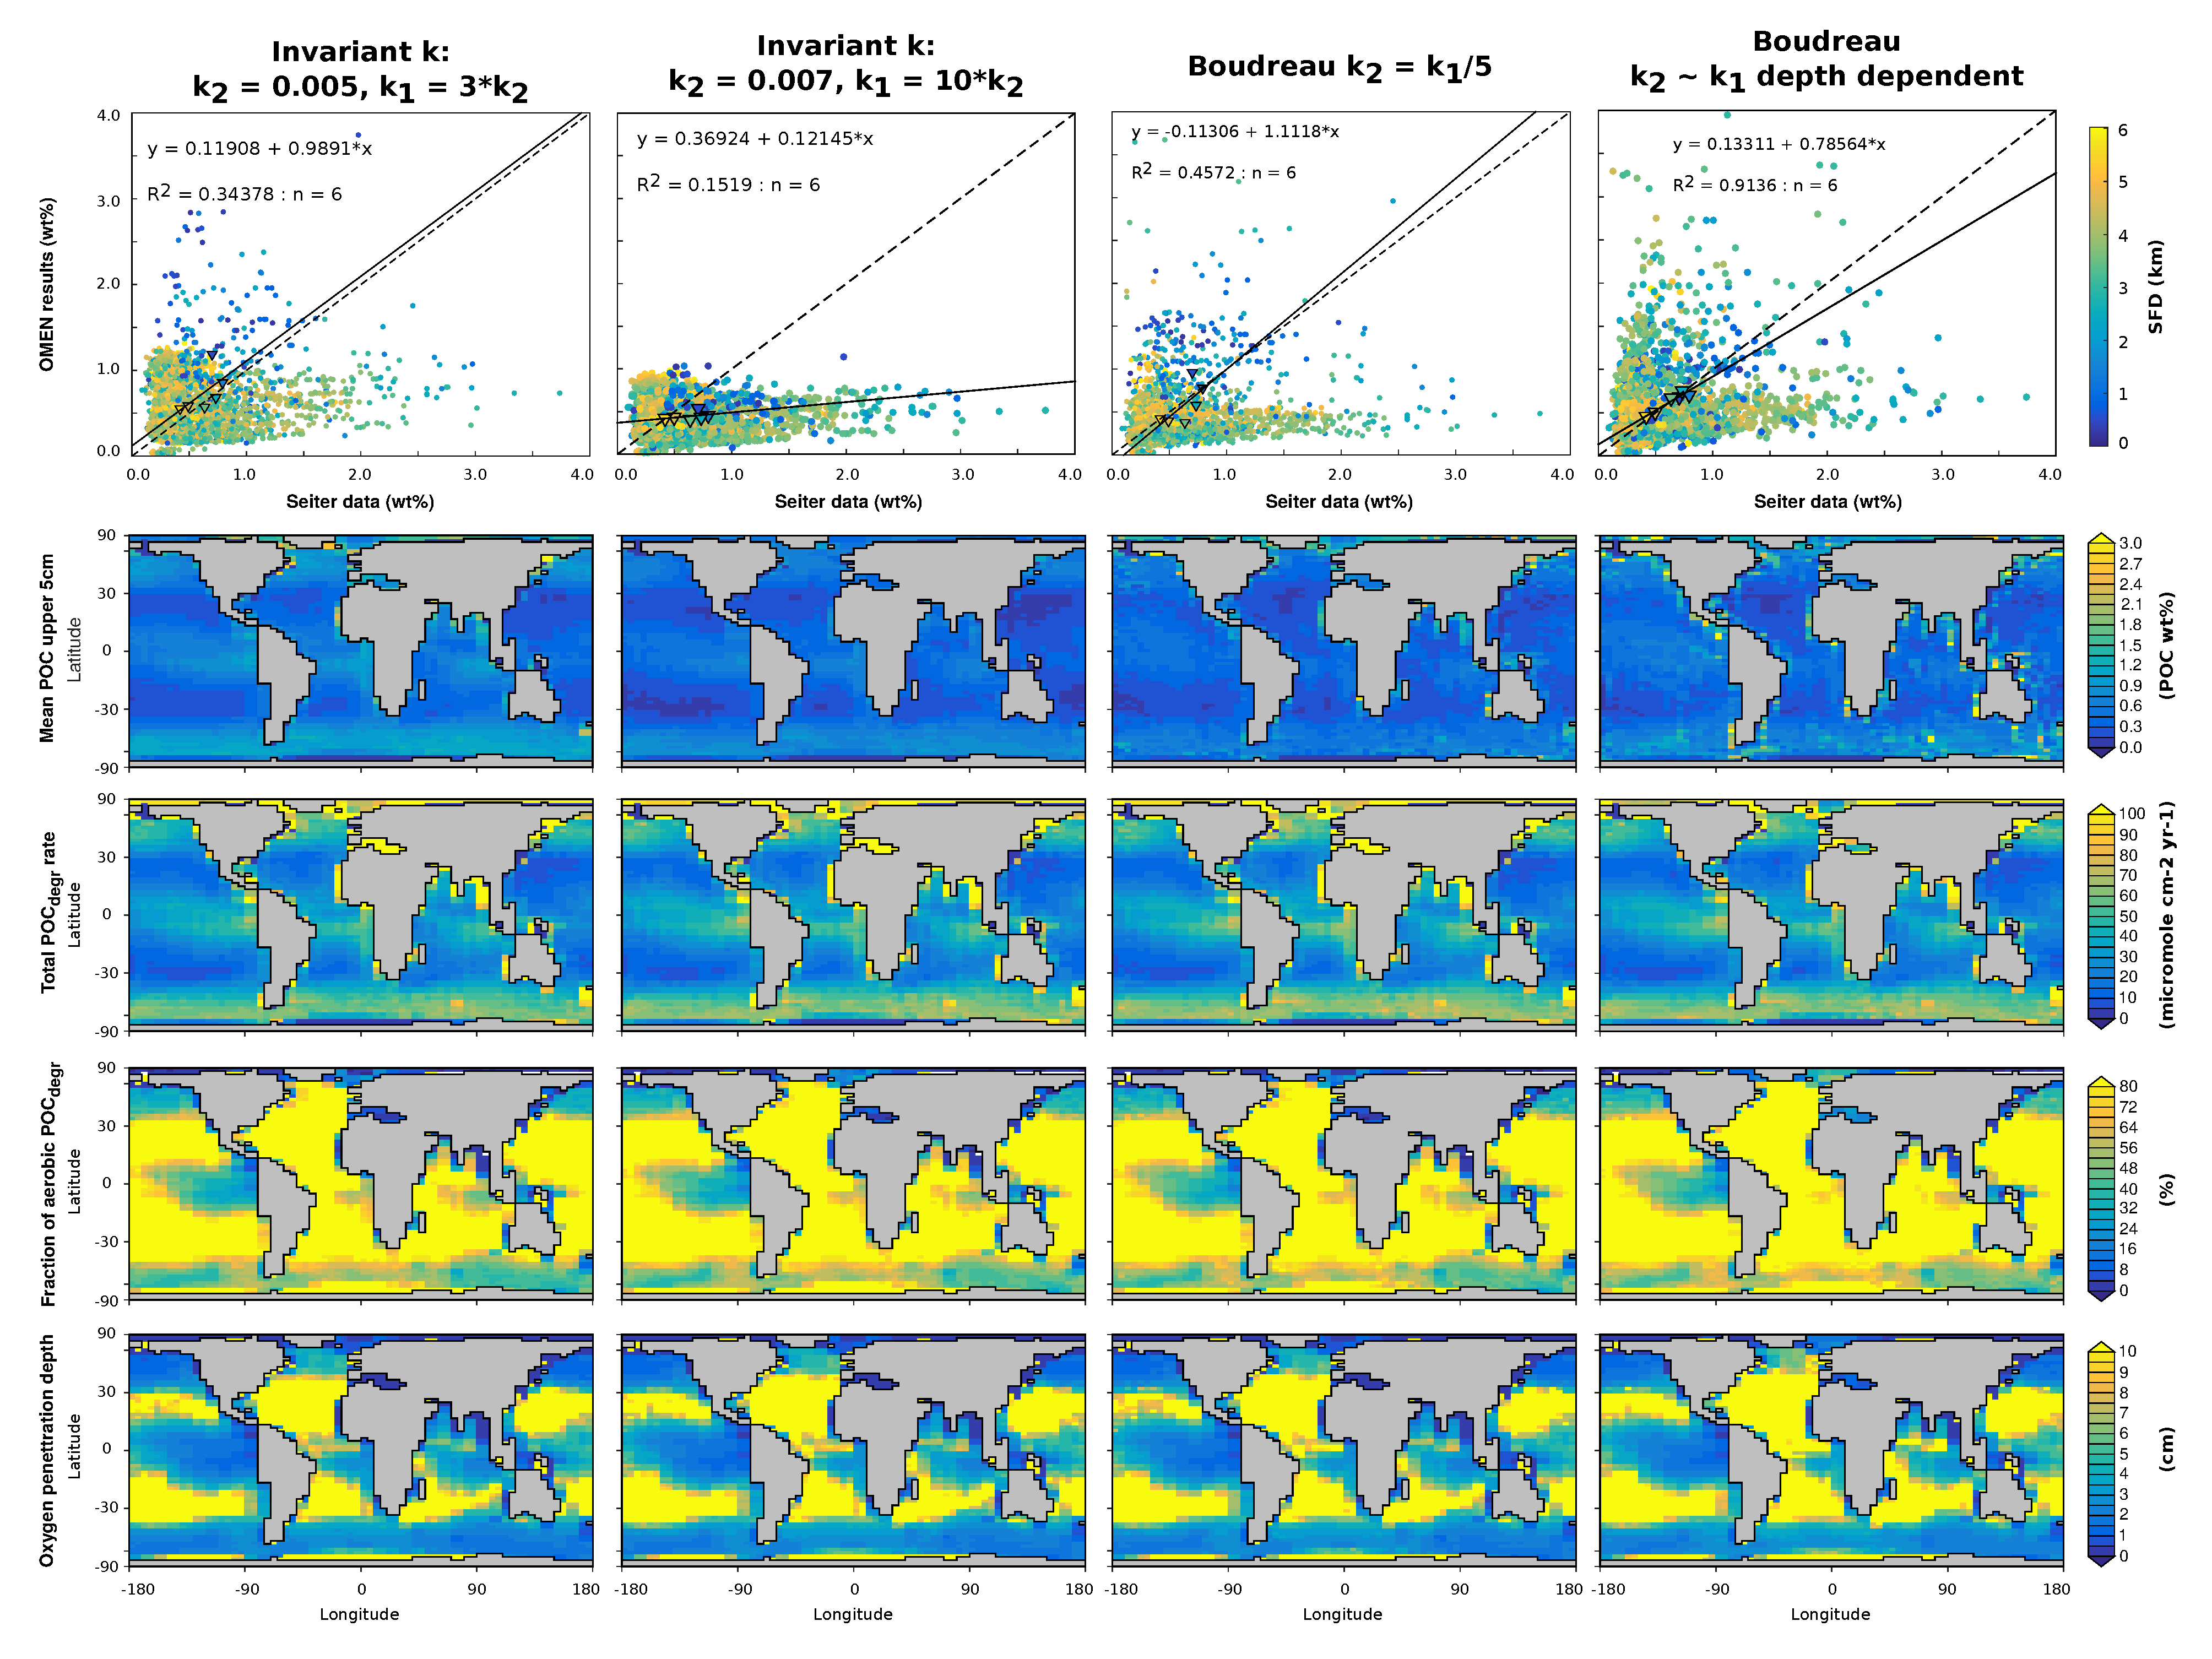
\includegraphics[width=1.0\textwidth]{figures/OMEN-GENIE-Exp/0_1507_1707_COMPARE_INVARIANT_BOUDREAU_noANOMALY.pdf}
	\caption{Mean POC concentrations in the upper 5cm of the sediments (\chem{POC_{5cm}}) from the coupled OMEN-cGENIE model using representative parameterisations \citep[invariant and after][]{boudreau1997diagenetic} 
	for the OM degradation rate constants ($k_1$, $k_2$, compare Section \ref{subsec:Parameterising_OM_rate_const}). 
	1st row: Crossplots as shown in Fig. \ref{fig:OMEN_GENIE_Boudreau_results} and \ref{fig:OMEN_GENIE_invariant_results}. 
	2nd row: \chem{POC_{5cm}} as calculated with OMEN-SED. 
	3rd row: Difference map of \chem{POC_{5cm}} as calculated with OMEN-SED and interpolated data from \citet{seiter_organic_2004}.
	}\label{fig:OMEN_GENIE_invariant_and_Boudreau}
\end{center}
\end{figure}

\textcolor{red}{DH: include Fig. \ref{fig:OMEN_GENIE_invariant_and_Boudreau}? As not much difference \& do we learn anything?} 
Figure \ref{fig:OMEN_GENIE_invariant_and_Boudreau} compares mean POC concentrations in the upper 5cm of the sediments (\chem{POC_{5cm}}) from two 
globally invariant degradation rate constant approaches (experiments A and B, i.e. $(k_2, x) \in \{(0.005, 1.3), (0.006, 2.0)\}$) 
with two approaches using the relation of \citet{boudreau1997diagenetic} (experiments C and D, with $k_1 = 8 \times k_2$ and the depth dependent parameterisation). 
Within the globally invariant approaches of Figure \ref{fig:OMEN_GENIE_invariant_results} the depth bin-classes for experiment A fall closest to the 
1:1 line whereas experiment B is the parameterisation with the smallest POC preservation. 
%\textcolor{red}{Maybe use $(k_2, x) = (0.0045, 2)$ instead of $(k_2, x) = (0.007, 10)$, as we hopefully see more OM preservation and larger differences in Fig. \ref{fig:OMEN_GENIE_invariant_and_Boudreau}}
%Global difference maps of model and observed surface sediment POC wt\% are compared and 
%Even though the crossplots show different results, the global patterns are very similar across experiments (Fig. \ref{fig:OMEN_GENIE_invariant_and_Boudreau}). 
All 4 experiments reproduce minimal POC concentrations in the subtropical gyres and generally higher concentrations along the continental margins (Fig. \ref{fig:OMEN_GENIE_invariant_and_Boudreau}, 2nd row). 
All experiments, however, underestimate mean POC wt\% in the surface sediments of the equatorial east Pacific and overestimate POC concentrations 
in the North Pacific and Southern Oceans, especially experiment A and D (Fig. \ref{fig:OMEN_GENIE_invariant_and_Boudreau}, 3rd row). 
The depth dependent approach of \citet{boudreau1997diagenetic} shows more spatial variability in POC preservation than the other parameterisations. 
In general, implementing lower, anaerobic degradation rate constants when bottom water oxygen concentrations fall below a threshold value could potentially improve the simulation of higher POC concentrations in areas with high POC input to the 
sediments \citep{palastanga_long_term_2011}. 
 

\subsection{Modelled fluxes and sediment characteristics}
For the globally invariant experiment A ($(k_2, x) = (0.005, 1.3)$) modelled SWI-fluxes and sediment characteristics are shown in Figure \ref{fig:OMEN_GENIE_best_fit_invariant}.
Modelled total POC degradation (\chem{POC_{degr}}) rates in the upper sediments decrease from the shelves to the deep sea by up to 2 orders of magnitude (Fig. \ref{fig:OMEN_GENIE_best_fit_invariant}B). 
This is in agreement with data from the literature \citep[e.g.][]{middelburg_organic_1993, middelburg_empirical_1997} and other model results 
\citep[e.g.][]{thullner_global_scale_2009} which indicate that the highest degradation rates in marine sediments are found in the coastal ocean (SFD < 200m). 
Oxygen fluxes into the sediments (Fig. \ref{fig:OMEN_GENIE_best_fit_invariant}C) range from 0.0 for the deep ocean and sites without OM deposition until 269.55 $\mu$mol cm$^{-2}$yr$^{-1}$ for the shallow ocean with the highest POC degradation rates. 
Influx of \chem{SO_4}  into the sediments is rather low (between 0.0 and 23.9 $\mu$mol cm$^{-2}$yr$^{-1}$) because in OMEN-SED 95\% of produced \chem{H_2S} is reoxidised to \chem{SO_4}, therefore sulfate reduction is mainly driven by in situ sulfide oxidation. 
However, in general the coupled model fluxes fall well within the range predicted by the stand-alone global hypsometry experiments (Section \ref{subsec:globalhypsometry}). 
In accordance with the total POC degradation rates the release of \chem{PO_4} shows a maximum value of 7.62 nanomol cm$^{-2}$yr$^{-1}$ at the shelves (Fig. \ref{fig:OMEN_GENIE_best_fit_invariant}D). 
The relative contribution of aerobic POC degradation in the upper sediments increases from the shelves to the deep sea (Fig. \ref{fig:OMEN_GENIE_best_fit_invariant}G) 
which is also consistent with estimates from %the literature \citep[e.g.][]{middelburg_empirical_1997} as well as other model results. 
\citet{thullner_global_scale_2009} who found that oxygen is responsible for less than 10\% of \chem{POC_{degr}} at 100m SFD and for more 
than 80\% in the deep sea. 
The oxygen penetration depth in OMEN-SED increases from below 1cm at the shelves to more than 10cm in the deep ocean (Fig. \ref{fig:OMEN_GENIE_best_fit_invariant}H).
Small oxygen penetration depths of a few millimetres are typical for bioturbated sediments at the coastal ocean \citep[e.g.][]{wenzhofer_benthic_2002} and 
the oxygen penetration depth has been shown to increase exponentially with SFD to more than 10cm in the deep sea \citep{glud_oxygen_2008}. 



\begin{figure}[htbp]
\begin{center}
	\includegraphics[width=1.0\textwidth]{figures/OMEN-GENIE-Exp/0_2908_INVARIANT_SED_PROPS_AND_FLUXES_0808_LINES.pdf}
	\caption{Sediment characteristics related to POC degradation and oxygen consumption for the globally invariant paramaterisation with $k_2= 0.005,\ k_1 = 1.3 \cdot k_2$ (Exp. A).
	Total \chem{POC_{degr}} rate and fraction of aerobic \chem{POC_{degr}} are the respective values for the first 5cm in the sediments. 
	%Results of OMEN-cGENIE coupling using the OM degradation rate constants which produce the best fit to the \citet{seiter_organic_2004} 	observations (i.e. $k_1 = 0.015,\ k_2 = 0.005$). 
	%All results shown are sediment characteristics calculated with OMEN-SED. 
	}\label{fig:OMEN_GENIE_best_fit_invariant}
\end{center}
\end{figure}

% - Total Cox rate: Cox decreases from the shelves to deep-sea: Total Cox rate is $\sim$50 times greater at 100m than at 5000m 
% (Middelburg et al., 93; Thullner et al., 09; Schulz \& Zabel, 05)\\
% 
% - Fraction of aerobic Cox:  O2 gets more important as TEA with increasing SFD: <10\% at shallow SFD vs >80\% in the deep-sea (Thullner et al., 09)\\
% 
% - zox increases from < 1 cm at 100 m; to > 10 cm at 5000m (Glud, 08; Meile \& Van Cappellen, 03)\\
%  Stolpovsky: bioturbated sediments deposited at continental margins quickly become anoxic within a few millimeters [Wenzhöfer and Glud, 2002].



%E.g. Thullner et al. 2009! \\

% Schulz and Zabel: 
% The basic mechanism inducing microbial activity
% is the supply of organic matter to the seafloor and
% this is generally coupled to surface water produc-
% tivity. Most of the highly productive areas in the
% global ocean are adjacent to the continents, so 
% that we can expect a decrease of degradation inten-
% sity from the coastal marine environments over
% the continental shelves and slopes into the deep-
% sea. This becomes evident when we look at the
% data compiled by Middelburg et al. (1993) which
% indicate that 83\% mineralization and 87\% burial in
% marine sediments occurs in the coastal zone
% occupying only ~9\% of the total ocean area. This
% means that the sediments with the highest respi-
% ration rates also have the highest burial efficiency
% in marine environments.
% Fluxes of oxygen and nitrate, therefore, vary
% over several orders of magnitude between oligo-
% trophic open ocean areas and continental shelf and
% slope areas. This is about 50 to 6,000 mmol m -2 yr -1
% for oxygen and -600 to 380 mmol m -2 yr -1 for nitrate ...
% 
% (SHOW O2, NO3 AND E.G. PO4 SWI-fluxes).



% Could also plot Figure 4 from Palastanga et al. (2011) with POC wt\% for different sites in the ocean!
% \textcolor{red}{UNITS of Fe-P! This is a solid! Therefore not nmol/cm3 rather mol/g as in Palastanga... }\\
% 
% Also check what water column features to show and maybe sediment P or Fe-P concentrations (see PALASTANGA et al. 2011, 2013).
% 
% 

% Fe-P supply problem (see Palastanga et al. 2011): ... the sinking flux of atmospheric P is ultimately deposited
% into the sediment. Up-to-date, there is very little data on the speciation of atmospheric P ... we assume an constant aeolian supply of P as Fe-P to the sediments of ....

% From Boudreau book on POC fractions and their degradation constants:
% Furthermore, it has been realized that there is not a single
% organic matter type in sediments, but many. The data suggest that there is a reactive
% fraction, k1, that decays within the top 10-20 cm of sediments, a more refractory
% component, k2, that oxidizes on a scale of about ten to one hundred times longer, and a
% third that is largely inert. The k2 material is largely, if not completely, subject to
% anoxic decomposition. There is also a highly reactive component, say ko, that
% decomposes on a seasonal time scale, largely at the sediment-water interface and in the
% top centimeter of sediments, i.e. ko = 1-10 yr-1. Predictive correlations have, so far,
% been applied only to k1 and k2.

% From Stolpovsky: 
% Our objective was to find an empirical function relating the depth distribution of POC mineralization to rain
% rate (RRPOC). This is an attractive master variable because (i) POC fluxes to the seafloor are reasonably well
% known and routinely computed by ESMs [e.g., Dunne et al., 2007] and (ii) POC reactivity appears to be
% correlated with rain rate [Emerson et al., 1985; Murray and Kuivila, 1990; Soetaert et al., 1996; Boudreau, 1997;
% Martin and Sayles, 2006].
% 
% Middelburg: Ocean margin sediments (<2000 m) account for about 85% of the material
% accumulating in the ocean and about 80-90\% of the mineralization in marine sediments.  


\section{Scope of applicability and model limitations}\label{sec:Appl_Limitations}
\textbf{Dominik: Needs polishing!? This is my first draft}
State-of-the art numerical models representing the full complexity of the diagenetic processes typically perform adequately at reproducing site-specific biogeochemical dynamics, however, tuning model parameters is laborious, 
the computational demand is high and, thus, their transferability to the global scale is limited. On the other hand, analytical models are very efficient, but existing approaches coupled to global models generally use highly 
simplified reaction networks, often restricted to oxic degradation with a limited number of explicit pore water tracers. However, our ability to assess the role of organic matter dynamics for global biogeochemical cycles and climate 
requires tools that resolve the most important biogeochemical processes and tracers explicitly, while at the same time are computationally efficient and have a degree of predictive capability to extrapolate knowledge to data poor areas. 
The new model OMEN-SED presented here is a legitimate compromise between complexity of biogeochemical processes and computational efficiency. 
Its scope of applicability covers the entire range from regional to global scales. 
OMEN-SED's computational efficiency facilitates its use in two very different ways. Firstly, it can be coupled to global Earth system models and therefore allows the investigation of coupled global biogeochemical dynamics over different timescales. 
Secondly, it can be used to calculate quantitative sensitivity indices requiring large sample sizes such as variance- or density-based approaches. Therefore, OMEN-SED can help to quantitatively investigate how systematic variations in model parameters 
impact the model output, for instance when the model has been tuned to a site-specific problem. 
Due to the represented anaerobic processes and secondary-redox reactions, OMEN-SED is also useful to investigate the role of benthic-pelagic coupling on the development of ocean anoxia and euxinia for instance during extreme climate 
events such as OAEs. On more regional scales it can be applied to systems like continental margins or estuaries which are characterised by complex interactions between different pathways of organic matter degradation and redox reactions. 
Here, the model can help to disentangle the complex process interplay that drives the biogeochemical dynamics and give quantifications for upper and lower constraints of carbon and nutrient budgets for these dynamic systems. 
In addition, OMEN-SED can be used to model eutrophication processes in shallow coastal waters as sediment-water oxygen and nutrient exchange fluxes are explicitly modelled and depend on reoxidation of reduced substances which causes 
a substantial part of oxygen consumption in these environments. %diagenetic OM degradation, bottom water concentrations, temperature.  

However, the model presented here, even more complete than previous analytical models, is still associated with a certain degree of simplifications. In order to solve the diagenetic equation analytically important assumptions have been made, which limit 
the general applicability of the model. One of the most important simplifications is assuming steady-state. 
When coupled to an Earth system model this assumption is only valid if the relevant variability in boundary conditions and fluxes is generally longer than the characteristic timescales of the reaction-transport processes. 
In that case the sediment column can be described by a series of pseudo steady-states as it is done in OMEN-SED. Consequently, the model can be used for investigating the long term effects of changes in boundary conditions such as input of OM 
or bottom water oxidation state on degradation and burial dynamics, for instance during OAEs. Yet, OMEN-SED is not able to predict the system response to short-term or seasonal variations of boundary conditions. 
Furthermore, the separation of the sediment column into distinct biogeochemical zones and the resulting lack of overlap in degradation pathways may cause distorted organic matter degradation rates for the different TEAs. 
For instance, in OMEN-SED denitrification does not occur in the oxic zone, while in reality, although inhibited by the presence of oxygen, denitrification can still occur in the oxic zone, even at shallow sediments depths with high OM contents. 
Manganese and iron are not represented and as such OMEN-SED is not able to model all processes important in coastal marine environments and highly accumulating upwelling regions. This can cause problems when modelling \chem{H_2S} and \chem{PO_4} 
profiles in anoxic environments as their concentrations are affected by these metal ions (compare Section \ref{subsec:SedProfiles}). 
In addition the depth invariant porosity limits the correct calculation of the sediment-water interface flux of dissolved species as in reality porosity decreases with sediment depth. 
\textcolor{red}{Add something on \chem{CaCO_3} here!}

% \textbf{reoxidation of a fixed fraction of NH4 and H2S and just a first order rate constant for OM degradation:}\\
% instead of using a kinetic approach 


% \textbf{degradation rate constant:}\\
% Furthermore, the spatial variability in benthic OM degradation kinetics is unknown at the global scale and reported rate constants can vary by almost 10 orders of magnitude \citep{arndt_quantifying_2013}.
% Thus, a major challenge for diagenetic models is defining appropriate OM degradation rate constants which is either achieved 
% through profile fitting for a specific site or, for global applications, the rate constants follow empirical relations with a related, readily available sediment characteristic such as water depth 
% \citep{middelburg_empirical_1997}, sedimentation rate \citep{toth_organic_1977, tromp_global_1995} or OM flux \citep{boudreau1997diagenetic}. 
% However, these relationships are mostly based on simple fitting exercises to limited data sets and show at the most a very weak trend and no statistically significant relationship \citep{arndt_quantifying_2013}. 
% This creates considerable uncertainties when diagenetic models are coupled to global biogeochemical ocean models especially when applying the model for different geological timescales. % see: https://goldschmidtabstracts.info/2013/2270.pdf
% Other model parameters implicitly accounting for processes not explicitly described are sedimentation and bioturbation rate and are generally related to water depth following \citet{middelburg_empirical_1997}.



\conclusions  %% \conclusions[modified heading if necessary]
In this paper we have described and tested a new, analytical early diagenetic model resolving organic matter cycling and associated biogeochemical dynamics called OMEN-SED. 
Our new model is the first of this class of analytical approaches to explicitly represent oxic degradation, denitrification, sulfate reduction and implicitly methanogenesis, 
as well as the reoxidation of reduced substances produced during organic matter degradation. Pore water tracers include \chem{O_2}, \chem{NO_3}, \chem{NH_4}, \chem{SO_4}, \chem{H_2S}, \chem{DIC} and \chem{ALK} and the solid phase includes 
two degradable fractions of organic matter, Fe-bound P and authigenic Ca-P minerals. 
We have shown that the new analytical model is able to reproduce observed pore water profiles from different ocean depths when organic matter partitioning and degradation rate constants are tuned to site specific conditions. An extensive sensitive analysis, 
based on the novel density-based PAWN method \citep{pianosi_simple_2015}, has been performed to asses the importance of 11 internal model parameters for all resulting SWI-fluxes. The results reveal that the degradation rate constant for labile organic 
matter is the most influential parameter for all model outputs. Under anoxic conditions secondary redox parameters exert an important control on related SWI-fluxes of \chem{SO_4}, \chem{H_2S}, \chem{NH_4} and alkalinity. 
In addition, the sensitivity analysis showed that globally observed benthic \chem{O_2} and \chem{NO_3} fluxes fall well into the range of produced model results. 
OMEN-SED is also used to quantify terminal electron acceptor fluxes across the sediment-water interface associated with organic matter degradation along a global ocean hysometry. 
The results demonstrate that OMEN-SED is capable of capturing most of the dynamics simulated with a complex, numerical diagentic model and observed fluxes fall well 
within the range of OMEN-SED results. 
Furthermore, the coupling of OMEN-SED to the Earth system model cGENIE is described and globally invariant degradation rate constants as well as the empirical relationship of \citet{boudreau1997diagenetic} for 
the apparent first order degradation rate constant are tested to fit modelled to observed global organic matter concentrations. Generally, large scale patterns of modelled surface sediment organic matter concentrations are in agreement with 
observations of \citet{seiter_organic_2004} and calculated SWI-fluxes and sediment characteristics are consistent with estimates from the literature. 
However, results also show that smaller scale OM degradation dynamics in the sediments are too complex in time and space to be adequately represented using globally invariant or depth-independent OM rate constant parameterisations. 
More work is needed to develop and test mechanistic parameterisations relating degradation rate constants to available environmental parameters (e.g. bottom water oxygenation, burial rate, seafloor depth) in order to model the heterogeneous 
reactivity distribution of OM types due to preferential degradation and different time scales in the sediments. 
Due to its computational efficiency the coupled model presented here can be used to explore these questions using large simulation ensembles and objective statistical methods for sensitivity analysis. 
Furthermore, as the major parts of the global carbon cycle are included in the new model it is well suited to examine the role of sediments for global biogeochemical cycles and climate and for 
exploring feedbacks within the Earth system in response to a wide range of perturbations and over various timescales. 


\section {Code Availability}
The OMEN-SED source code (Fortran and Matlab) related to this article is provided
as a supplementary package together with a ReadMe file,
where hardware and software requirements, source code files
and model output file management are fully described.

\appendix
\section{Reaction Network}    %% Appendix A
\begin{sidewaystable}[tbp]
\caption{Primary pathways of organic matter degradation, secondary redox reactions and stoichiometries implemented in the reaction network.}
% title of Table
\centering
% used for centering table
\begin{tabular}{l l}
% centered columns (6 columns)
\hline\hline
%inserts double horizontal lines
 Pathway & Stoichiometry \\
\hline
& Primary Redox reactions\\
\hline
Aerobic degradation &  $ \chem{(CH_2O)_x(NH_3)_y(H_3PO_4)_z} + \mathrm{(x+2y)}\chem{O_2} + \mathrm{(y+2z)}\chem{HCO_3^-} \rightarrow \mathrm{(x+y+2z)}\chem{CO_2} + \chem{yNO_3^-} + \chem{zHPO_4^{2-}} + \mathrm{(x+2y+2z)}\chem{H_2O}$\\
Denitrification & $ \chem{(CH_2O)_x(NH_3)_y(H_3PO_4)_z} + \frac{\mathrm{(4x+3y)}}{5}\chem{NO_3^-} \rightarrow \frac{\mathrm{(2x+4y)}}{5}\chem{N_2} +  \frac{\mathrm{(x-3y+10z)}}{5}\chem{CO_2} + \frac{\mathrm{(4x+3y-10z)}}{5}\chem{HCO_3^-} 
		  + \chem{zHPO_4^{2-}} + \frac{\mathrm{(3x+6y+10z)}}{5}\chem{H_2O}$\\
Sulfate reduction &  $ \chem{(CH_2O)_x(NH_3)_y(H_3PO_4)_z} + \frac{\chem{x}}{2}\chem{SO_4^{2-}} + \mathrm{(y-2z)}\chem{CO_2} + \mathrm{(y-2z)}\chem{H_2O}\rightarrow \frac{\chem{x}}{2}\chem{H_2S} +  \mathrm{(x+y-2z)}\chem{HCO_3^-}  + \mathrm{y}\chem{NH_4^+} + \chem{zHPO_4^{2-}}$\\
Methanogenesis & $ \chem{(CH_2O)_x(NH_3)_y(H_3PO_4)_z} + \mathrm{(y-2z)}\chem{H_2O}\rightarrow \frac{\chem{x}}{2}\chem{CH_4} +  \frac{\mathrm{x-2y+4z}}{2}\chem{CO_2}  + \mathrm{(x-2z)}\chem{HCO_3^-} + \mathrm{y}\chem{NH_4^+} + \chem{zHPO_4^{2-}}$\\
\hline
& Secondary Redox reactions\\
\hline
Nitrification & $\chem{NH_4^++2O_2+2HCO_3^-}\rightarrow \chem{NO_3^-+2CO_2+3H_2O}$\\
Sulfide oxidation & $\chem{H_2S + 2O_2 + 2HCO_3^-} \rightarrow \chem{SO_4^{2-} + 2CO_2 + 2H_2O}$\\
AOM & $\chem{CH_4 + CO_2 + SO_4^{2-}} \rightarrow \chem{2HCO_3^- + H_2S}$\\
\hline
& Adsorption reactions and mineral precipitation\\
\hline
\chem{NH_4} adsorption & $\chem{NH_4^+} \xrightarrow{\mathrm{K_{NH_4}}} \chem{NH_4^+(ads)}$\\
\chem{P} ad-/desorption \textcolor{red}{???} & $\chem{PO_4^{2-}} \xrightarrow{\mathrm{K_{PO_4}^{I, II}}} \chem{PO_4^{2-}(ads)}; \qquad\quad \chem{PO_4^{2-}} \xrightarrow{\mathrm{k_s}} \mathrm{Fe-bound\ P} \xrightarrow{\mathrm{k_m}} \chem{PO_4^{2-}} $\\
\chem{CFA} precipitation & $\chem{PO_4^{2-}} \xrightarrow{\mathrm{k_a}} \chem{CFA}$ \\
\hline\hline
% inserts double horizontal lines
\end{tabular}
\label{table:Reaction_Network}
% is used to refer this table in the text
\end{sidewaystable}

\section{Sensitivity Analysis} 


\begin{figure}[htbp]
\begin{center}
	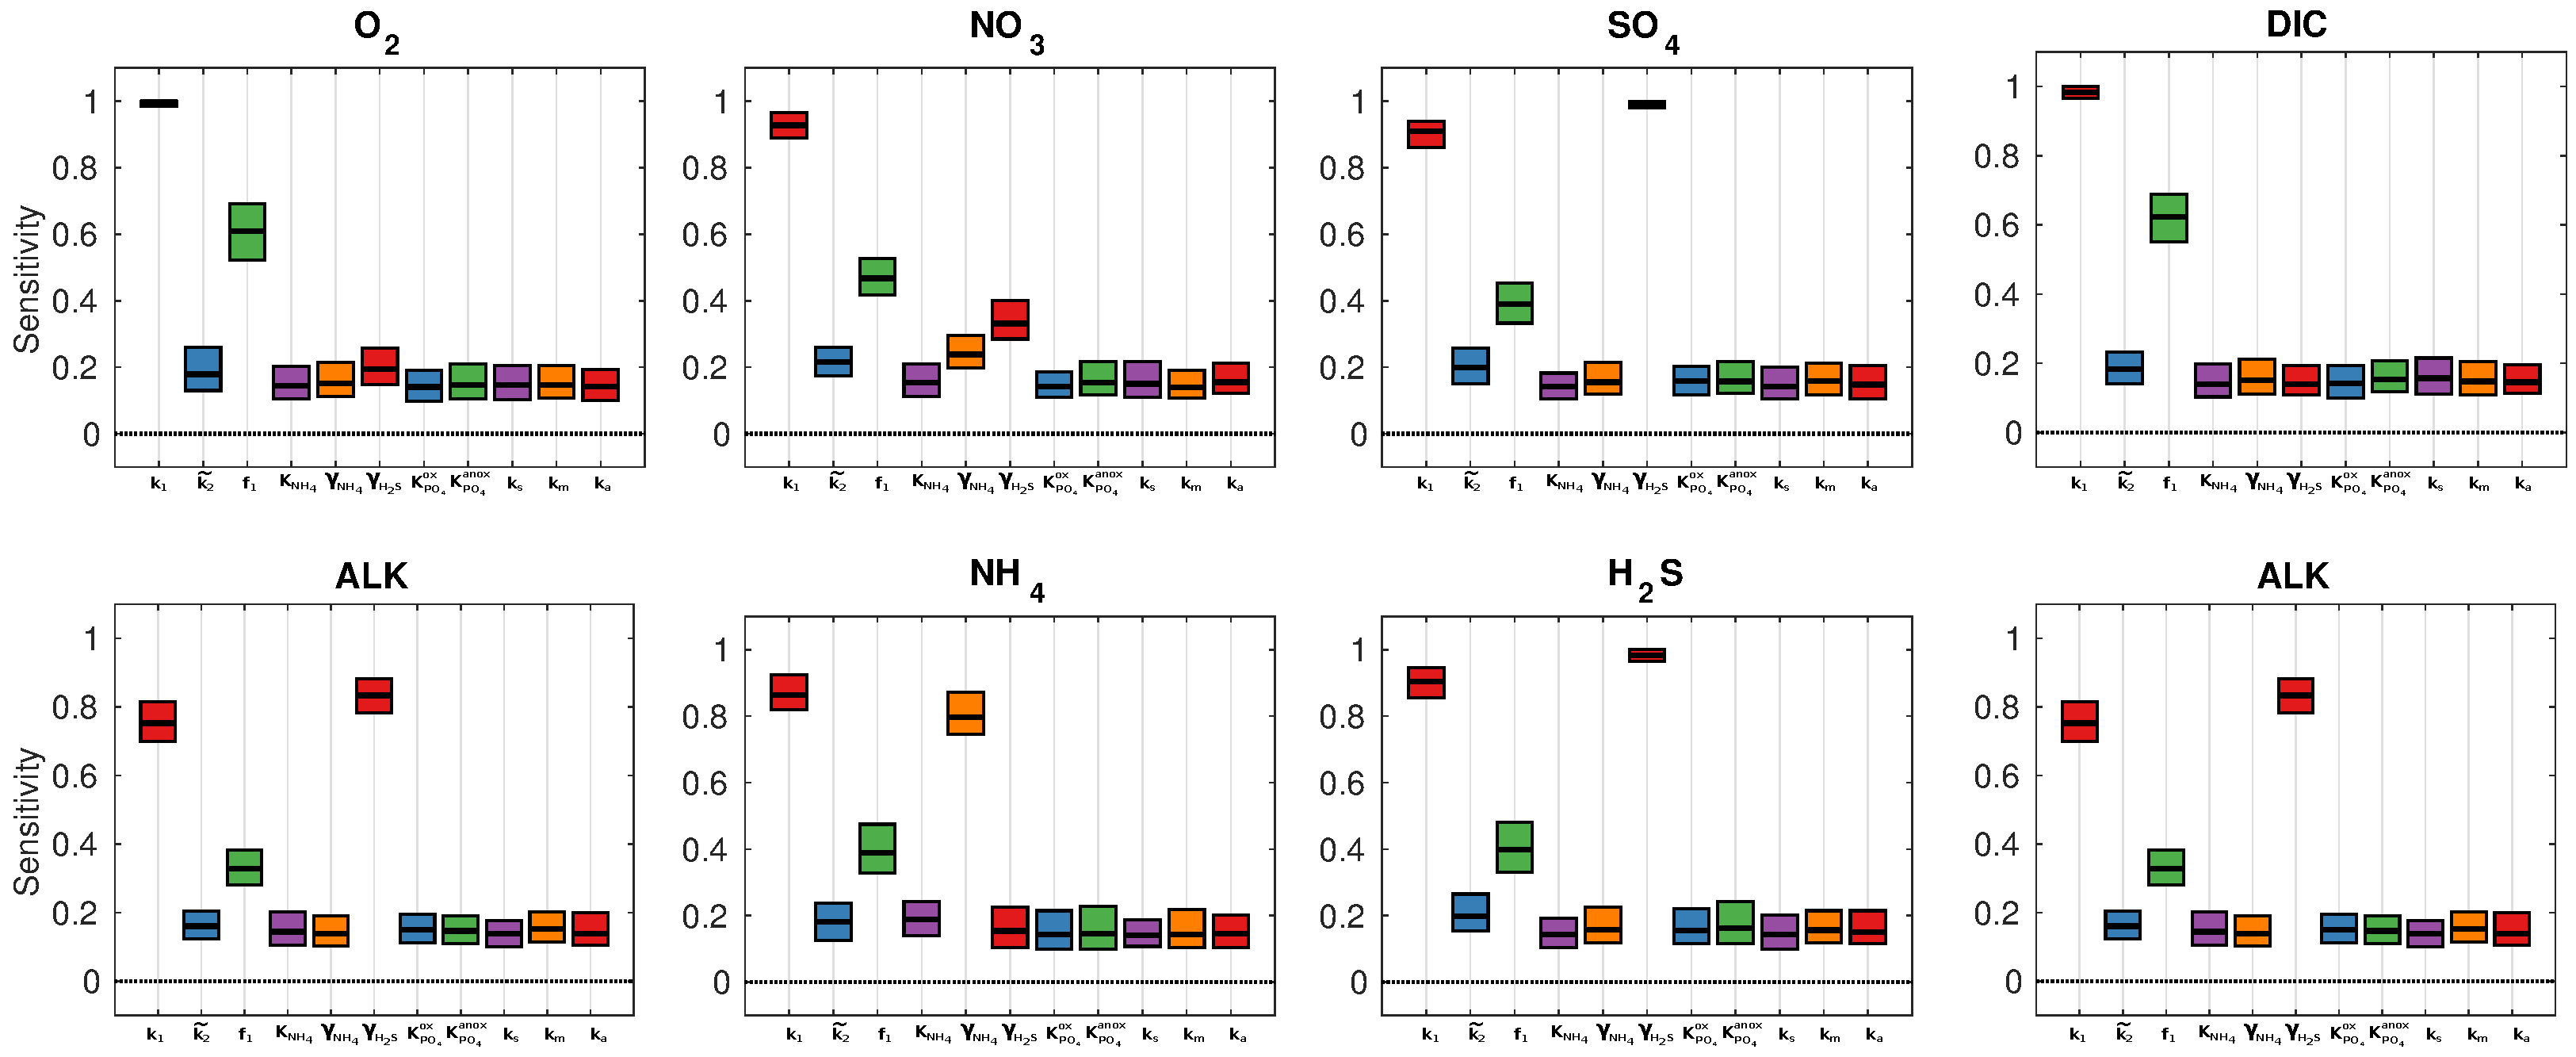
\includegraphics[width=1.0\textwidth]{figures/SA/0_SIndex_4000m_ALL_combined.pdf}
	\caption{\textcolor{red}{Move to Appendix} Box plot of parameter sensitivities for the calculated SWI-fluxes for the 4000m oxic condition. 
	Average sensitivities (black lines) and 90\% confidence intervals using $N=11200$ model evaluations and $Nboot = 100$ bootstrap resamples.}
	\label{fig:SA_O2+NO3}
	\end{center}
\end{figure}


\subsection{}                               %% Appendix A1, A2, etc.




\begin{acknowledgements}
We thank Claire Reimers and Filip Meysman for supplying the dataset from the Santa Barbara Basin, as well as Martin Thullner and Jack Middelburg for making the BRNS results and observations 
included in Section \ref{subsec:globalhypsometry} available. We are also grateful to Andy Dale for providing the global flux database used in Section \ref{subsec:SA} and 
acknowledge BODC for the OMEXDIA dataset (check CD!).
We are also grateful to Francesca Pianosi for helpful insights into sensitivity analysis. 
DH is supported by a graduate teaching studentship by the University of Bristol. SA is supported by funding from
the European Unions Horizon 2020 research and innovation programme under the Marie Sk\l{}odowska-Curie grant agreement no.
643052 (C-CASCADES). AR acknowledge funding from the EU grant ERC-2013-CoG-617313.
\end{acknowledgements}


%% REFERENCES

%% The reference list is compiled as follows:

\newpage
\bibliographystyle{apalike} %Style of Bibliography: plain / apalike / amsalpha / ...
%\bibliography{/home/alex/BRL/bib/literature/VORbib.bib} %You need a file 'literature.bib' for this.
\bibliography{Sediment_model}



%% Since the Copernicus LaTeX package includes the BibTeX style file copernicus.bst,
%% authors experienced with BibTeX only have to include the following two lines:
%%
%% \bibliographystyle{copernicus}
%% \bibliography{example.bib}
%%
%% URLs and DOIs can be entered in your BibTeX file as:
%%
%% URL = {http://www.xyz.org/~jones/idx_g.htm}
%% DOI = {10.5194/xyz}


%% LITERATURE CITATIONS
%%
%% command                        & example result
%% \citet{jones90}|               & Jones et al. (1990)
%% \citep{jones90}|               & (Jones et al., 1990)
%% \citep{jones90,jones93}|       & (Jones et al., 1990, 1993)
%% \citep[p.~32]{jones90}|        & (Jones et al., 1990, p.~32)
%% \citep[e.g.,][]{jones90}|      & (e.g., Jones et al., 1990)
%% \citep[e.g.,][p.~32]{jones90}| & (e.g., Jones et al., 1990, p.~32)
%% \citeauthor{jones90}|          & Jones et al.
%% \citeyear{jones90}|            & 1990



%% FIGURES

%% ONE-COLUMN FIGURES

%%f
%\begin{figure}[t]
%\includegraphics[width=8.3cm]{FILE NAME}
%\caption{TEXT}
%\end{figure}
%
%%% TWO-COLUMN FIGURES
%
%%f
%\begin{figure*}[t]
%\includegraphics[width=12cm]{FILE NAME}
%\caption{TEXT}
%\end{figure*}
%
%
%%% TABLES
%%%
%%% The different columns must be seperated with a & command and should
%%% end with \\ to identify the column brake.
%
%%% ONE-COLUMN TABLE
%
%%t
%\begin{table}[t]
%\caption{TEXT}
%\begin{tabular}{column = lcr}
%\tophline
%
%\middlehline
%
%\bottomhline
%\end{tabular}
%\belowtable{} % Table Footnotes
%\end{table}
%
%%% TWO-COLUMN TABLE
%
%%t
%\begin{table*}[t]
%\caption{TEXT}
%\begin{tabular}{column = lcr}
%\tophline
%
%\middlehline
%
%\bottomhline
%\end{tabular}
%\belowtable{} % Table Footnotes
%\end{table*}
%
%
%%% NUMBERING OF FIGURES AND TABLES
%%%
%%% If figures and tables must be numbered 1a, 1b, etc. the following command
%%% should be inserted before the begin{} command.
%
%\addtocounter{figure}{-1}\renewcommand{\thefigure}{\arabic{figure}a}
%
%
%%% MATHEMATICAL EXPRESSIONS
%
%%% All papers typeset by Copernicus Publications follow the math typesetting regulations
%%% given by the IUPAC Green Book (IUPAC: Quantities, Units and Symbols in Physical Chemistry,
%%% 2nd Edn., Blackwell Science, available at: http://old.iupac.org/publications/books/gbook/green_book_2ed.pdf, 1993).
%%%
%%% Physical quantities/variables are typeset in italic font (t for time, T for Temperature)
%%% Indices which are not defined are typeset in italic font (x, y, z, a, b, c)
%%% Items/objects which are defined are typeset in roman font (Car A, Car B)
%%% Descriptions/specifications which are defined by itself are typeset in roman font (abs, rel, ref, tot, net, ice)
%%% Abbreviations from 2 letters are typeset in roman font (RH, LAI)
%%% Vectors are identified in bold italic font using \vec{x}
%%% Matrices are identified in bold roman font
%%% Multiplication signs are typeset using the LaTeX commands \times (for vector products, grids, and exponential notations) or \cdot
%%% The character * should not be applied as mutliplication sign
%
%
%%% EQUATIONS
%
%%% Single-row equation
%
%\begin{equation}
%
%\end{equation}
%
%%% Multiline equation
%
%\begin{align}
%& 3 + 5 = 8\\
%& 3 + 5 = 8\\
%& 3 + 5 = 8
%\end{align}
%
%
%%% MATRICES
%
%\begin{matrix}
%x & y & z\\
%x & y & z\\
%x & y & z\\
%\end{matrix}
%
%
%%% ALGORITHM
%
%\begin{algorithm}
%\caption{�}
%\label{a1}
%\begin{algorithmic}
%�
%\end{algorithmic}
%\end{algorithm}
%
%
%%% CHEMICAL FORMULAS AND REACTIONS
%
%%% For formulas embedded in the text, please use \chem{}
%
%%% The reaction environment creates labels including the letter R, i.e. (R1), (R2), etc.
%
%\begin{reaction}
%%% \rightarrow should be used for normal (one-way) chemical reactions
%%% \rightleftharpoons should be used for equilibria
%%% \leftrightarrow should be used for resonance structures
%\end{reaction}
%
%
%%% PHYSICAL UNITS
%%%
%%% Please use \unit{} and apply the exponential notation


\end{document}